% LTeX: enabled=false
\chapter{Entre projeto e processo --- o método que
  estabelece temas, referências, técnicas e conceitos. Pensar e sentir
  através da projeção de imagens.}%
\chaptermark{Entre projeto e processo --- o método que
	estabelece temas, referências, técnicas e conceitos.}
\label{cap4-entre-projeto-processo}

Na pintura e no cinema, como vimos anteriormente, alguns dos limites
que se impõem são o quadro, o formato, a paisagem e a profundidade,
esta representada pela mesma ideia da caixa tridimensional. Tratamos
aqui de resolver o problema de como expandir a criatividade do autor,
que tem no aumento do repertório de suas referências a principal
estratégia. Assim identificamos como um aspecto importante na
construção de um projeto, antes de estabelecer técnicas para a sua
elaboração, é conhecer e experimentar algumas das múltiplas
possibilidades de criação que existem à nossa disposição. Algumas
destas técnicas são trazidas do passado, e outras têm sido incorporadas
à prática de artistas contemporâneos, como a projeção de imagens.

Neste Capítulo apresento o trabalho plástico desenvolvido no ateliê do
mestrado, com o trajeto das experimentações de processos e técnicas de
pintura a óleo, realizadas durante o período desta investigação. O
objetivo é definir processos adequados à elaboração de diferentes
projetos artísticos, temas e conceitos. Assuntos explorados nesta
dissertação, como por exemplo o do espaço profundo no cinema,
vincularam-se ao projeto expositivo pessoal intitulado \enquote{O olhar
	do cinema.}

O detalhamento das questões relativas ao movimento dos olhos, dentro do
plano cinematográfico, já tratados no
\cref{cap2-impacto-evolucao-otica}, foi o que me fez pensar em avançar
com uma proposta de projeto de pintura inspirado na estrutura visual em
questão. Ou seja, a ideia seria partir do cinema para a pintura, por
meio dos elementos considerados por Block. Em consequência, decidi
criar pinturas que evidenciassem o elemento espaço. A intenção era
observar não só os conceitos aplicados ao espaço profundo e plano, mas
também criar algumas séries que se relacionassem com imagens
recorrentes na investigação que estava realizando.

Foi necessário pensar uma metodologia para formatar o projeto plástico
pictórico que estava se sedimentando com o título \emph{Olhar do
	Cinema}. O curso \emph{Elaboração de Projetos Artísticos}, da Escola
Núcleo Academy, voltado para organizar a produção, ajudou a estruturar
este método.

Entretanto, se faz necessário apresentar outros projetos que já estavam
em desenvolvimento no período entre 2020 e 2022, como o da \emph{Mala}
e do \emph{Balanço}, e marcaram algumas bases desta investigação.
Naquele período eu criei mapas para controlar o processo de produção de
séries, durante a disciplina \emph{Estúdio de Pintura}, e construí
alguns fluxogramas:

\clearpage

\begin{quadro}
  \centering
  \caption{Mapa Processo Estúdio de Pintura 1--3}
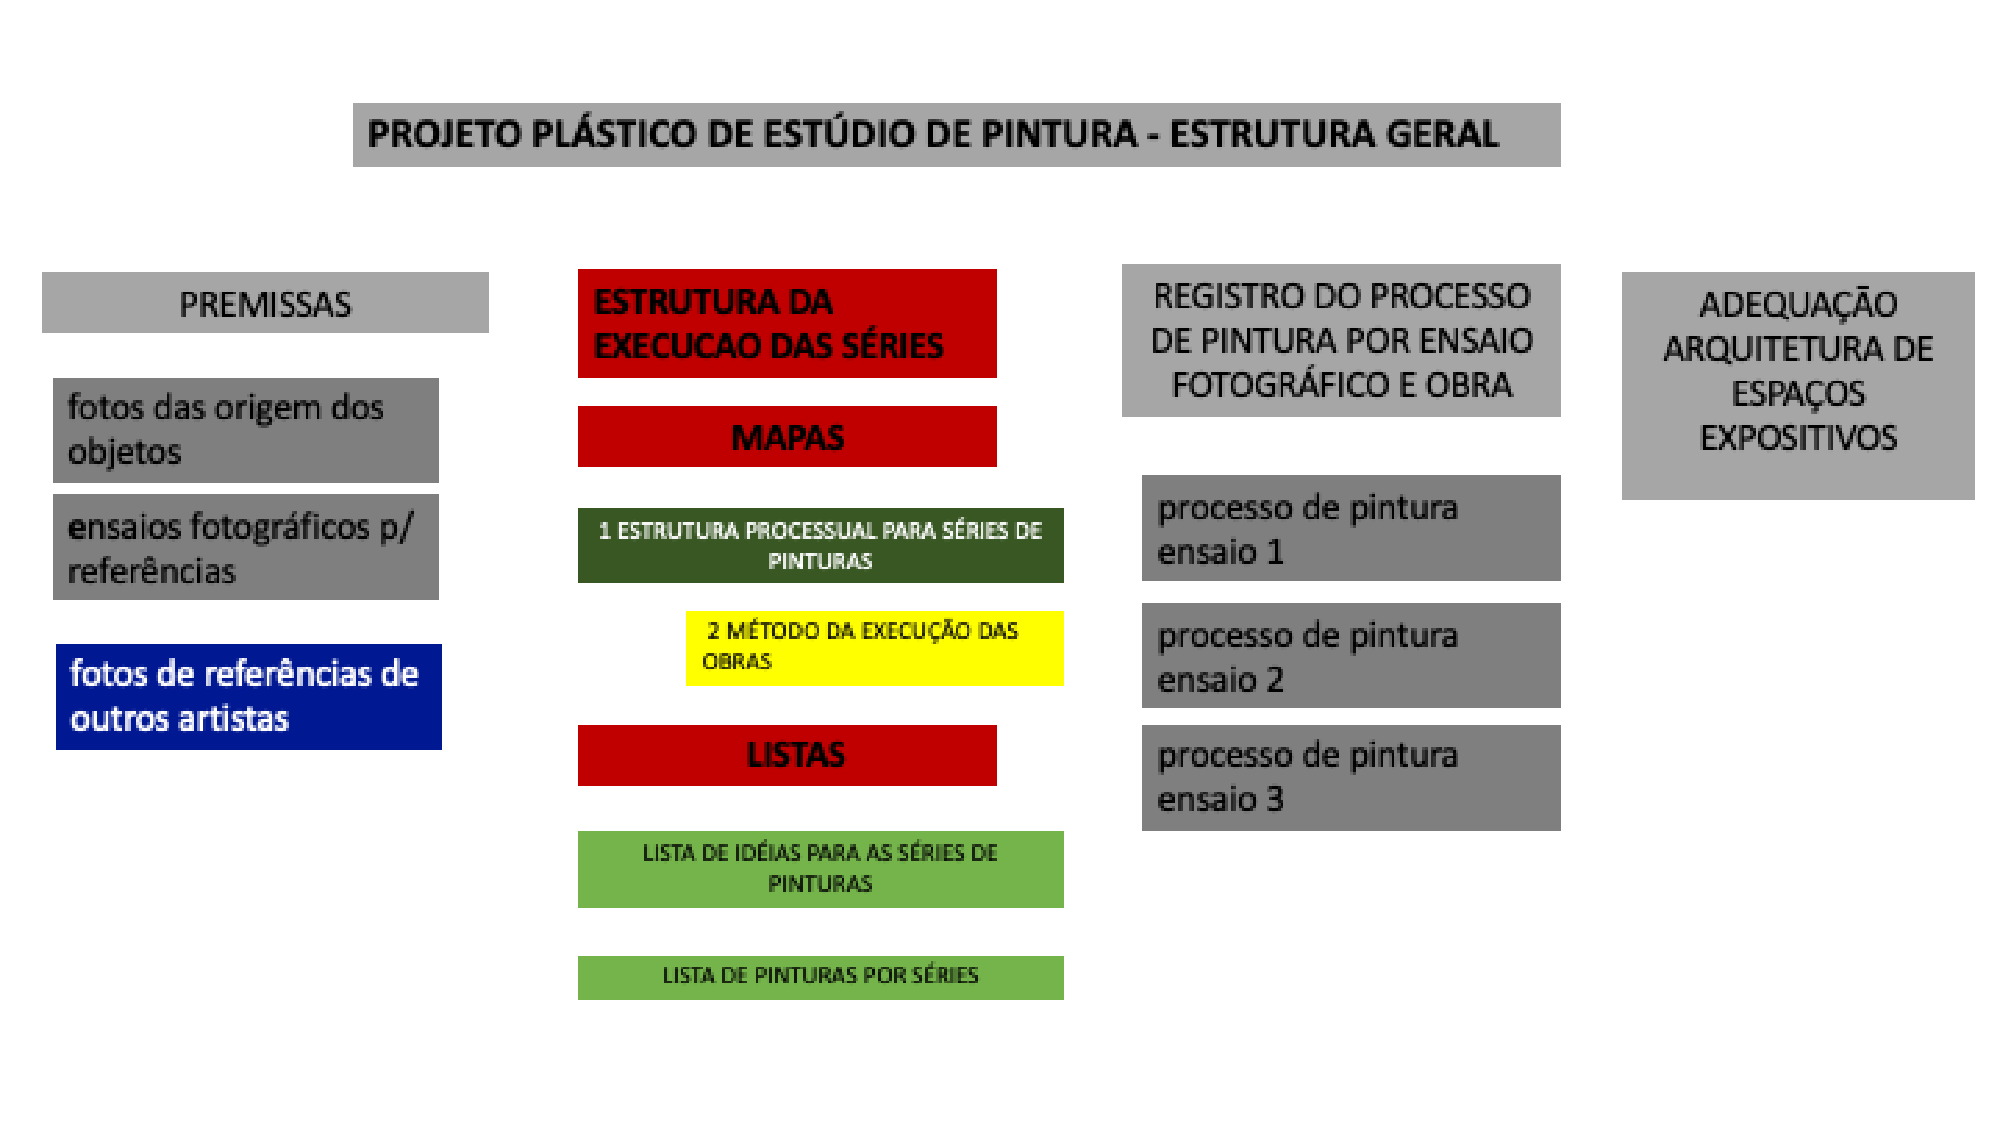
\includegraphics[width=\linewidth]{figuras/quadros/mapa-processo-estudio-pintura1.pdf}
\end{quadro}

\vfill

\begin{quadro}
  \centering
  \caption{Mapa Processo Estúdio de Pintura 2--3}
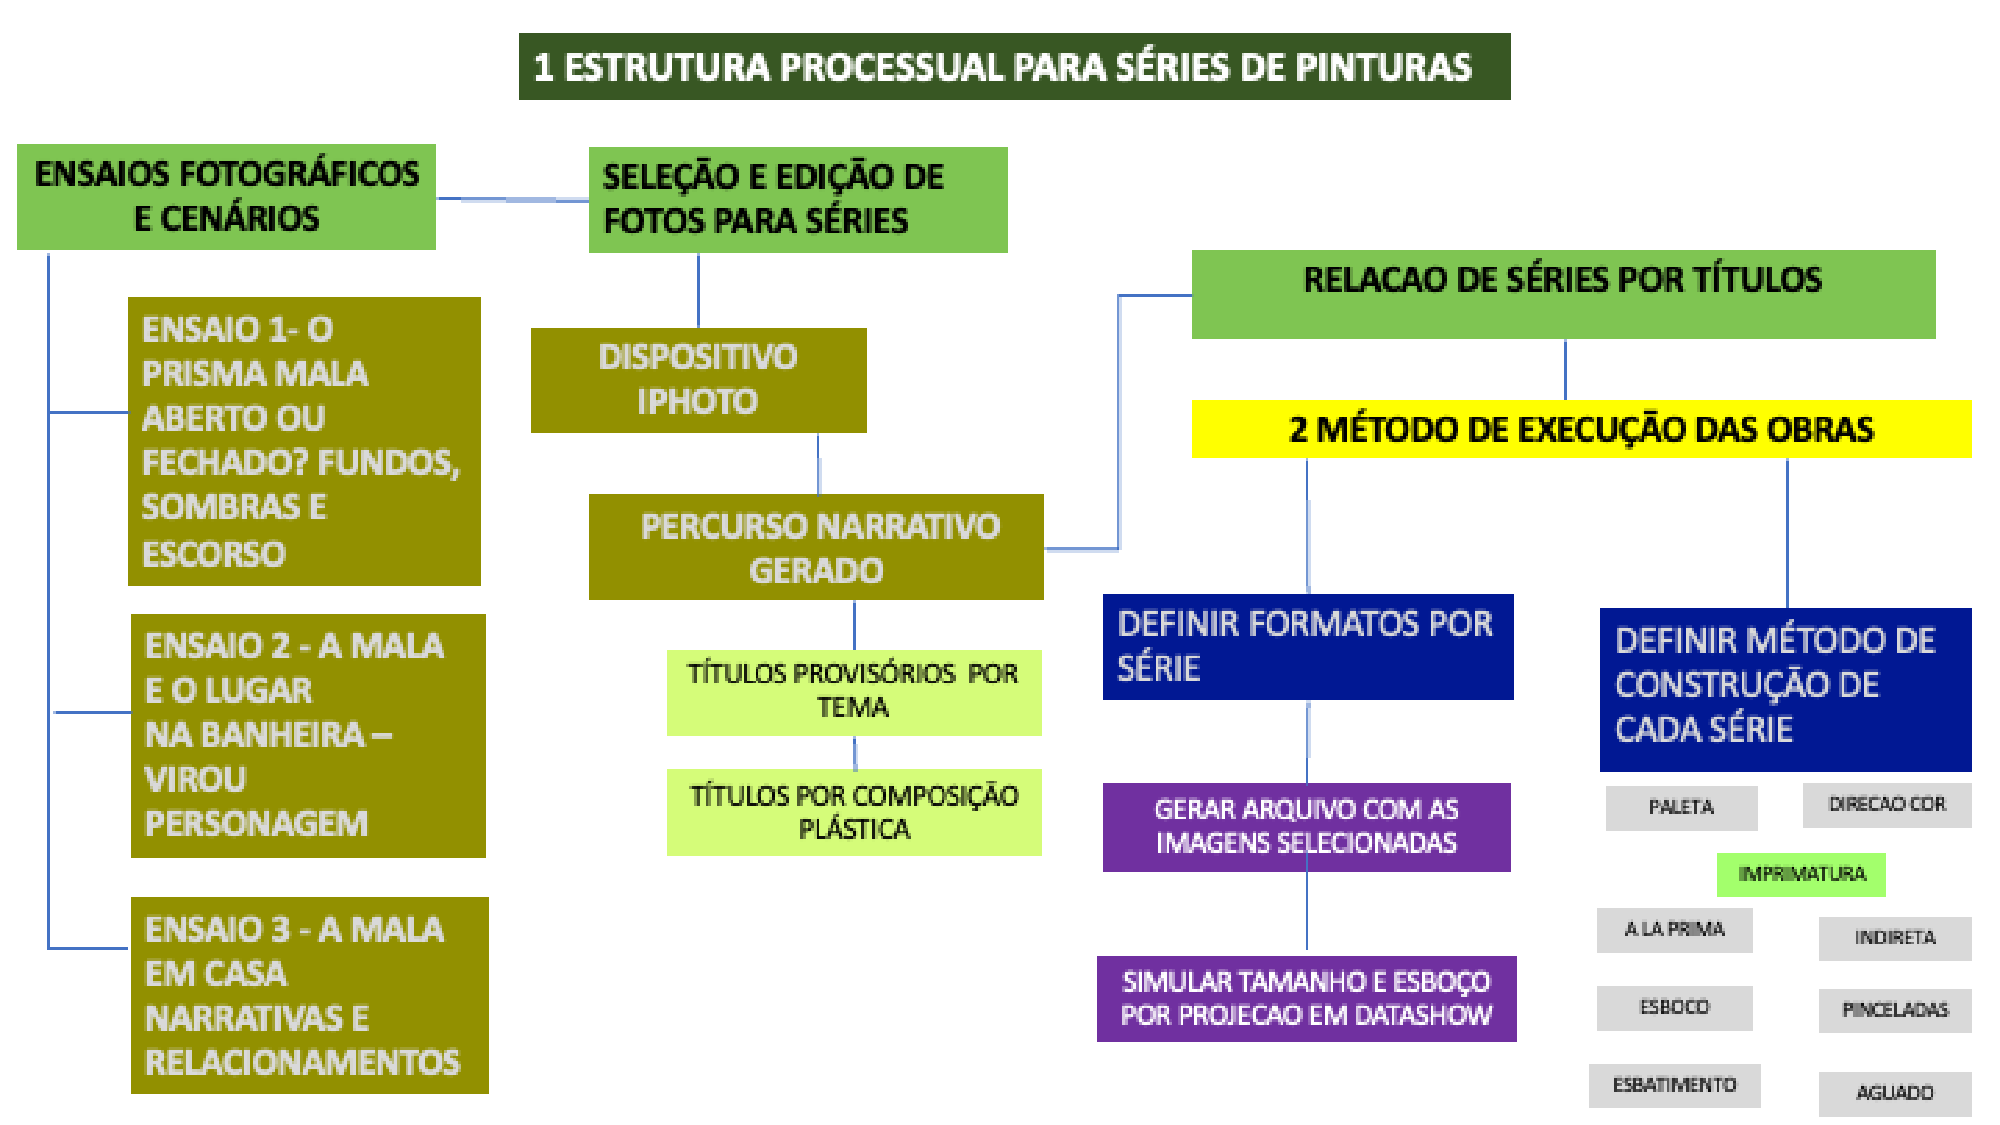
\includegraphics[width=\linewidth]{figuras/quadros/mapa-processo-estudio-pintura2.pdf}
\end{quadro}
\clearpage

\begin{quadro}
  \centering
  \caption{Mapa Processo Estúdio de Pintura 3--3}
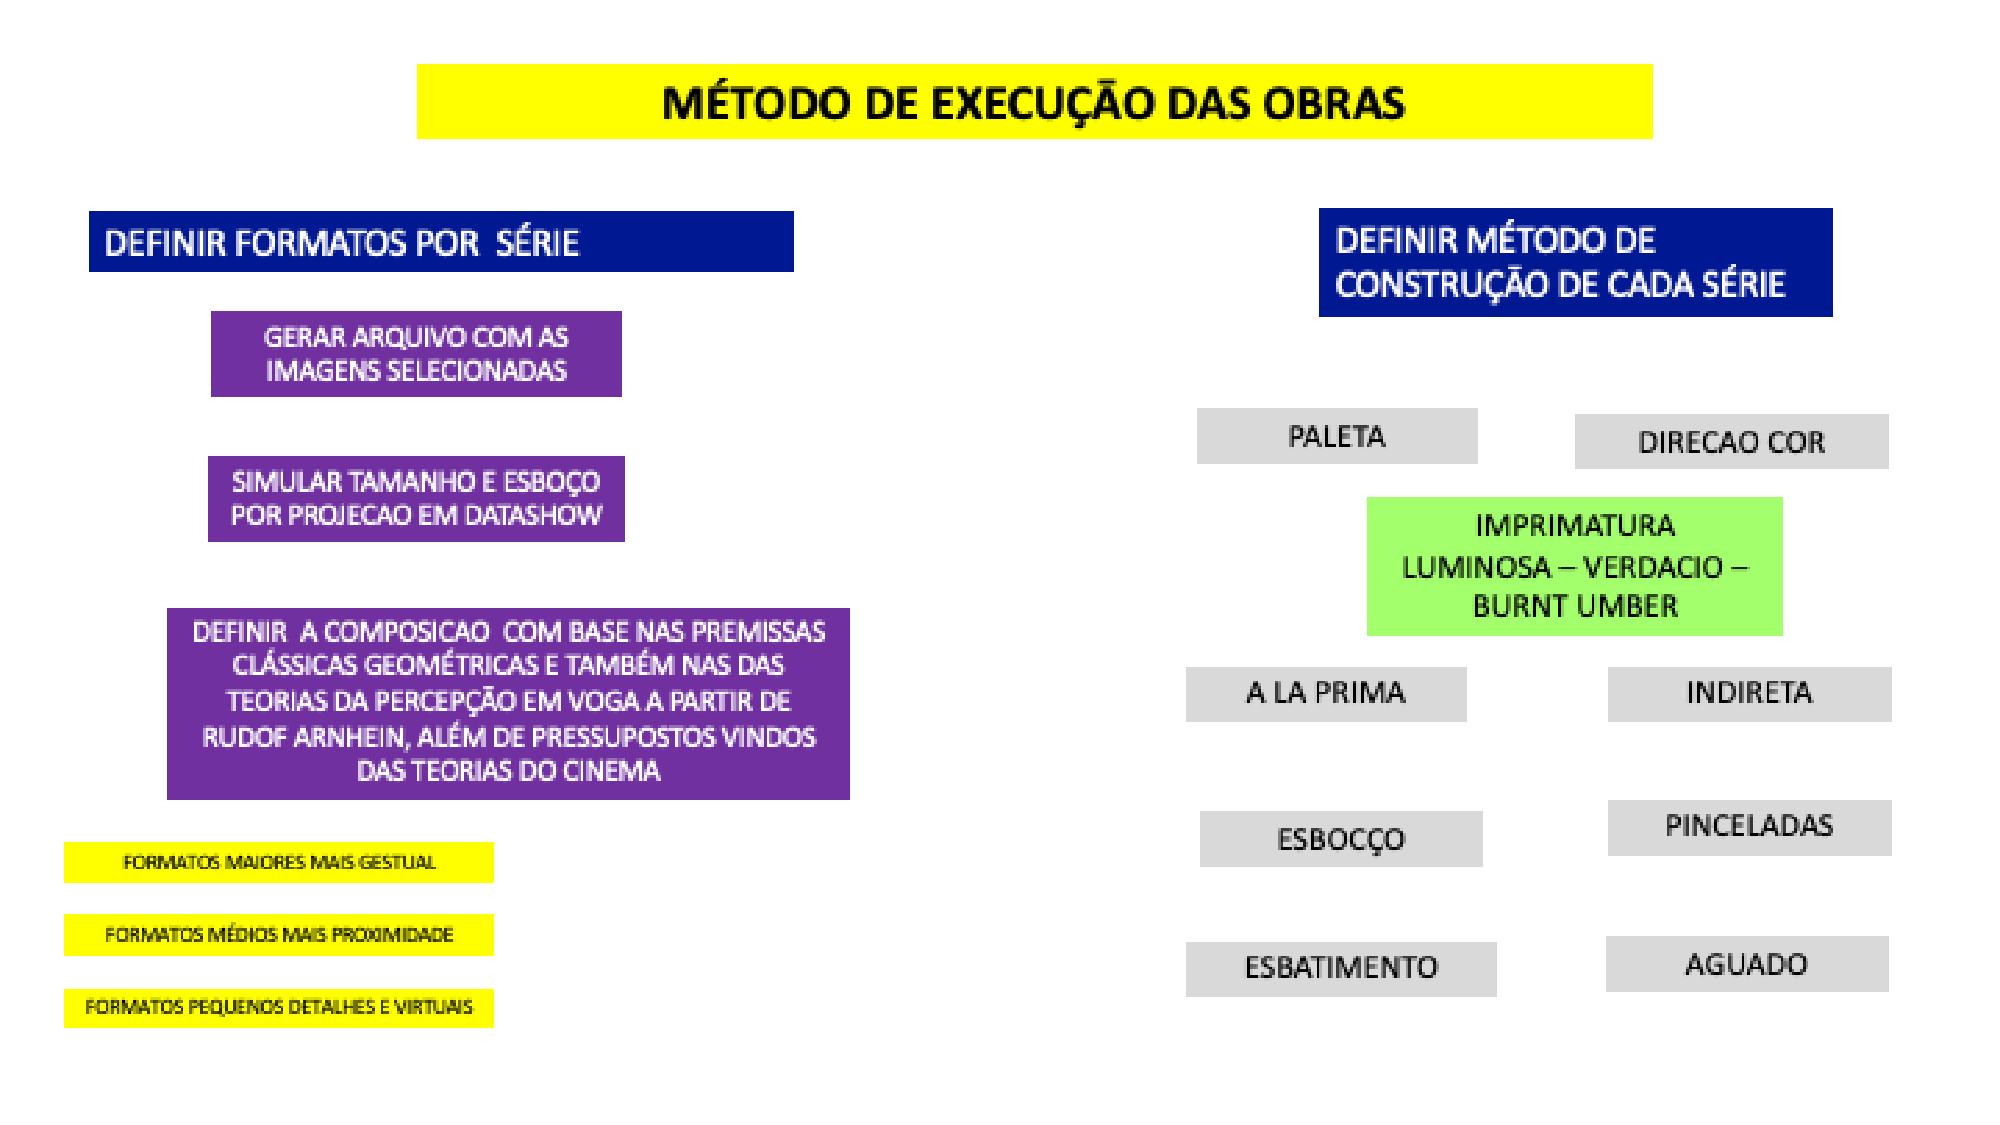
\includegraphics[width=\linewidth]{figuras/quadros/mapa-processo-estudio-pintura3.pdf}
\end{quadro}

Eu pesquisava o significado dos objetos na pintura figurativa e, em
2019, aqui em Portugal, adotei as malas como tema principal da minha
investigação. Este tema trazia consigo diversos significados
metafóricos. A intenção era colocar as malas diante de mim, talvez para
entender alguns dos sentimentos relacionados à Migração, ao Movimento
ou Deslocamento e à Perda. Uma das primeiras pinturas que realizei com
este tema foi \emph{Madra Inglesa}, da série \emph{Escorço}.

\begin{figure}
	\caption{\artname{\odette}{Madra Inglesa}{2021}}

	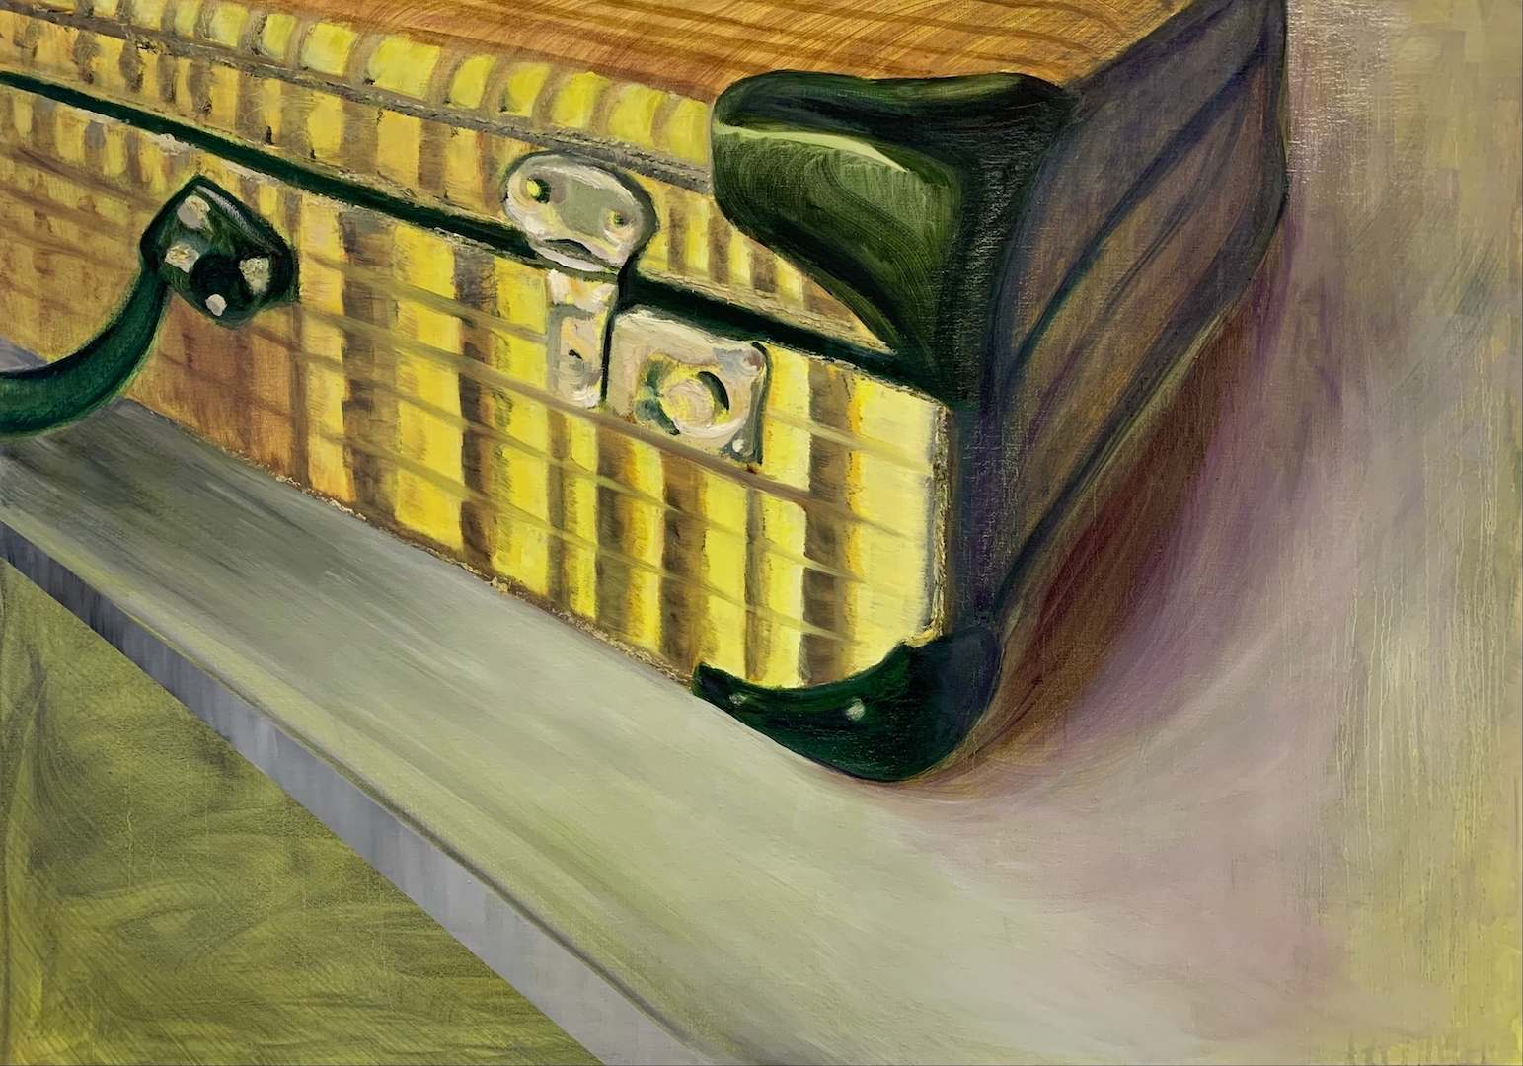
\includegraphics[width=3.87379in,height=2.71183in]{figuras/odette-madra-inglesa-2021.pdf.compressed.pdf}
	\figurenote{\series{Escorço}. \oleolinho. \artsize{74.5 x 104.5} Fonte: \archivef}
\end{figure}

Esta mala tem uma história sobre o tecido \emph{madras} e o título da
série se conecta ao enquadramento que escolhi para fotografar a mala
vintage comprada aqui no Porto, e que é meu modelo vivo até hoje. Uma
opção técnica deste trabalho é a imprimatura amarela. Sob a perspectiva
psicológica de Rudolf Arnhein, e segundo o esquema das direções
compositivas de Wassily Kandinsky, a presença de linhas diagonais na
direção esquerda-acima para direita-abaixo caracterizariam uma oposição
dramática. Assim os significados desta pintura ganhariam um enorme
leque de possibilidades.

\begin{figure}
  \flushright
  \begin{minipage}{3.92715in+1cm}
	\caption{\artname{Exposição Dialogues}{Accumulation. Searching For The Destination}{2014}}
	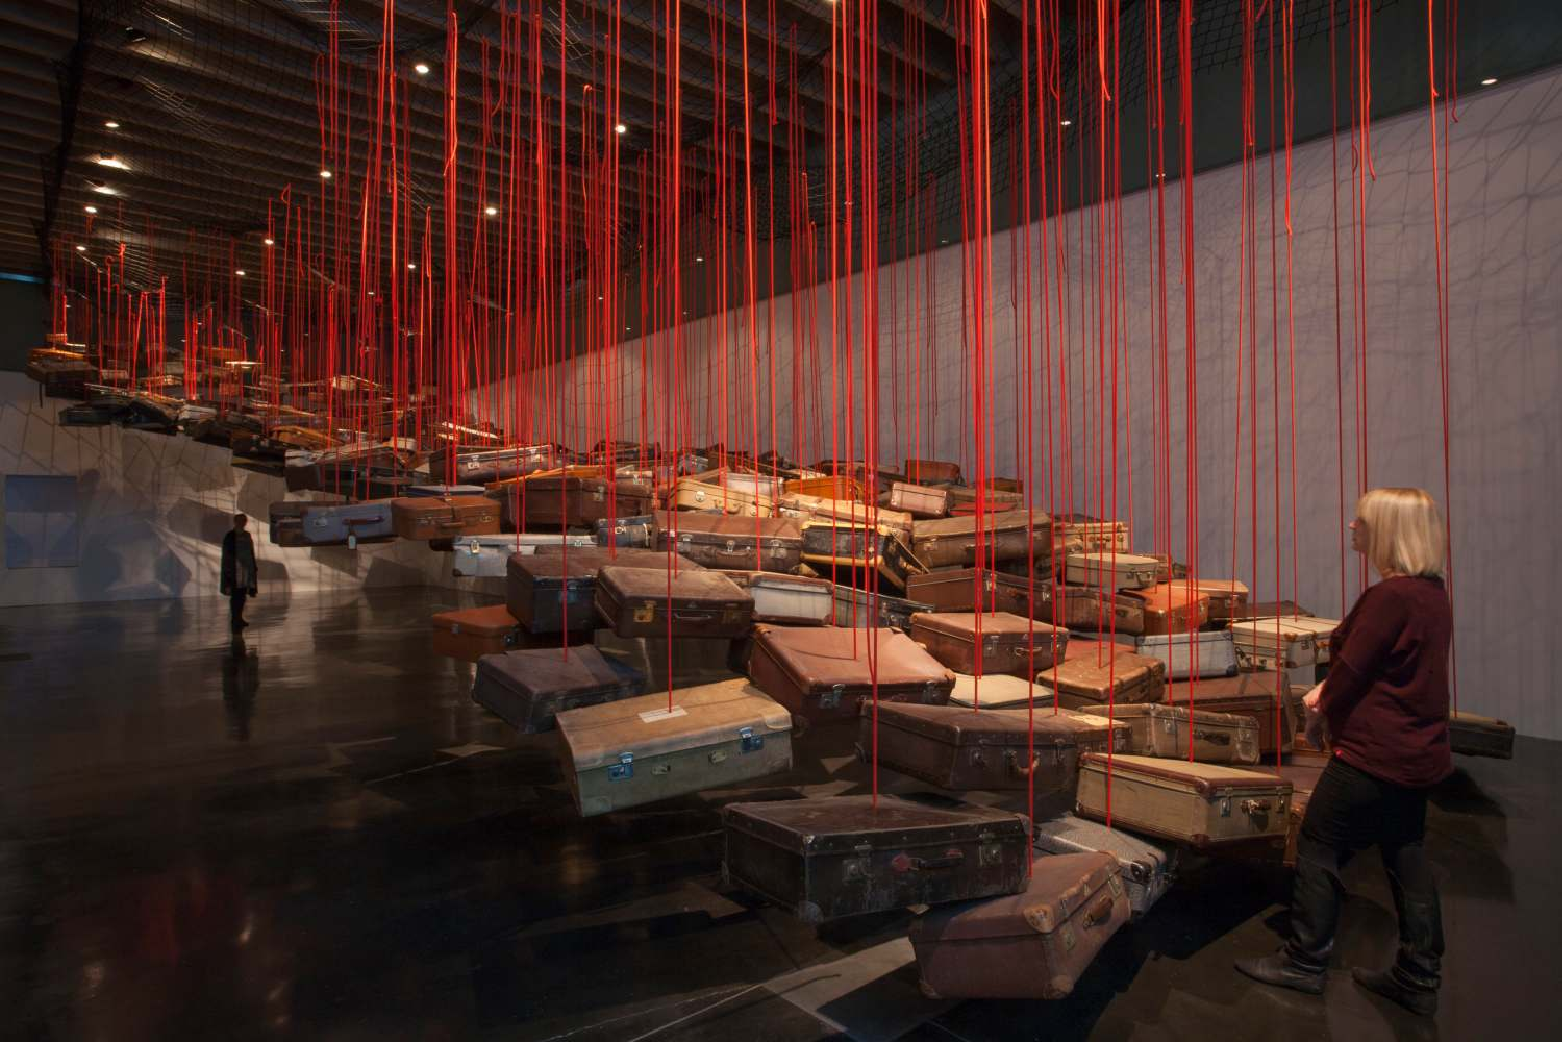
\includegraphics[width=3.52715in]{figuras/shaw-accumulation-searching-for-the-destination.pdf.compressed.pdf}
	\figurenote{Foto de Jonathan Shaw. Fonte: \hiperlink{www.chiharu-shiota.com/accumulation-searching-for-the-destination}{Website de Chiharu Shiota}}
\end{minipage}
\end{figure}


Eu buscava neste período referências na pintura e fiquei conhecendo a
artista Chiharu Shiota (1972) através da instalação \emph{Accumulation,
	Searching for a destination (2014)}.

\begin{figure}
  \begin{minipage}[t]{.45\linewidth}
	\caption{\artname{\odette}{Foto de parte do ensaio da série Penumbra}{2020}}

	\includegraphics[height=2.25in]{figuras/odette-ensaio-fotos-penumbra.pdf.compressed.pdf}
  \figurenote{Foto da autora}
\end{minipage}\hfill
\begin{minipage}[t]{.45\linewidth}
  \caption{\artname{\odette}{Chair}{2020} \phantom{aaaaaaaaaaaaaaaaaaaaaaaaaaaaaaaaaaaa}}

	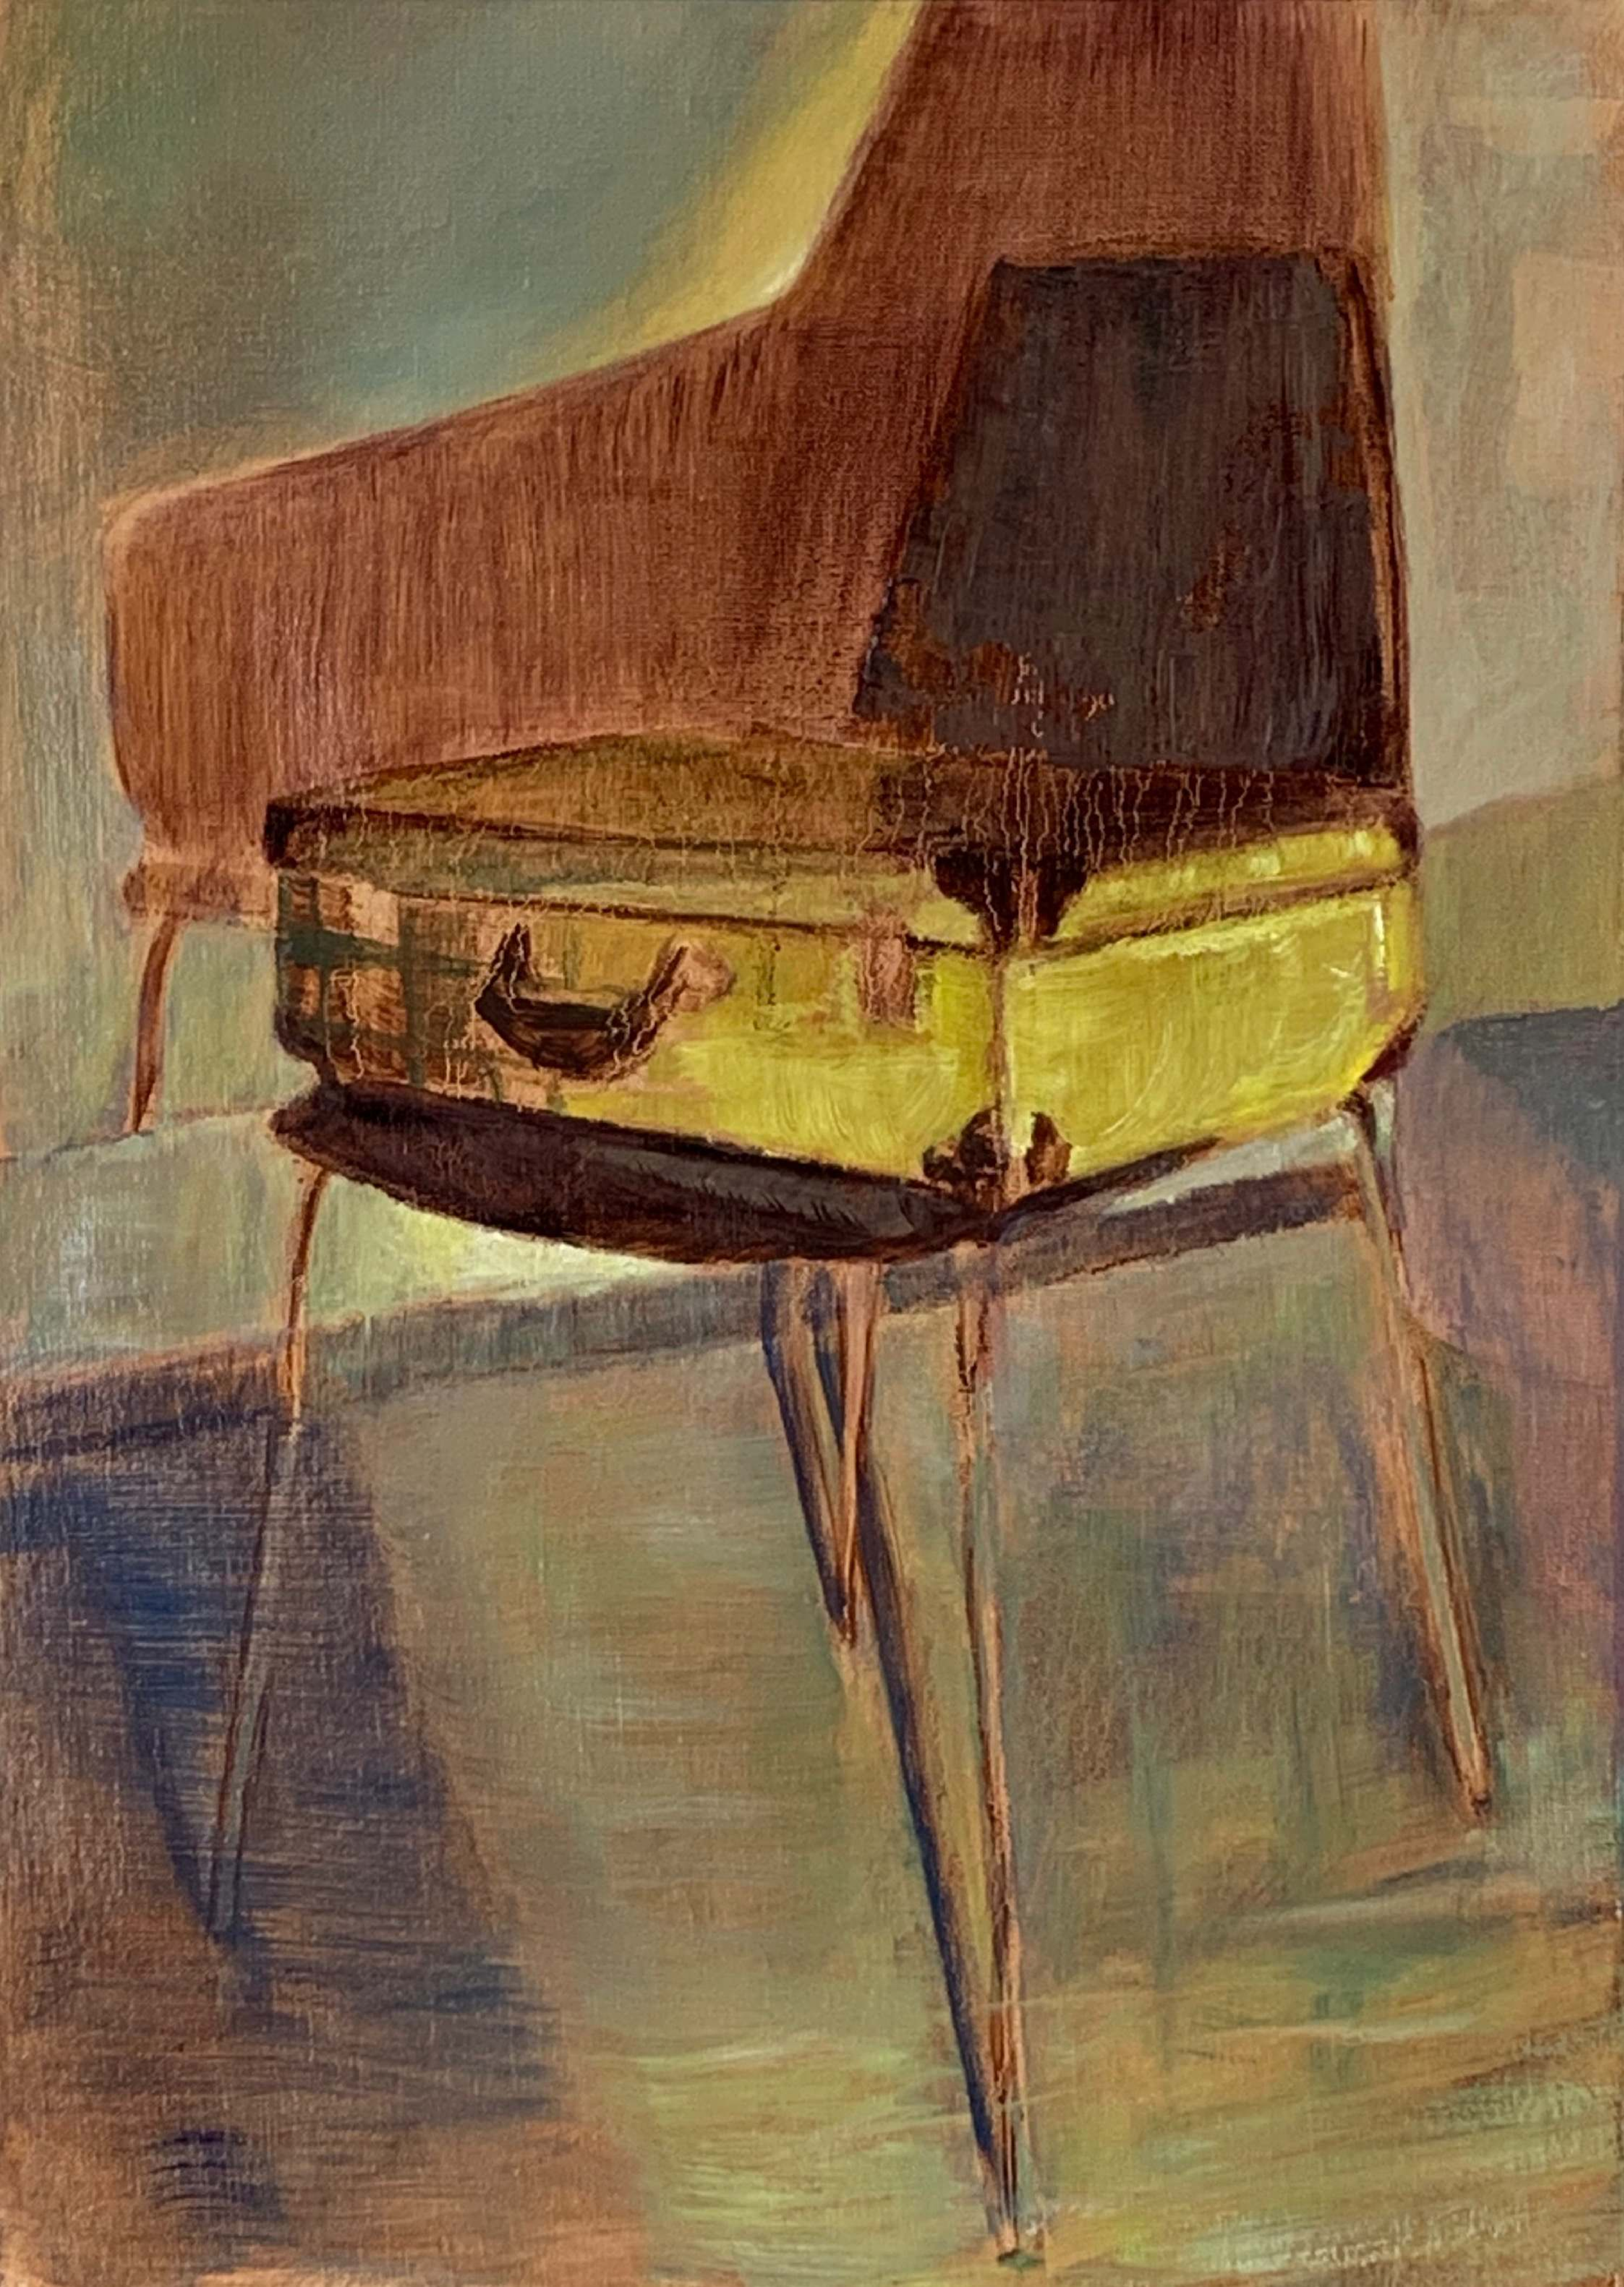
\includegraphics[height=2.25in]{figuras/odette-chair-2020.pdf.compressed.pdf}
	\figurenote{\series{Penumbra}. \oleolinho. \artsize{59.4x42x4}. \archivef}
\end{minipage}
\end{figure}
A figura da mala, e a ideia de migração, me aproximou do conceito de
movimento das imagens. A imigrante japonesa Chiharu Shiota, com a qual
meu trabalho encontrou uma grande afinidade, opera em um espaço de
transposição de meios. O cenário e os objetos das suas instalações
cinematográficas e pictóricas se aproximavam mais com o que eu queria
dizer do que as referências de pintura com o tema da mala.

O trabalho foi se desenvolvendo através de Séries como
\enquote{Penumbra} e, neste período, o meu processo se iniciava com um
ensaio de fotografias.

Depois projetava estas fotografias fazendo o esboço, num processo de
pintura indireta ou \emph{underpainting} e \emph{grisalle}, técnicas de
pintura tradicional em camadas. As malas começaram então a criar vida
própria e iniciei uma série chamada \emph{Persona}, onde este objeto se
instalava nos diversos cômodos da casa (era o período crítico da
pandemia).

Em 2021 iniciei a pintura intitulada \emph{Carregando a mala,} com
outra forma de pintar, diretamente sobre o linho branco, um processo
mais direto e rápido.

\begin{figure}
\begin{minipage}{.45\linewidth}
	\caption{\artname{\odette}{Carregando a mala}{2021}}
	\includegraphics[height=2.49903in]{figuras/odette-carregando-mala-2021-esboco.pdf}
	\figurenote{\series{Me leva}. \oleolinho. \artsize{80x80}. Fonte: \archivef}
\end{minipage}\hfill
  \begin{minipage}{.45\linewidth}
	\caption{\artname{\odette}{Carregando a mala}{2021}}
	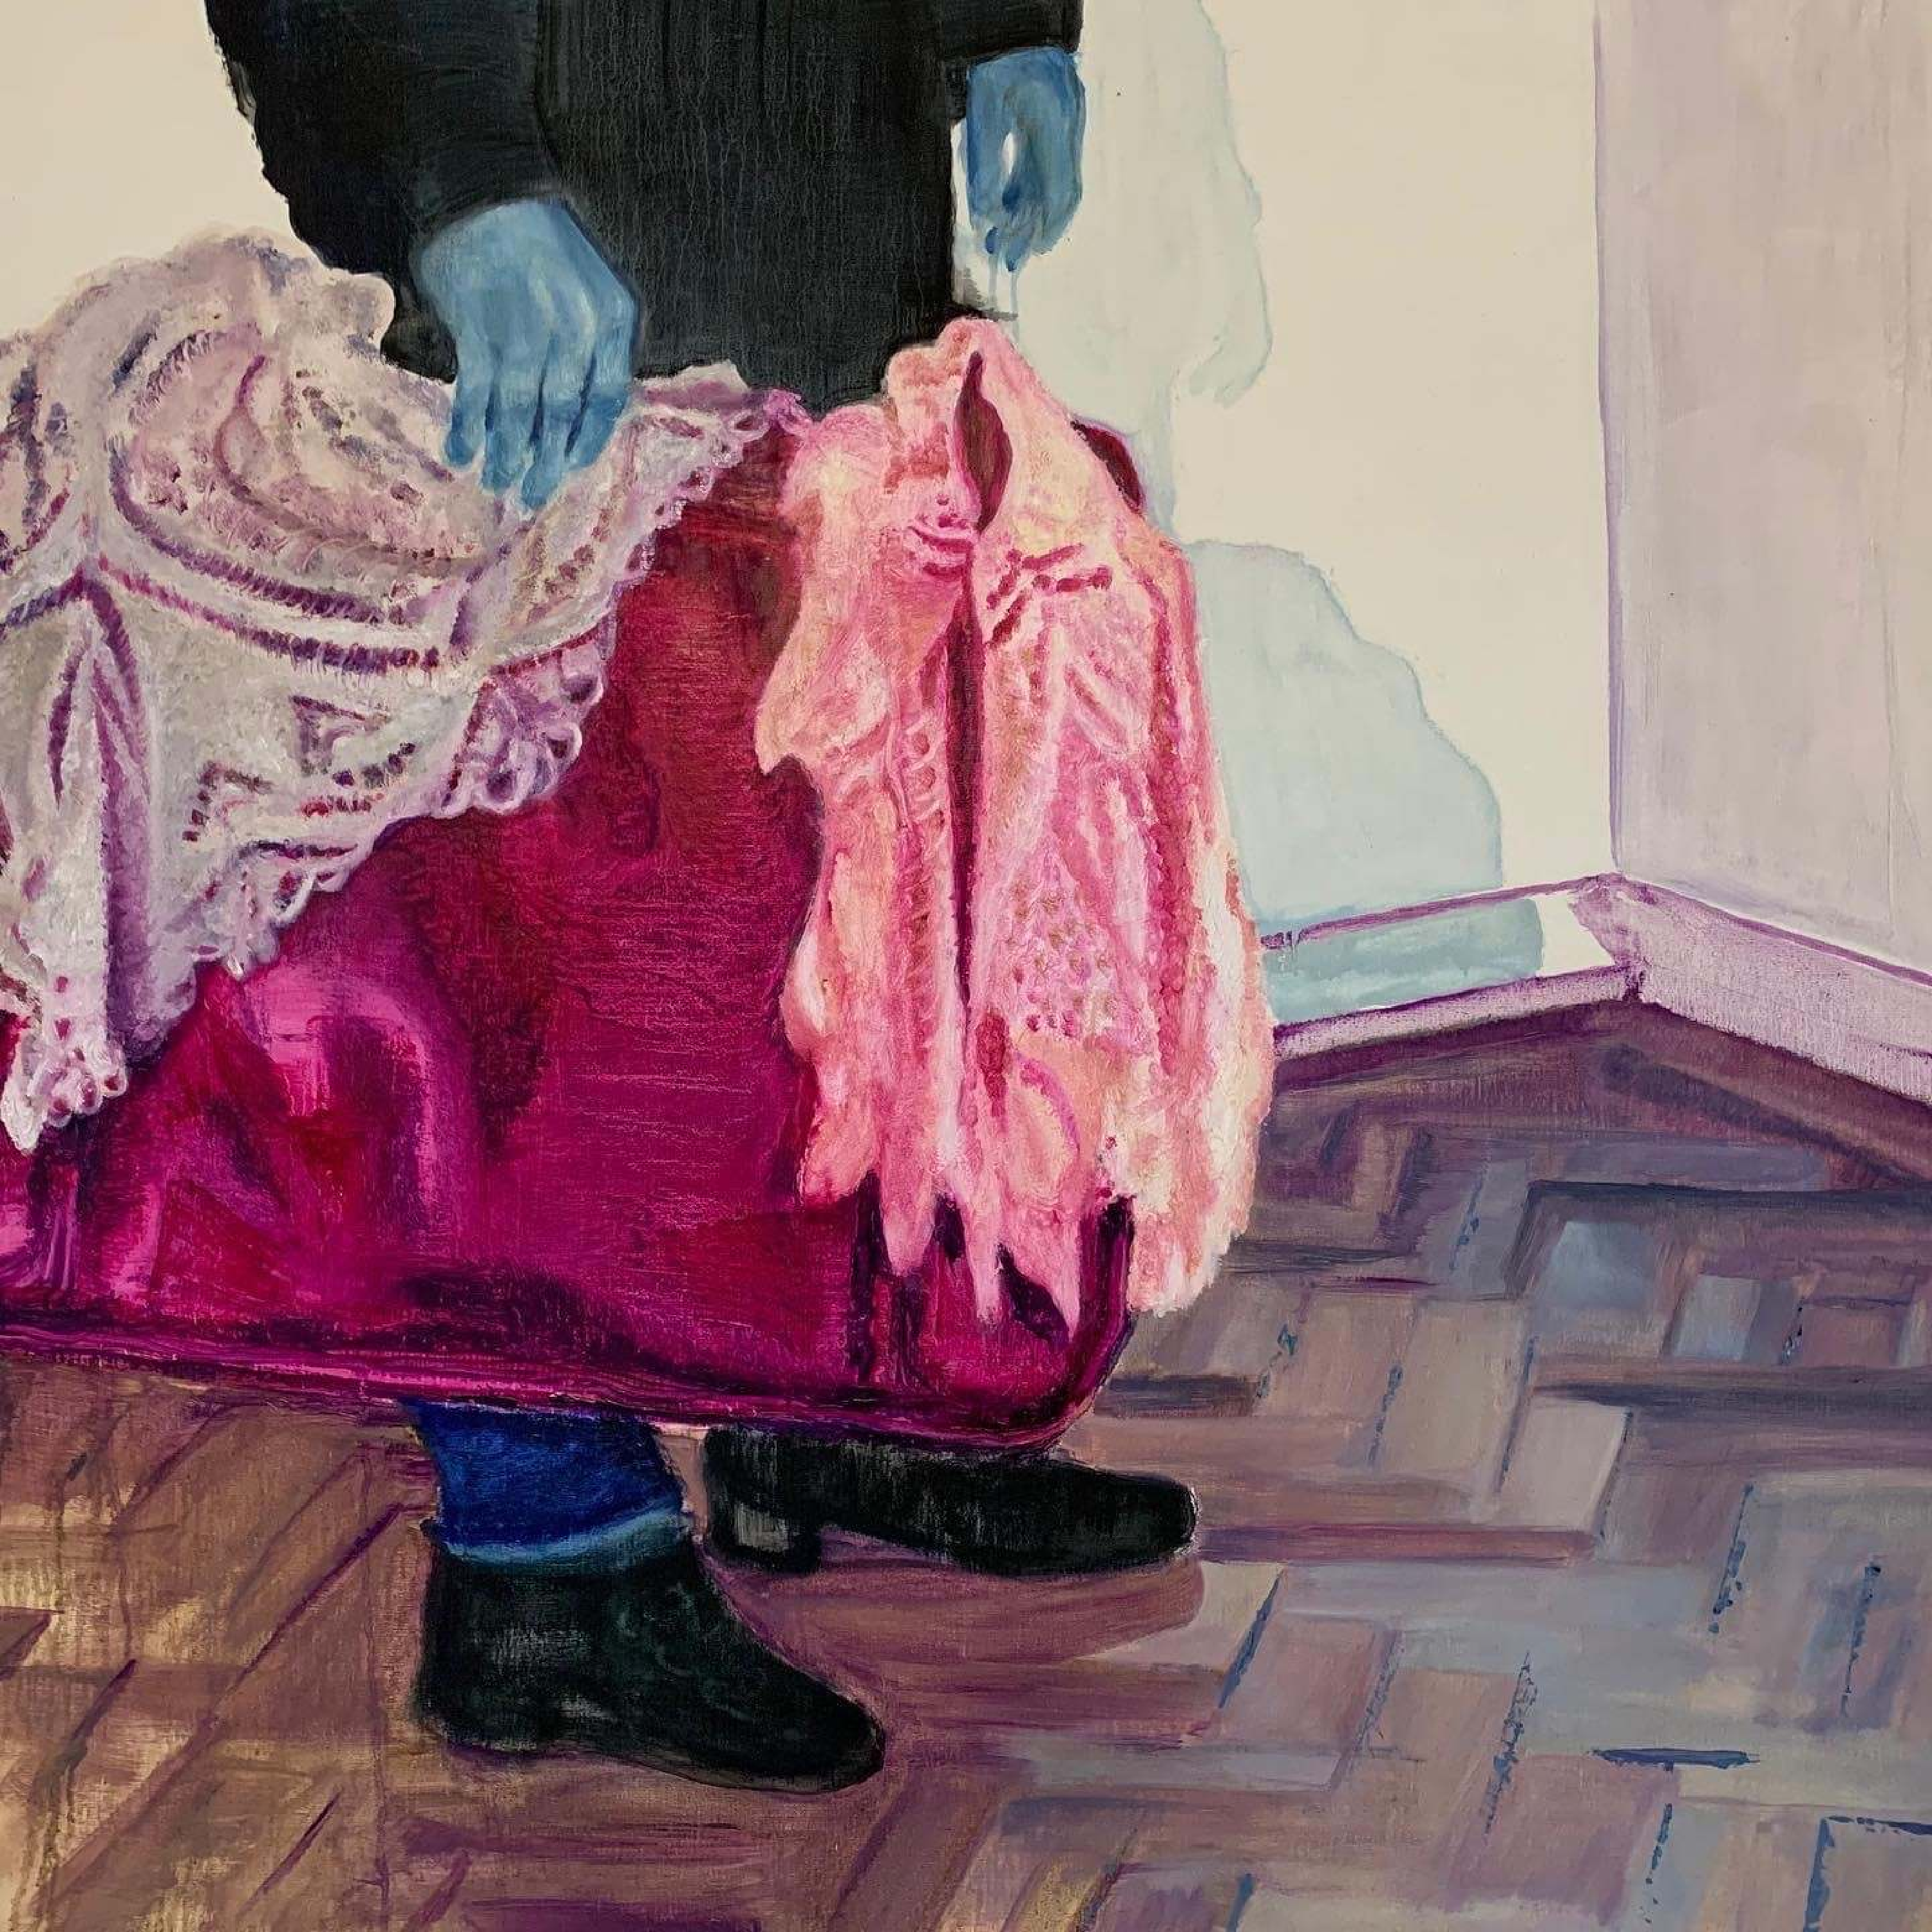
\includegraphics[height=2.49903in]{figuras/odette-carregando-mala-2021.pdf.compressed.pdf}
	\figurenote{\series{Me leva}. \oleolinho. \artsize{80x80}. Fonte: \archivef}
\end{minipage}
\end{figure}

A pintura se tornou mais fluida, mas mantendo sempre o interesse em
usar um impaste na finalização. No final de 2021, em viagem pelo
Brasil, me aventurei na linguagem tridimensional. Construí o meu
primeiro objeto instalativo, que se chama \emph{Por dois fios,} numa
alusão aos fios que nos ligam à terra. Construído com aramado de metal
e sobreposição de rendas têxteis, foi fotografado com uma iluminação de
estúdio e exposto virtualmente através do Instagram. Esta foi a última
mala que eu efetivamente criei.

\begin{figure}
  \flushright
  \begin{minipage}{3.28742in}
	\caption{\artname{\odette}{Por dois fios}{2021}}

  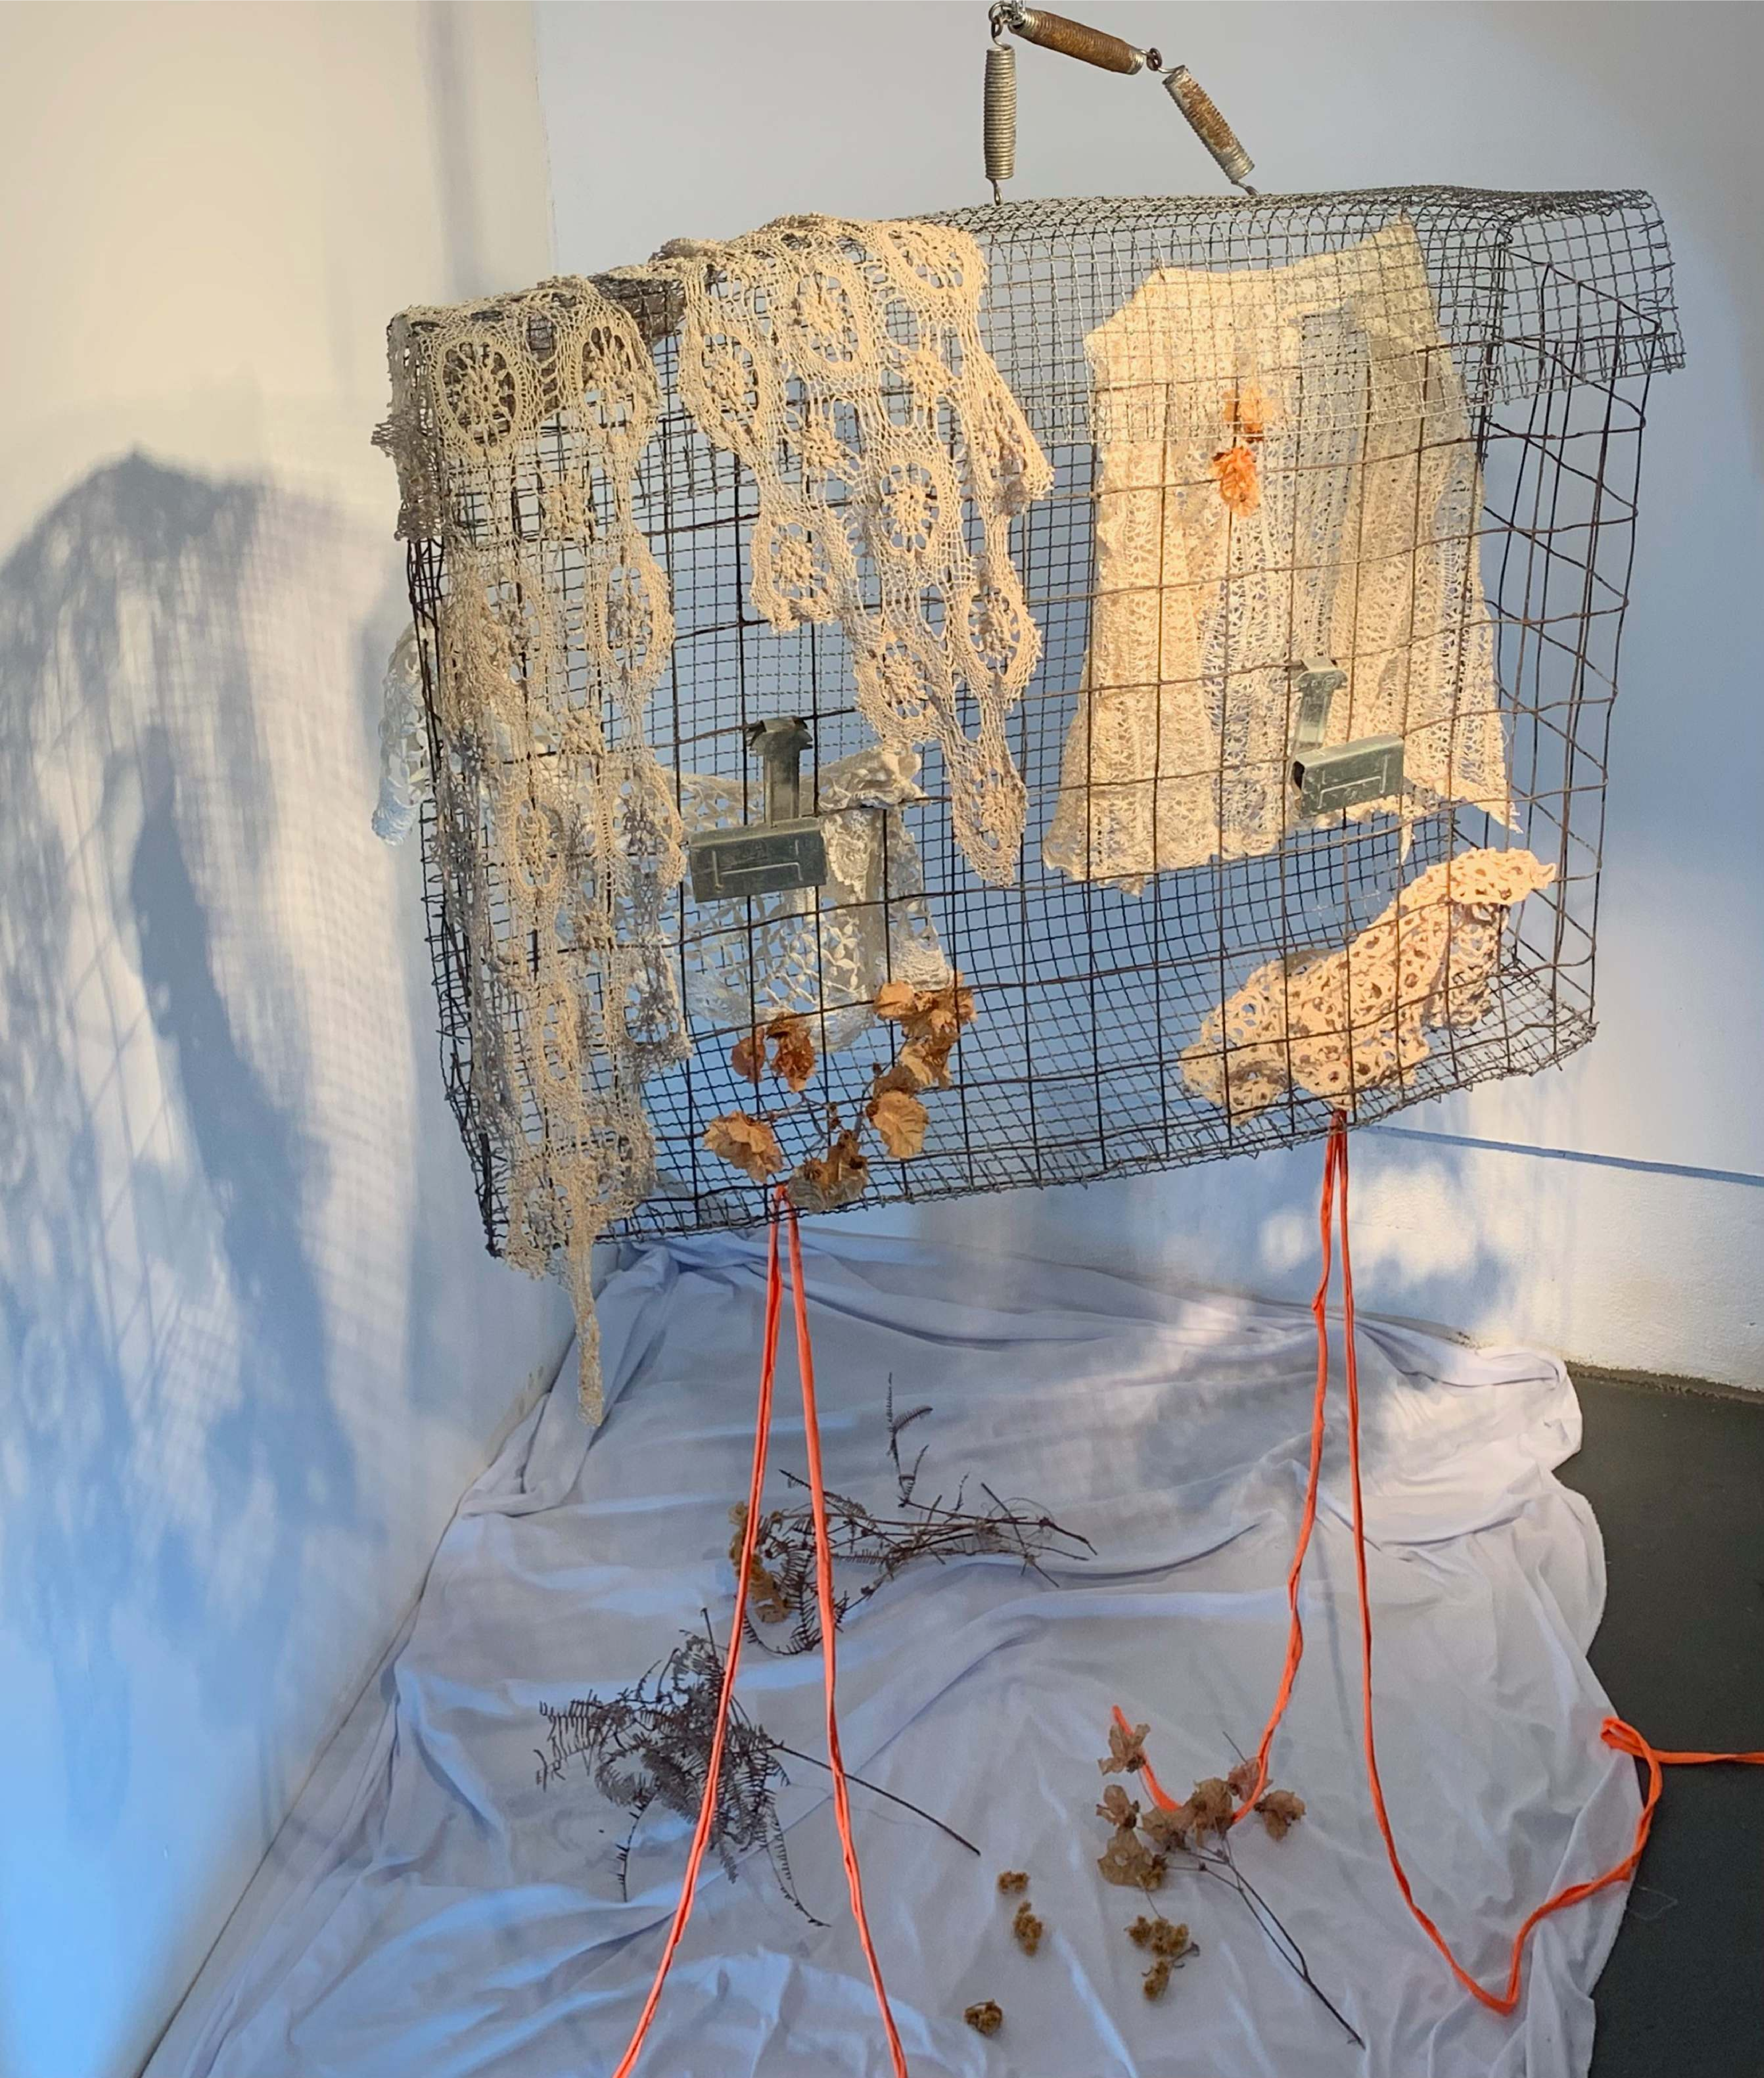
\includegraphics[width=2.7in]{figuras/odette-por-dois-fios-2021.pdf.compressed.pdf}
	\figurenote{\series{Me rendo}. Objeto instalativo. Dimensões variadas.
		Foto Adilson D'~Avilla. Fonte: \archivef}
\end{minipage}
\end{figure}

O Projeto \emph{Nem tudo é cor de Rosa} apresentou pinturas das malas
na exposição virtual \emph{paralela EIXO 2021.} A ideia era falar sobre
o cenário fantástico e inexplicável dos tempos de pandemia. Uma ideia
meio de sonho ou pesadelo. Em seguida, interessada em trabalhar em
pinturas que retratam uma atmosfera fantasiosa, iniciei uma série com
fundo verde em \emph{chroma} luminoso (na paleta \emph{viridian} e
\emph{phtalo green}). Escolhi a pintura \emph{O Balanço} (1767--1768),
de \emph{Fragonard} (1732--1806), ícone do movimento Rococó que se
iniciou no século~XVII\@. Este movimento se caracterizava por um
acúmulo de detalhes, e de muita frivolidade. Liberdade para sonhar. O
Rococó me fez pensar nos detalhes das rendas de minha coleção de
apliques usados nas costuras da minha mãe. O vestido esvoaçante e
detalhado da mocinha retomava o tema de tecidos que já havia explorado
alguns anos antes.

\begin{figure}[b]
	\caption{Estudo de elementos em colagem digital.}

	\includegraphics[width=2.79257in,height=2.09459in]{figuras/estudo-elementos-colagem-digital.pdf.compressed.pdf}
	\figurenote{Fonte: \archivef}
\end{figure}

Partindo da técnica de colagem, não a tradicional, mas digital,
realizei uma espécie de decupagem,\footnote{Decupagem in Priberam ---
	2.~\textins{Cinema, Televisão}~Divisão de um texto em cenas e planos,
	com escolhas e anotações técnicas e cênicas~para gravação ou filmagem.}
pintei um céu com um balanço em 3 posições, simulando o movimento de um
pêndulo. Embora já trabalhasse com pintura há muitos anos, esta foi a
primeira vez que experimentei a colagem, para pensar a composição de
elementos e narrativa dentro de um cenário.

\begin{figure}
  \begin{minipage}{.45\linewidth}
	\caption{Estudo com base em decupagem de elementos da colagem}

	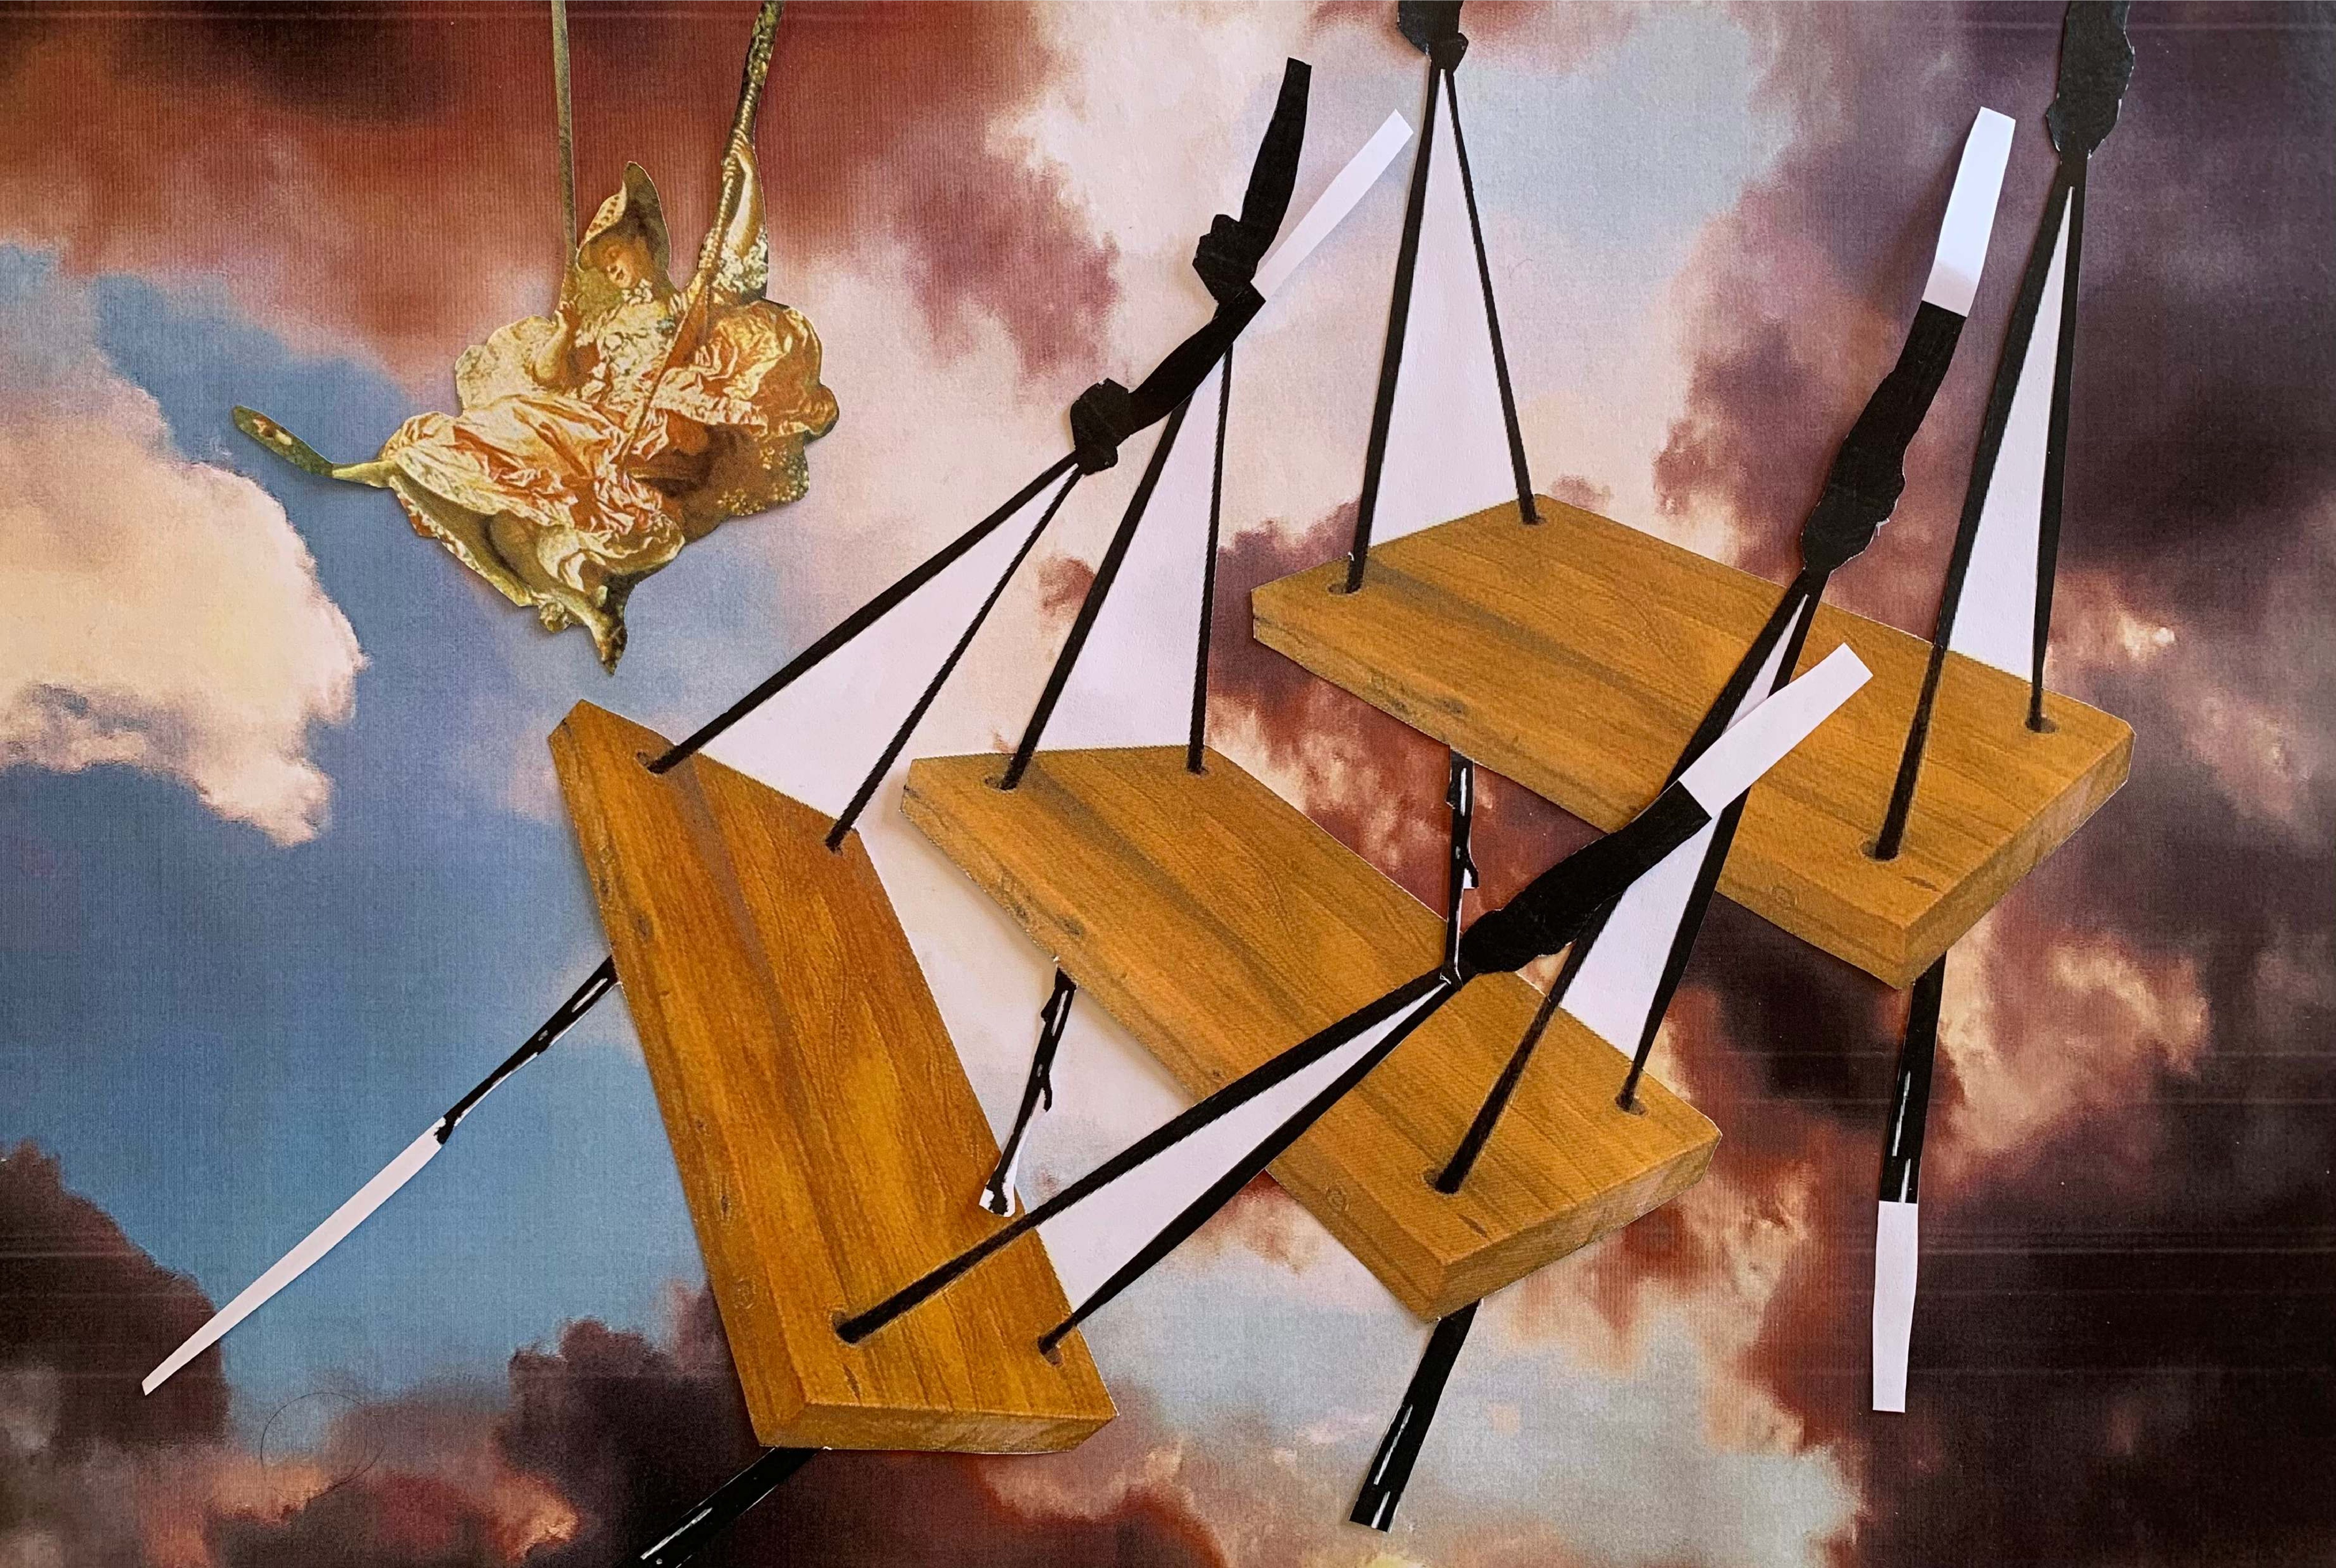
\includegraphics[width=2.84478in,height=1.89189in]{figuras/estudo-decupagem-elementos-colagem.pdf.compressed.pdf}
	\figurenote{Fonte: \archivef}
\end{minipage}\hfill
\begin{minipage}{.45\linewidth}
  \caption{Estudo para projeção por exclusão de matizes \phantom{aaaaaaaaaaaaaaa}}
	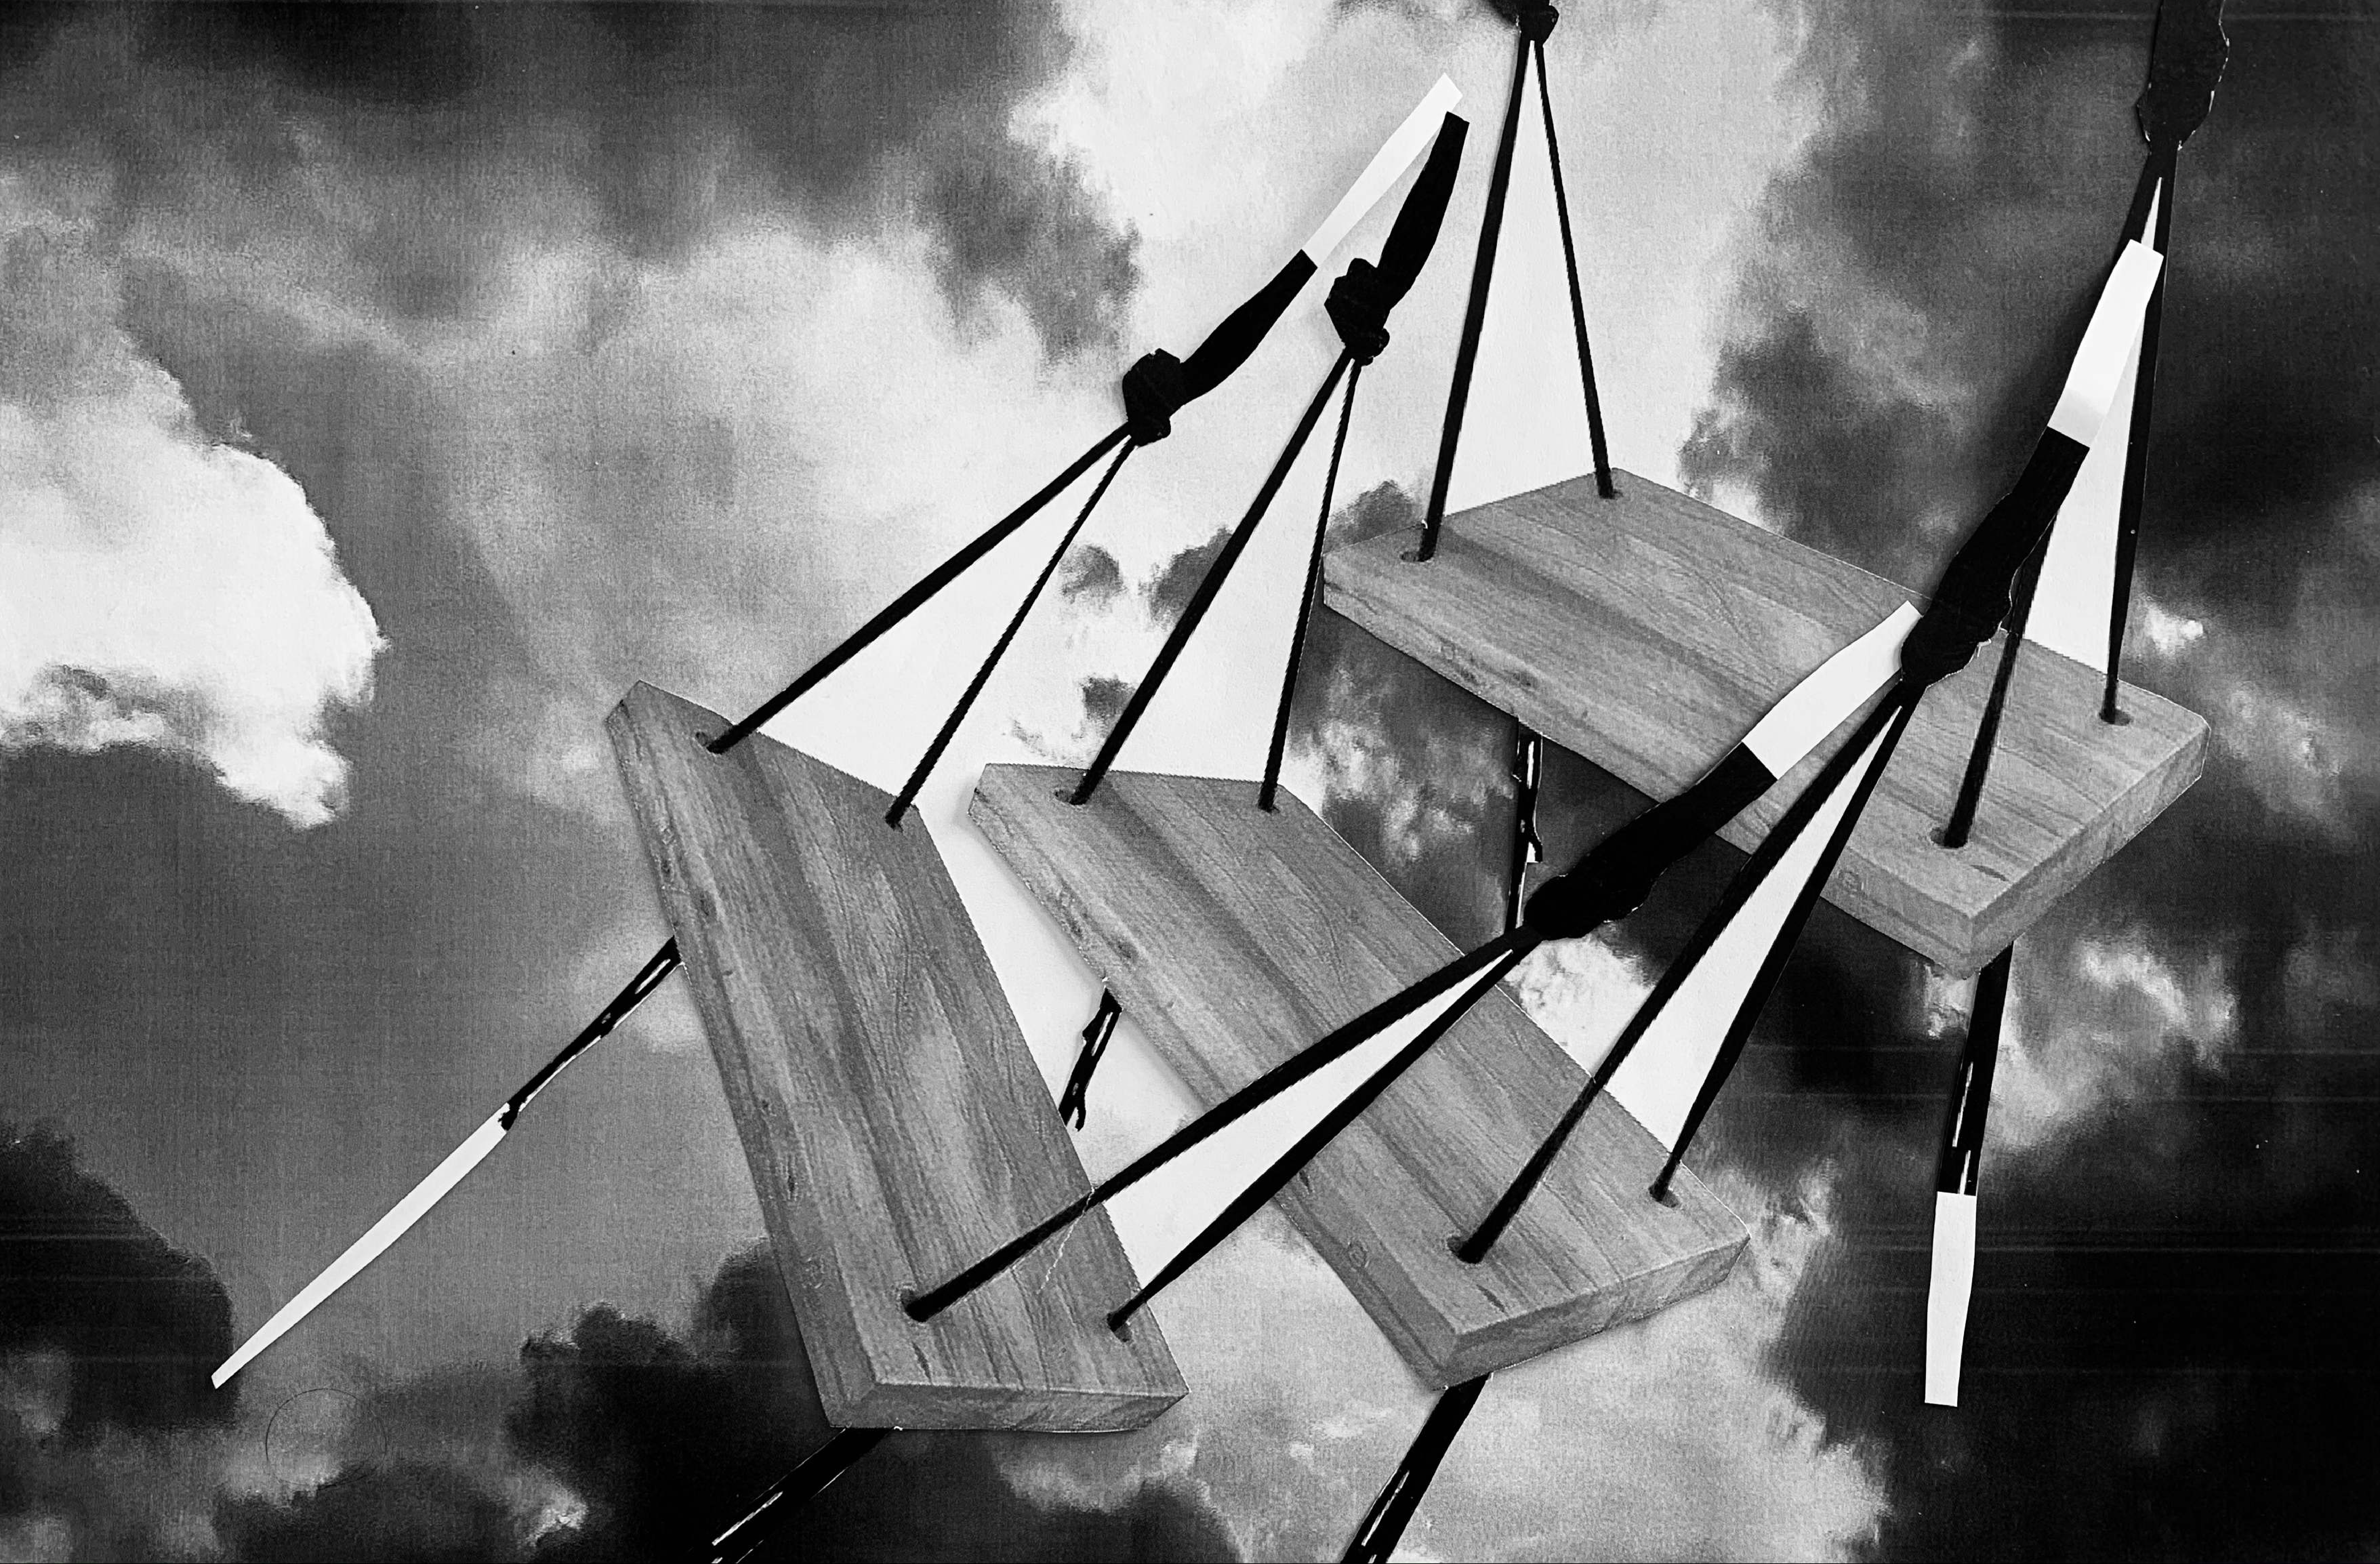
\includegraphics[width=2.83748in,height=1.86486in]{figuras/estudo-projecao-exlusao-matizes.pdf.compressed.pdf}

	\figurenote{Fonte: \archivef}
\end{minipage}
\end{figure}

A mocinha do Fragonard ficou de fora desta pintura, porque não tinha
definida a forma como entraria no trabalho. Decidi então voltar a usar
o rosa (o mesmo da pintura \emph{Carregando a mala}) na imprimatura,
para fazer um céu. Escolhi como referência para esta pintura o trabalho
de Will Cotton (1965), que possuía corpos bem fantasiosos sobrepostos à
imagem de um céu. O título desta pintura ficou assim: \emph{No quintal
	da vovó tinha um balanço}.

\begin{figure}
\begin{minipage}{.6\linewidth}
	\caption{\artname{\odette}{No quintal da vovó tinha um balanço}{2021}}%
	\label{odette-quintal-vovo-tinha-balanco-2021}
	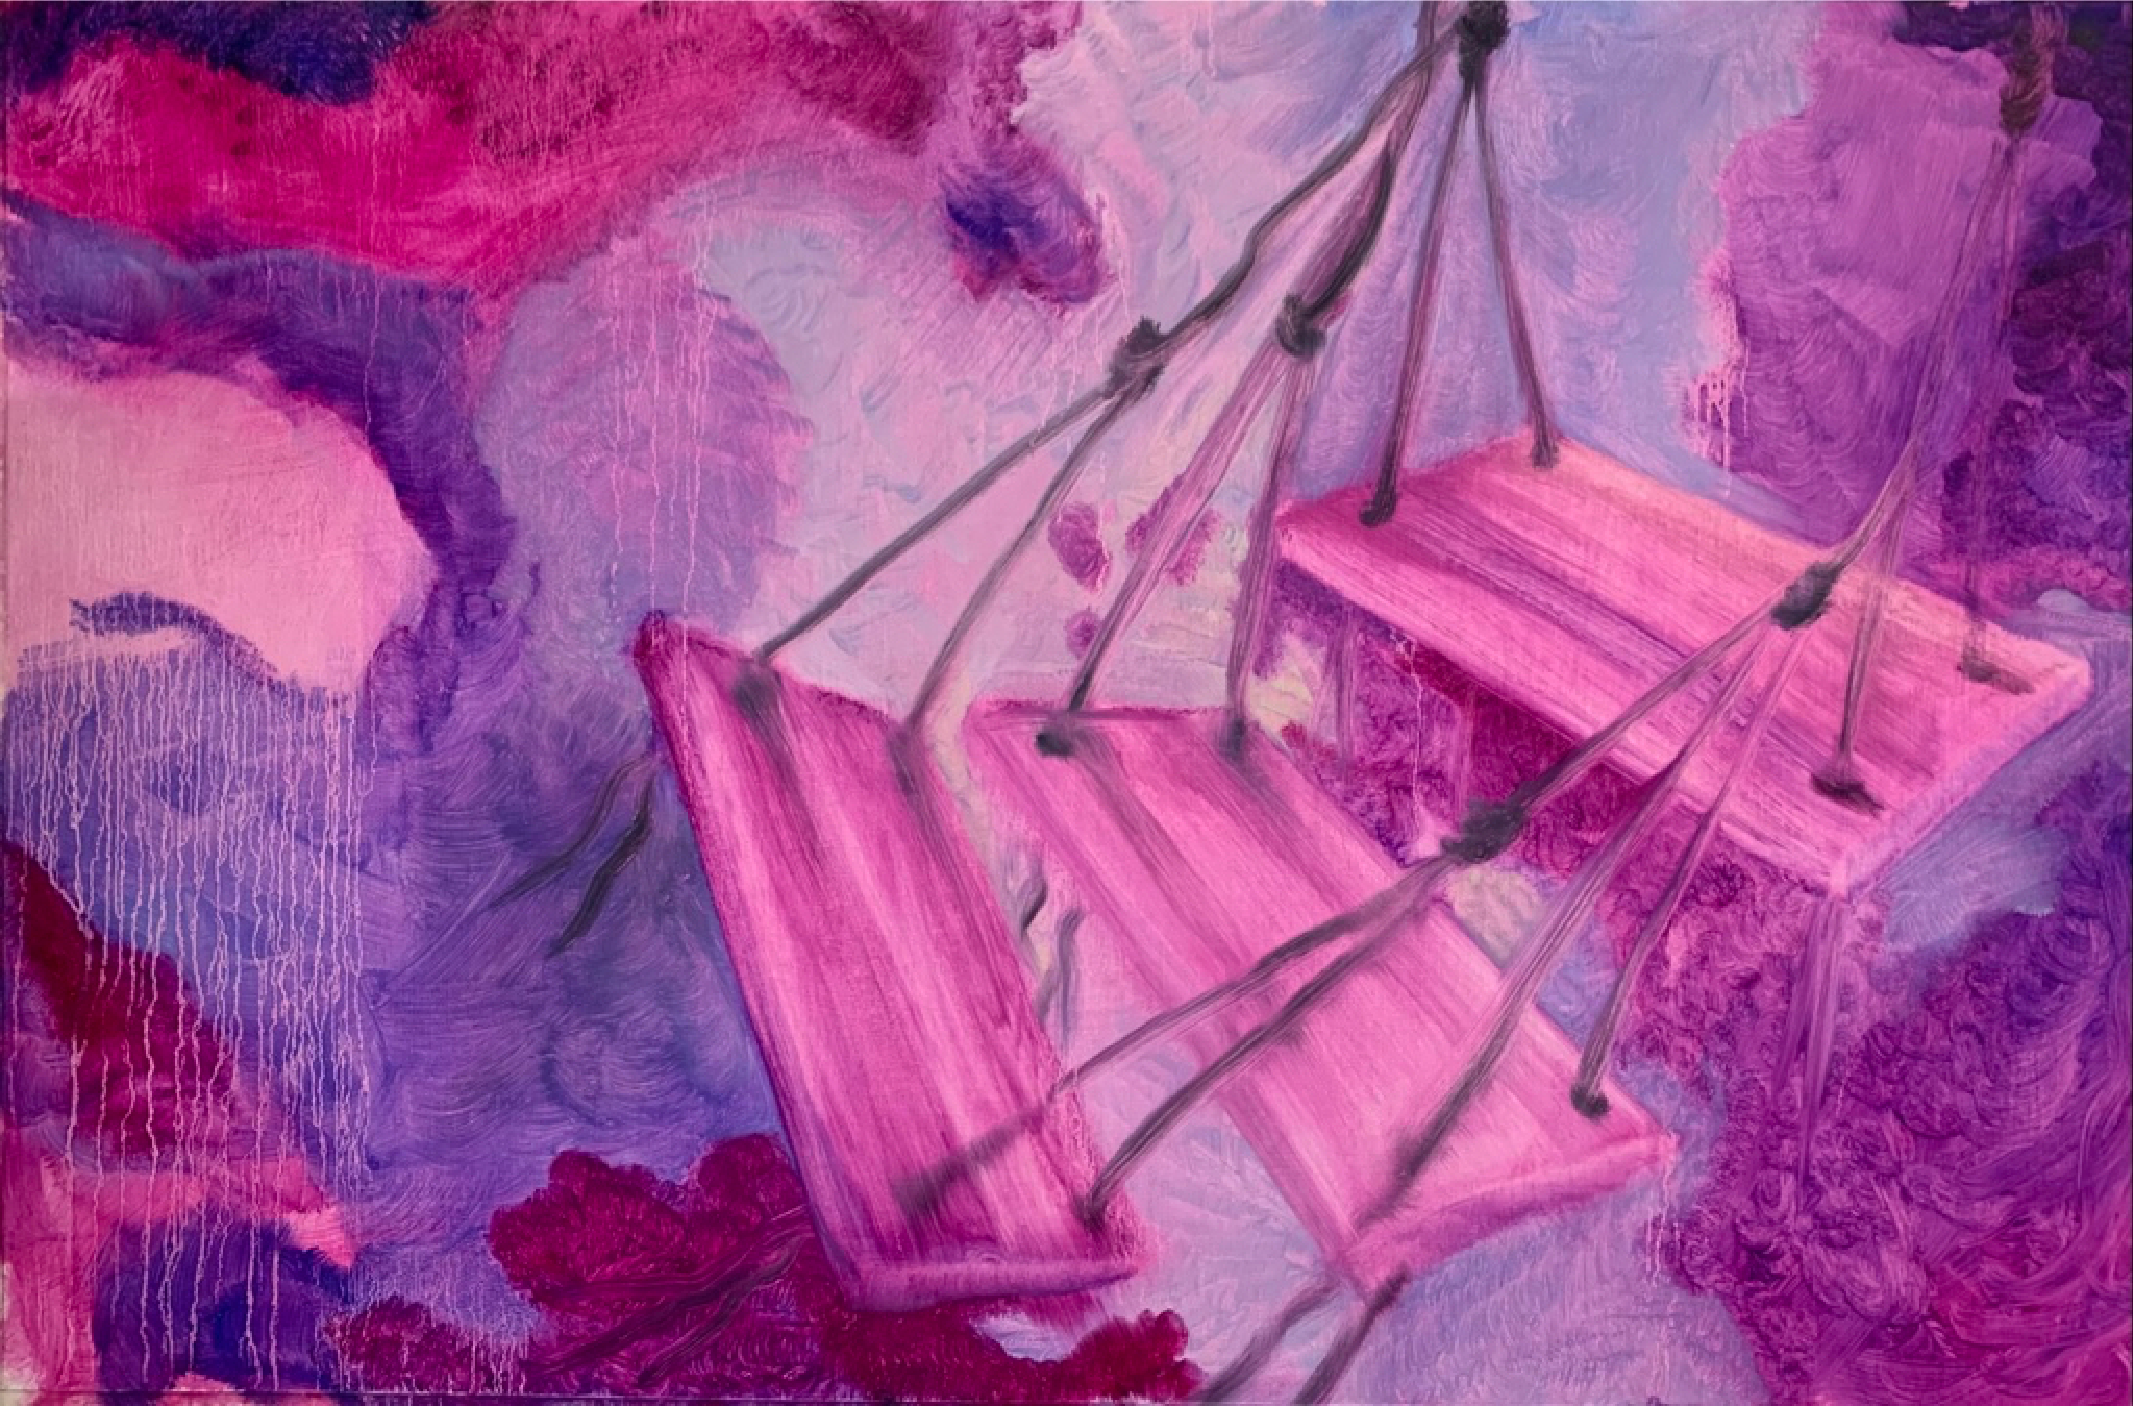
\includegraphics[width=3.38543in,height=2.229in]{figuras/odette-quintal-vovo-tinha-balanco-2021.pdf.compressed.pdf}
	\figurenote{\series{Movimento de câmera}. \oleolinho  \artsize{47x72x4}. Foto da autora}
\end{minipage}\hfill
\begin{minipage}{.3\linewidth}
	\caption{\artname{Will Cotton}{Fairy Floss}{2009--2010}}
	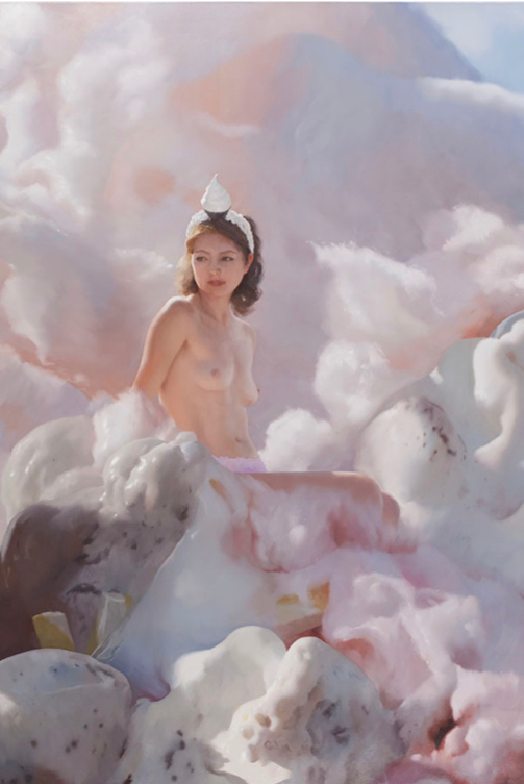
\includegraphics[height=2.229in]{figuras/cotton-fairy-floss.pdf.compressed.pdf}
	\figurenote{Fonte: \hiperlink{www.willcotton.com/paintings/2009.html}{Sítio de Will Cotton}}
\end{minipage}
\end{figure}

Experimentei formas distintas de pintar a mocinha, inclusive sobre
recortes em tecido, a fim de chegar a alguma possibilidade de inclusão
deste elemento na série do balanço. Por se tratar de uma figura humana
muito detalhada, me sentia pouco à vontade para jogá-la diretamente na
composição.

\pagebreak

A possibilidade de explorar o Movimento sequencial em repetição do
cinema me atraía, e assim nasceu a série \emph{Sapatinhos Voadores},
que se mescla com o projeto \emph{Balanço}. Fiz novos estudos através
da colagem, criando o díptico \emph{Elas levantam a saia e chutam},
onde recorto as figuras e pinto a óleo sobre tecido de algodão brocado.

\begin{figure}
  \flushright
\begin{minipage}{3.9in}
	\caption{\artname{\odette}{Elas levantam a saia e chutam}{2021}}
	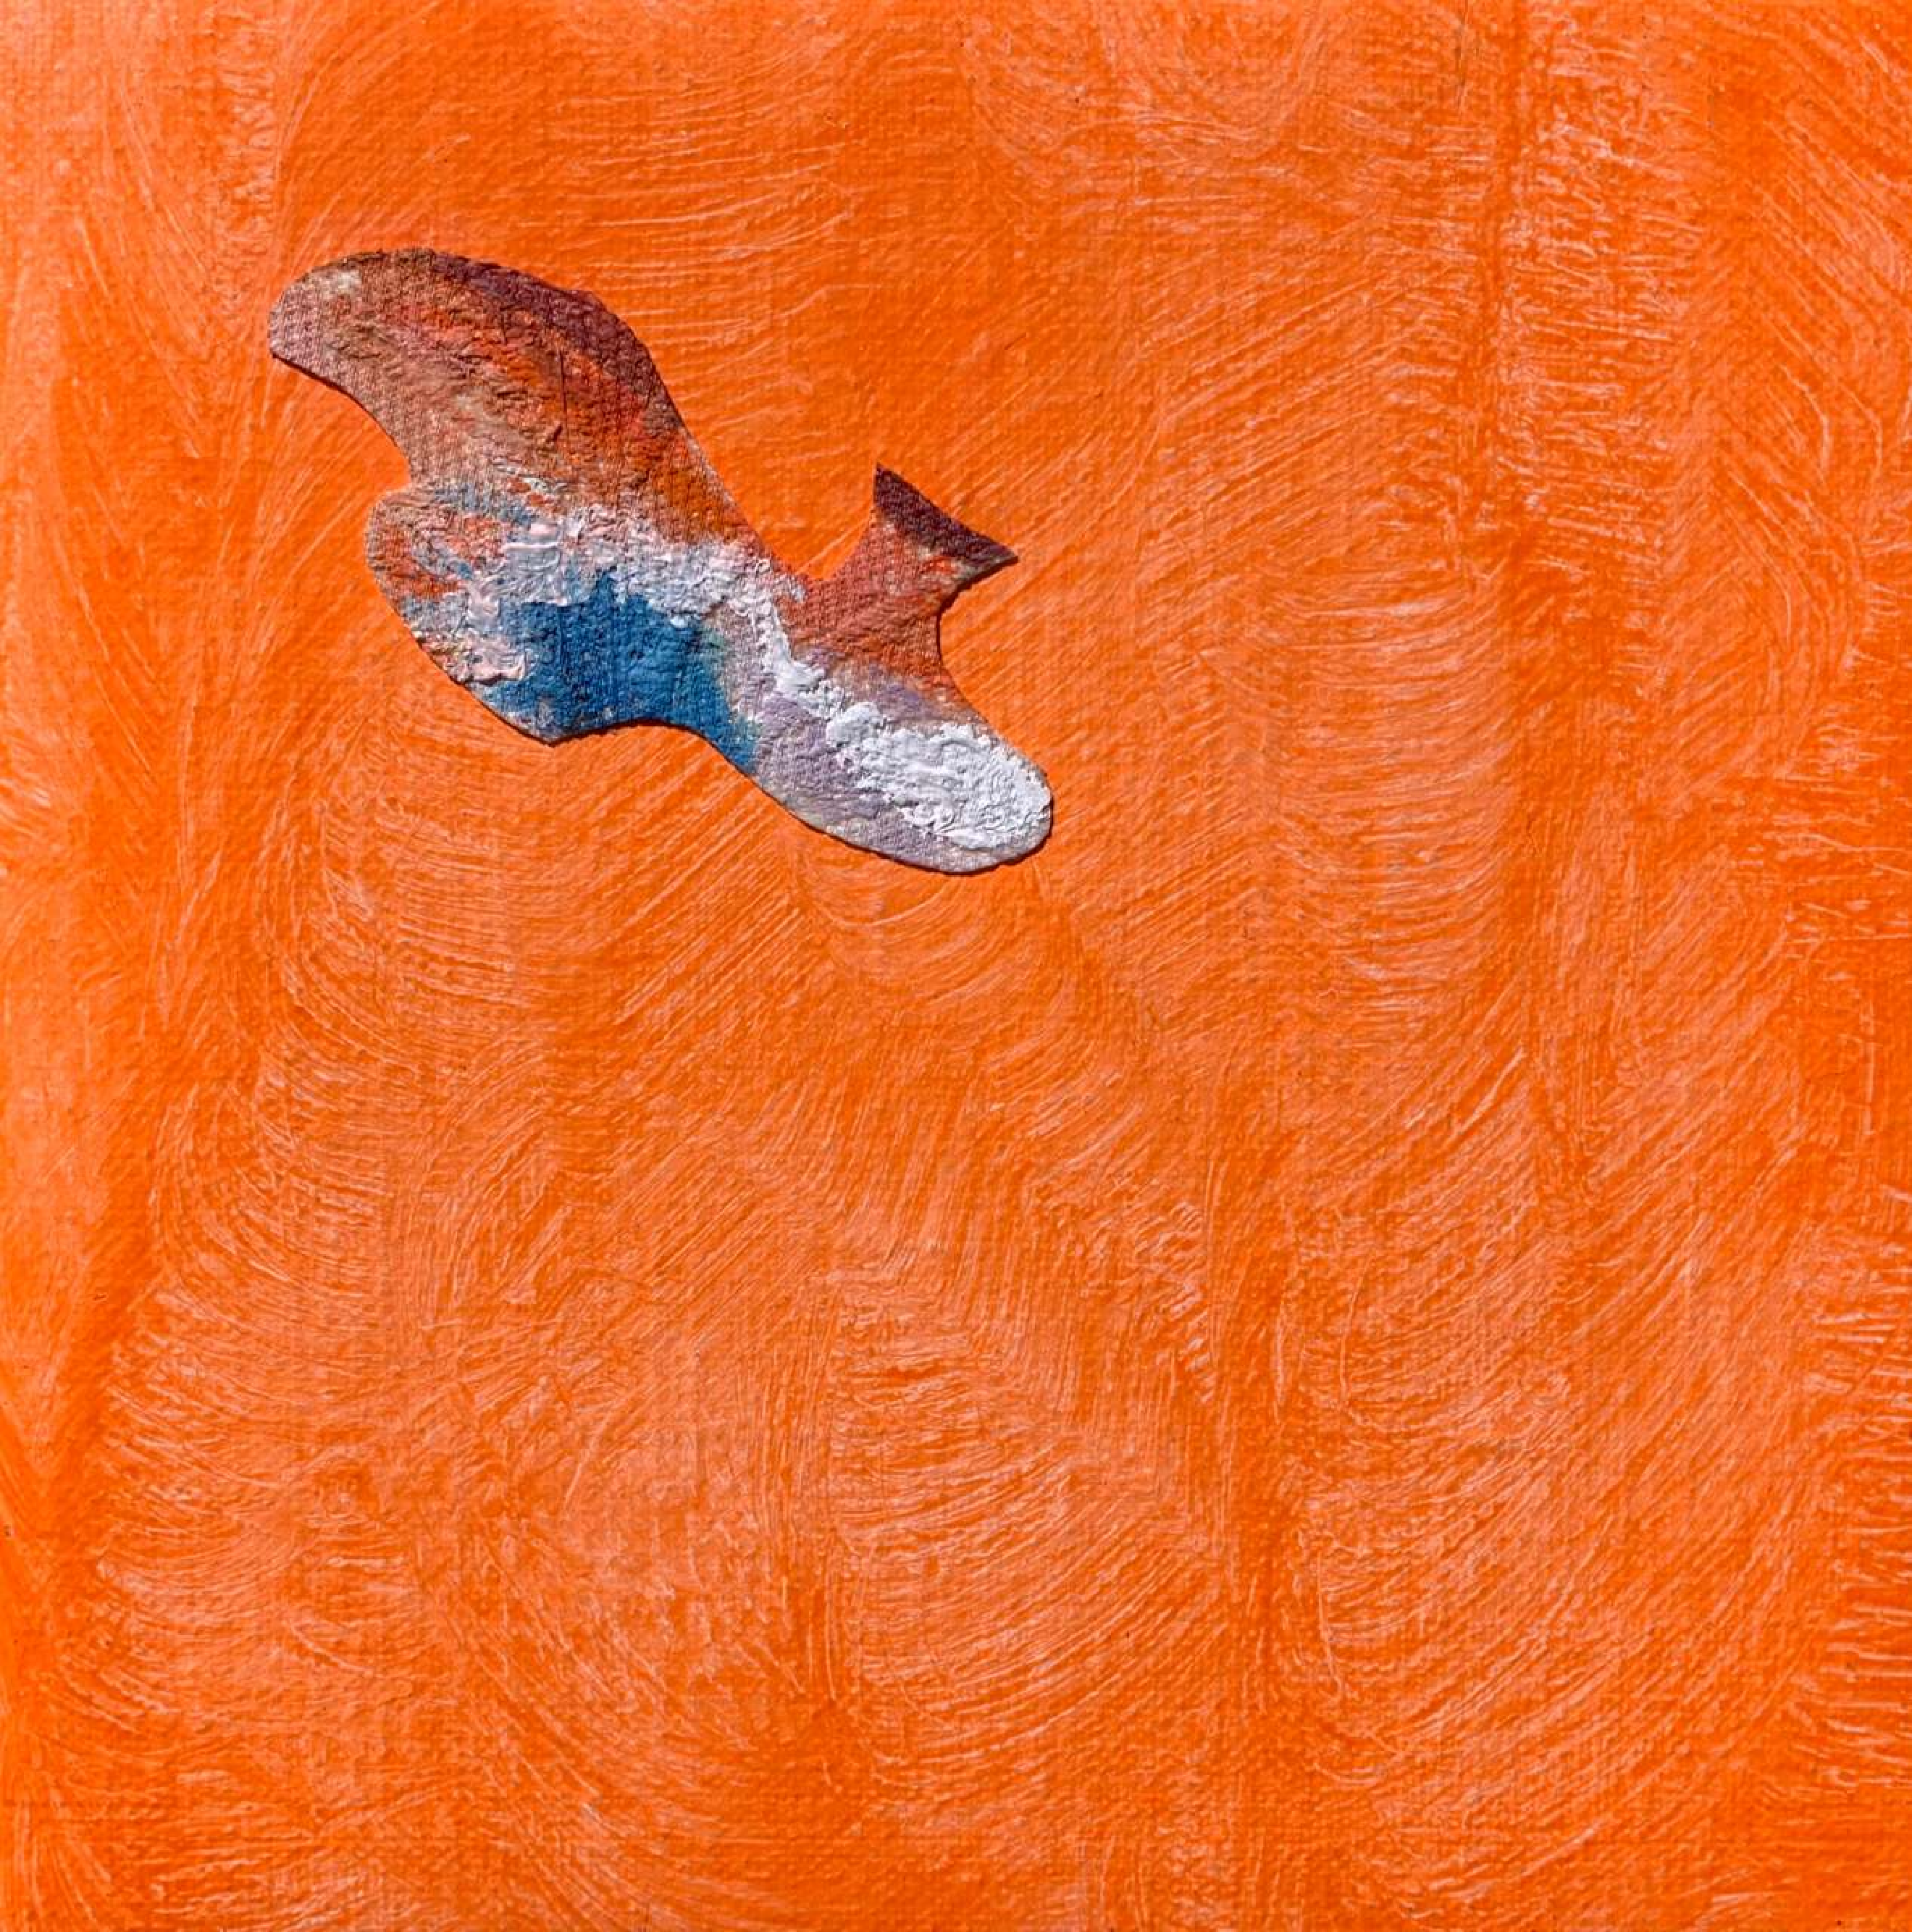
\includegraphics[width=1.85432in,height=1.86598in]{figuras/odette-elas-levantam-saia-chutam-esquerda.pdf.compressed.pdf}
	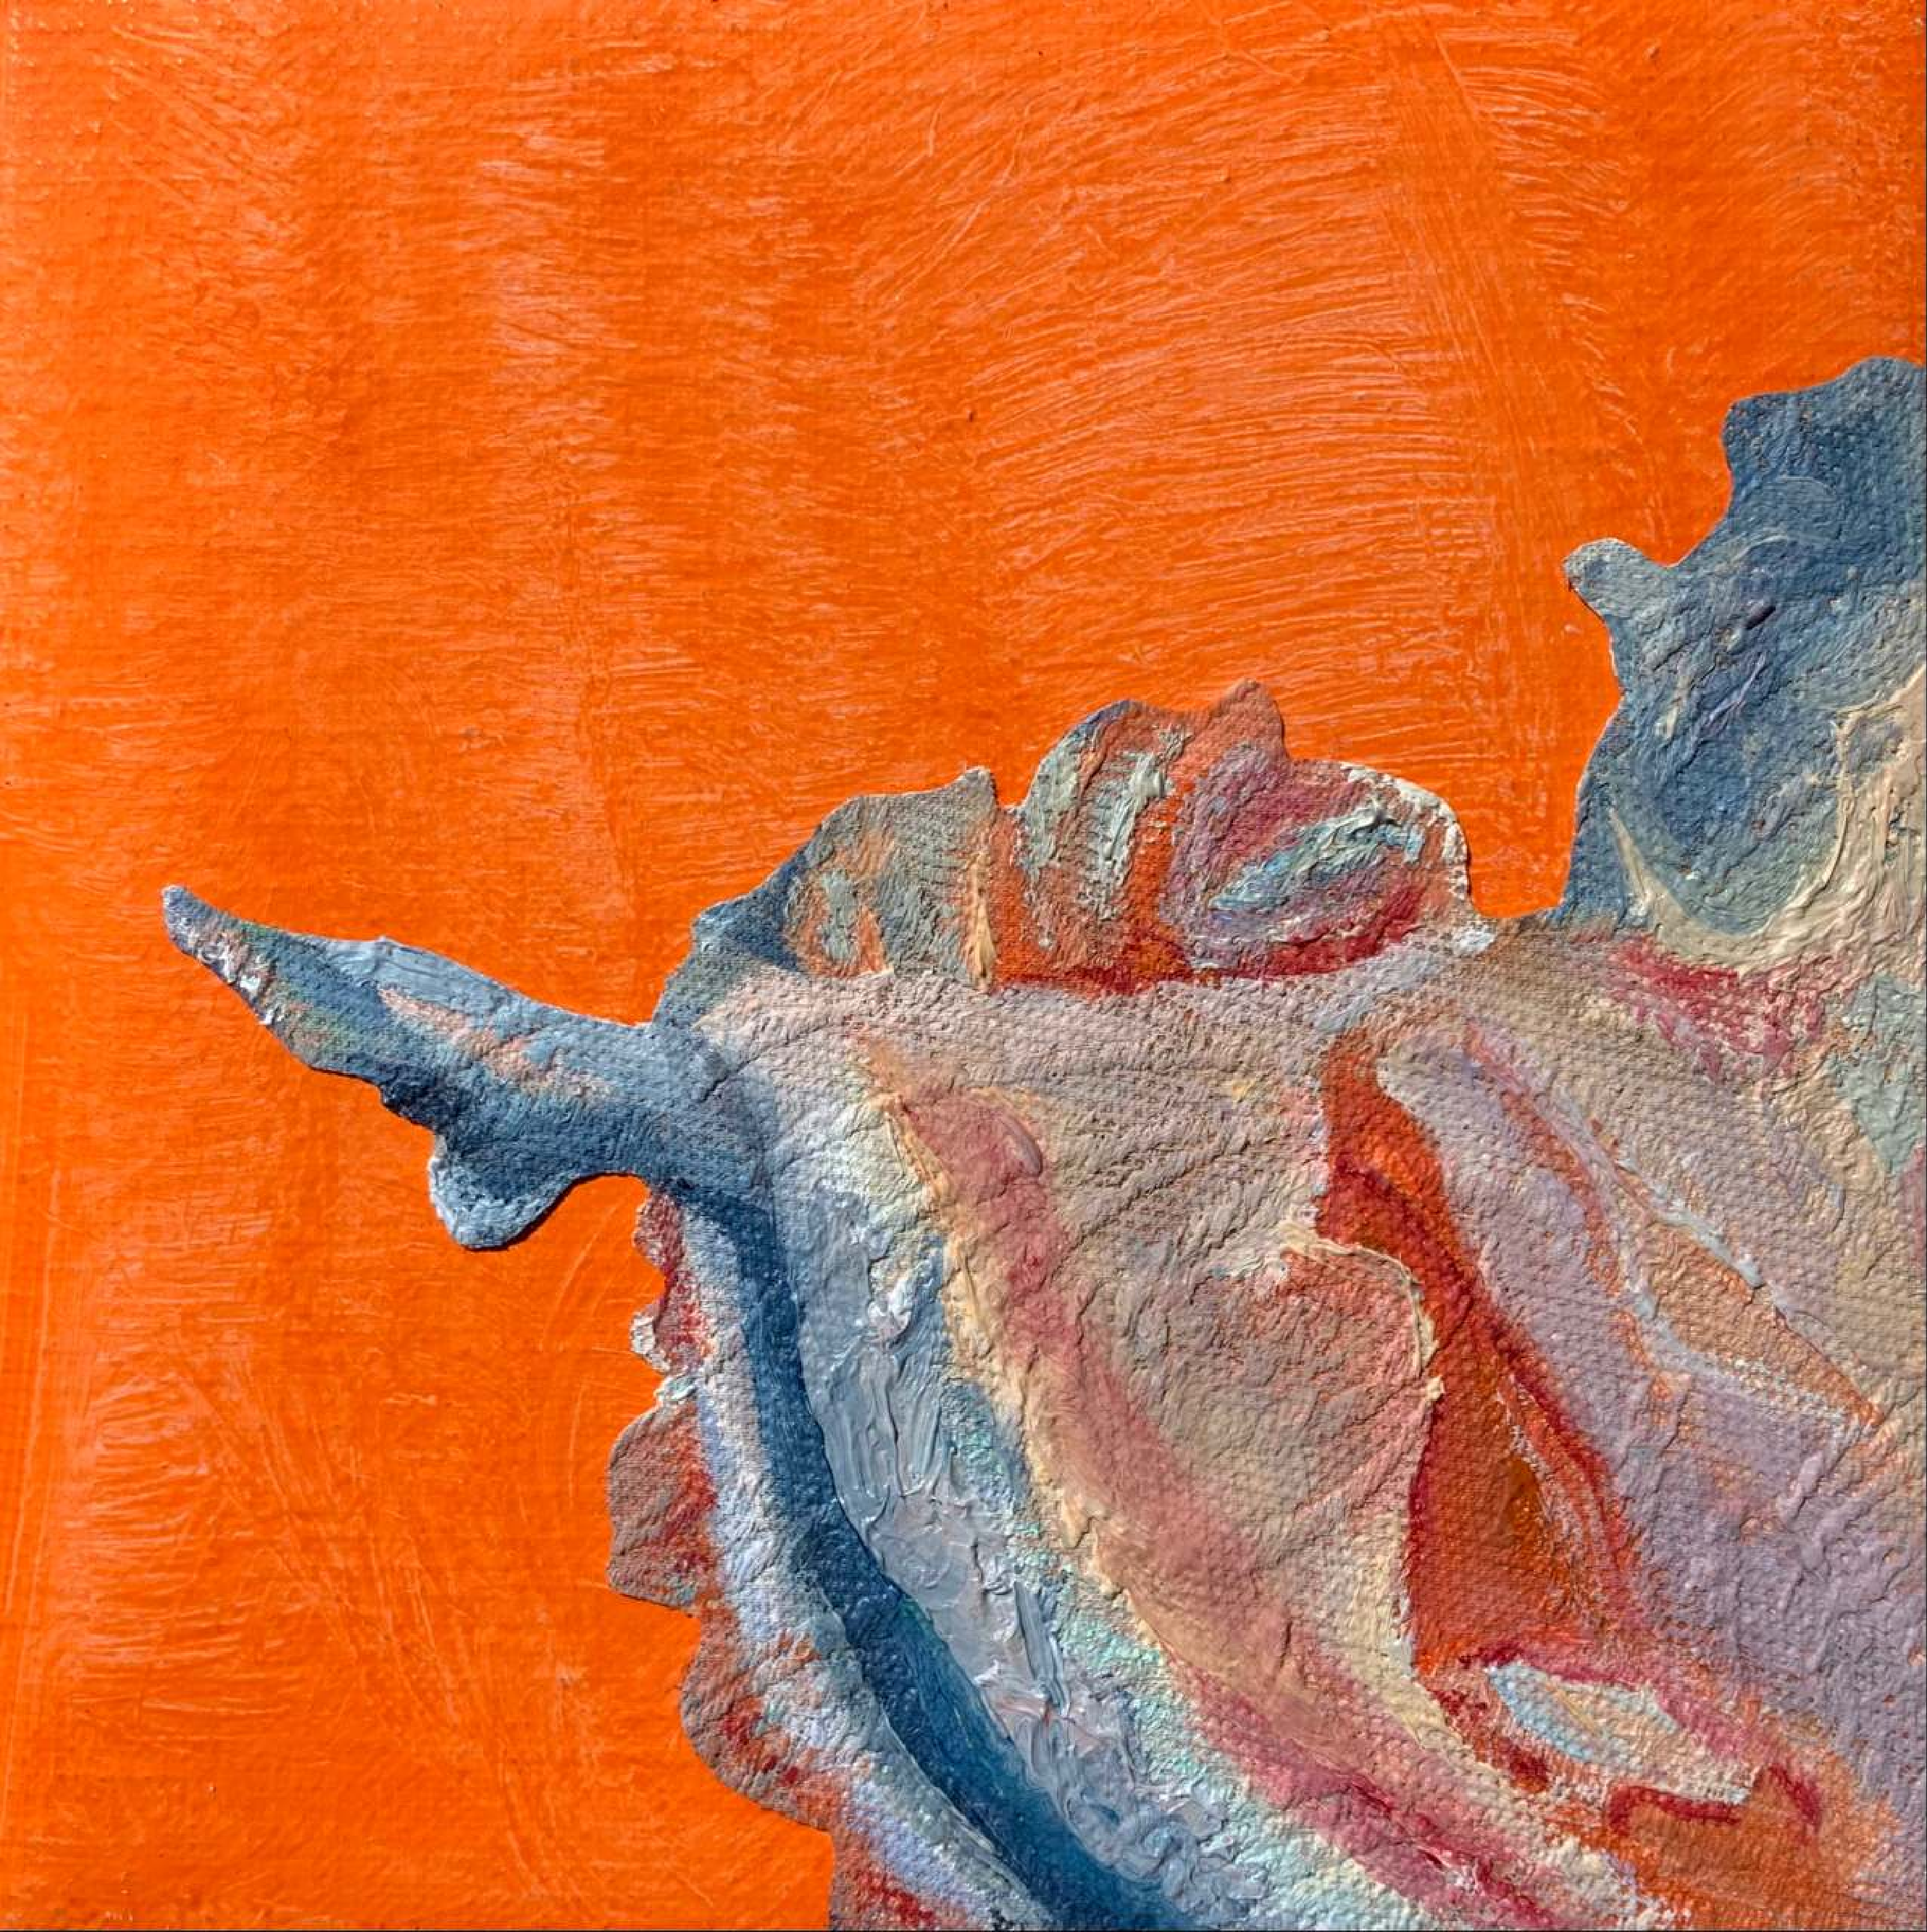
\includegraphics[width=1.85903in,height=1.86339in]{figuras/odette-elas-levantam-saia-chutam-direita.pdf.compressed.pdf}
	\figurenote{\series{Sapatinhos voadores}. Colagem e Óleo sobre têxtil e linho. \artsize{15x30x3.5}. Foto da autora}
\end{minipage}
\end{figure}

O projeto atual, \emph{Olhar do cinema}, inicia logo após a realização
da pintura de um balanço, intitulada \emph{Memória em Inércia}, no qual
eu me inspiro no movimento do cinema, como uma espécie de metáfora
invertida.

\begin{figure}
	\caption{\artname{\odette}{Memória em
			inércia}{2021}}

	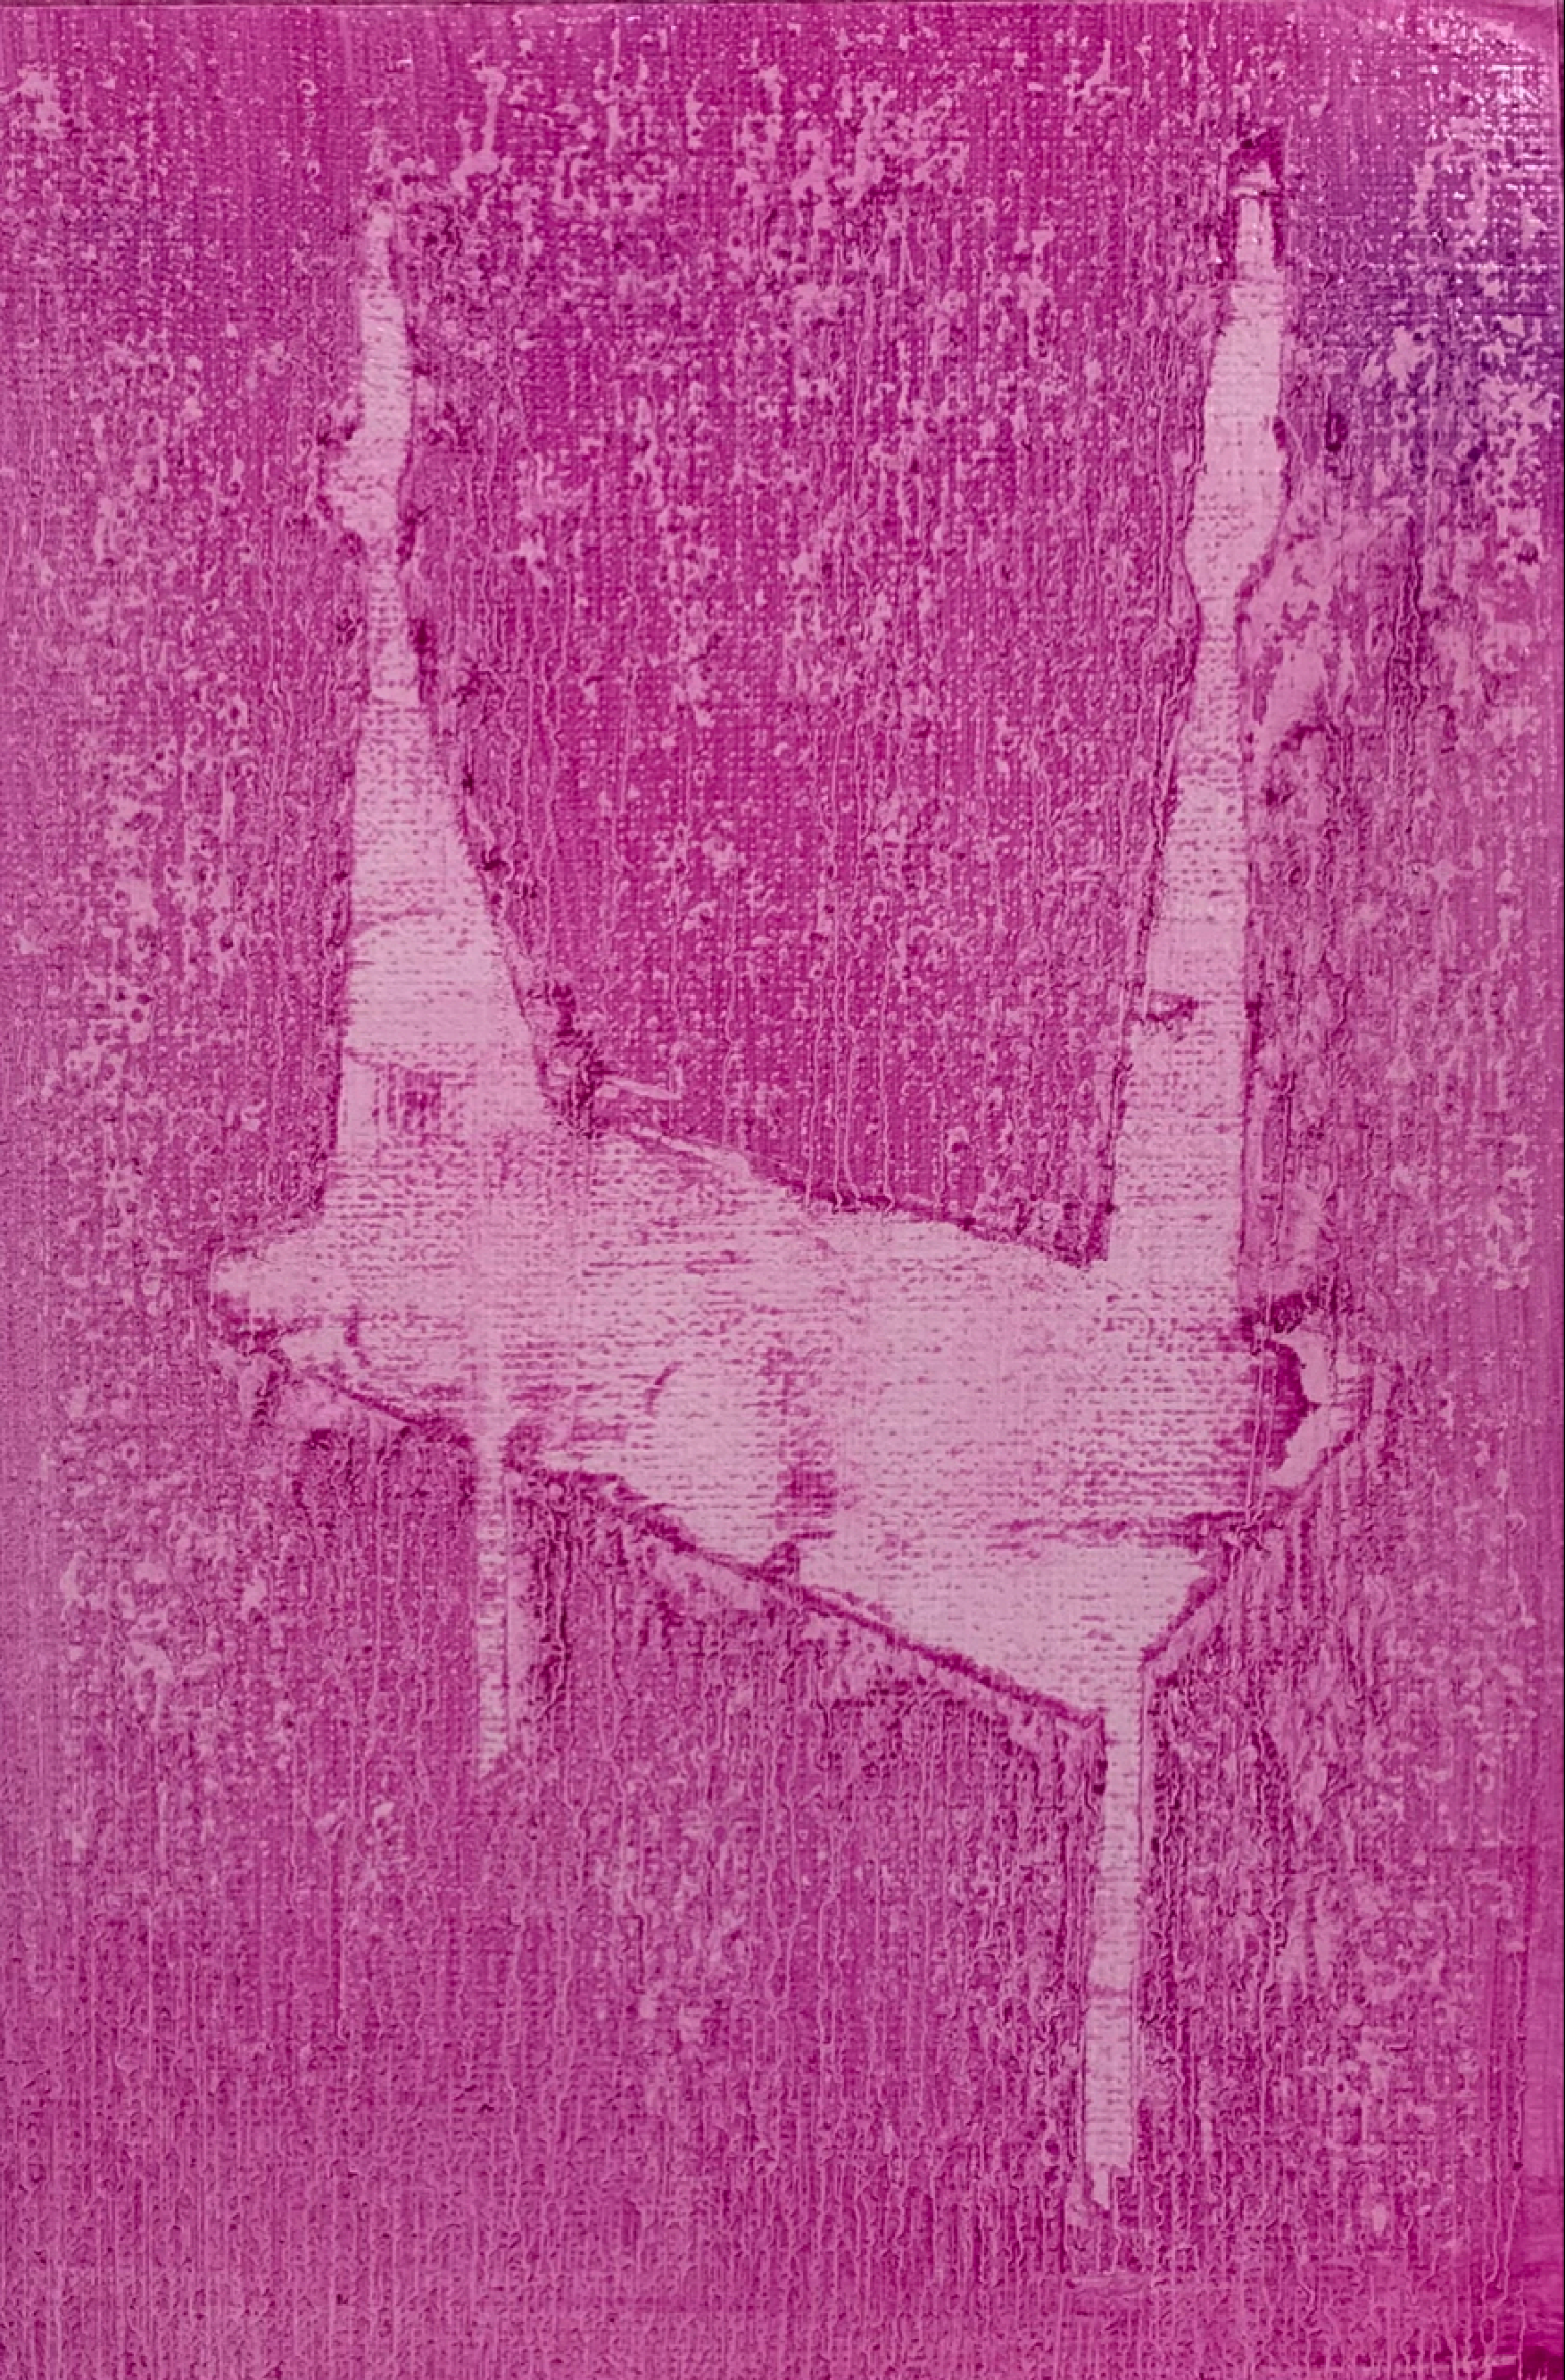
\includegraphics[width=1.85297in,height=2.81553in]{figuras/boudet-memoria-inercia-2021.pdf.compressed.pdf}
	\figurenote{\series{Movimento de câmera}. \oleolinho. \artsize{30x20x3.5}. Foto da autora}
\end{figure}

\pagebreak

Tratando especificamente deste projeto, de suas cores e de frames de
filmes ícones da história do cinema, passo a descrever, a partir de
agora, as primeiras pinturas que se relacionam diretamente com esta
temática.

Os enquadramentos, as angulações propostas pelo posicionamento da
câmera de filmar sempre me atraíram. O ponto de vista, para
\textcite{jullier2009lendo} é tido como o parâmetro mais importante ao
nível do plano cinematográfico, e tem por princípio básico a
localização estratégica da câmera em relação ao cenário e seus
elementos estáticos e em movimento. Com relação ao espaço
tridimensional, o operador de câmera precisa fazer três escolhas
topográficas: o comprimento do eixo da objetiva (próximo ou distante,
close-up ou plano geral); na lateralidade (centralizado ou
descentralizado); e na verticalidade (câmera alta, câmera baixa, câmera
alta total, câmera baixa total, frontalidade e desenquadramento.
Entretanto, faz mais sentido flexibilizar estas posições de comprimento
do eixo durante a montagem, ou seja, no nível da sequência. Desta forma
tem-se o plano médio que apresenta o sujeito em sua unidade (seja ela
humana, animal, vaso de flores, automóvel), o close-up (ou plano
detalhe e grande plano em lusitano) e o plano geral, que insere o
sujeito em seu ambiente. Além disto cabe ressaltar a gíria\footnote{
	Linguagem usada por determinado grupo, geralmente incompreensível para
	quem não pertence ao grupo e que serve também como meio de realçar a
	sua especificidade. \textbf{\enquote{gíria}}, in Dicionário Priberam da
	Língua Portuguesa \textins{em linha}, 2008-2020,
	\hiperlink{https://dicionario.priberam.org/g\%25C3\%25ADria}{{https://dicionario.priberam.org/g\%C3\%ADria}}
	(consultado em 11 de janeiro de 2022).} do operador de câmera, que
preconiza um mínimo de \emph{ar}, em cima e embaixo dos sujeitos. Na
lateralidade existe a questão da centralização e descentralização, que
pode respeitar ou não a regra dos três terços, derivada da pintura. Na
verticalidade o eixo da objetiva aponta para o centro do sujeito, desce
na sua direção quando a câmera está alta ou sobe na direção do sujeito
quando a câmera está baixa. Quando o ângulo entre o plano do chão e o
eixo da objetiva se aproxima de 90º graus, fala-se em \emph{câmera alta
	total} ou \emph{câmera baixa total.} Por fim a frontalidade do
enquadramento e a busca pelo paralelismo no final de uma panorâmica
deveriam ser levados em conta pelo diretor de fotografia %
\parencite[22-28]{jullier2009lendo}.

Percebemos, pela sistematização destes autores, que muitas das decisões
de posicionamento da câmera nas captações de imagem, guardam uma
intimidade grande com as que o pintor, no seu relacionamento com a tela
precisa tomar. Nesta perspectiva, o olhar da câmera poderia substituir
o gesto do pintor. E aqui podemos falar sobre o posicionamento do
pintor diante da tela. O corpo se movimenta, buscando a melhor forma de
iniciar o movimento, para aplicar o carvão, o pigmento, a tinta ou
qualquer outro tipo de matéria que se possa tratar na pintura. Uma
dança acontece entre a imagem mental e o impulso que alcança o objeto.
Aproximações e afastamentos, necessários à visualização do todo e do
pormenor da composição também acontecem, ora mais despojadas, ora mais
intimistas, nas tentativas de ensaio, erro, tirar, pôr, riscar, afagar,
bater, secar e deixar escorrer. Seja com a tela na forma vertical,
horizontal à moda de \emph{Pollock}, seja nos planejamentos de direção
cromática, dentro do quadro. As marcações, medidas que os fotógrafos de
câmera fazem antes do início do filme, se equivalem aos esboços que se
utilizam tanto de linhas feitas com carvão, fita-crepe, pincéis, giz, e
como estratégia cada vez mais usada por pintores contemporâneos, como o
uso do projetor.

\begin{figure}
  \begin{minipage}[b]{.475\linewidth}
	\caption{\artname{\odette}{Eu quero ir}{2020}}%
	\label{boudet-eu-quero-ir-2020}

	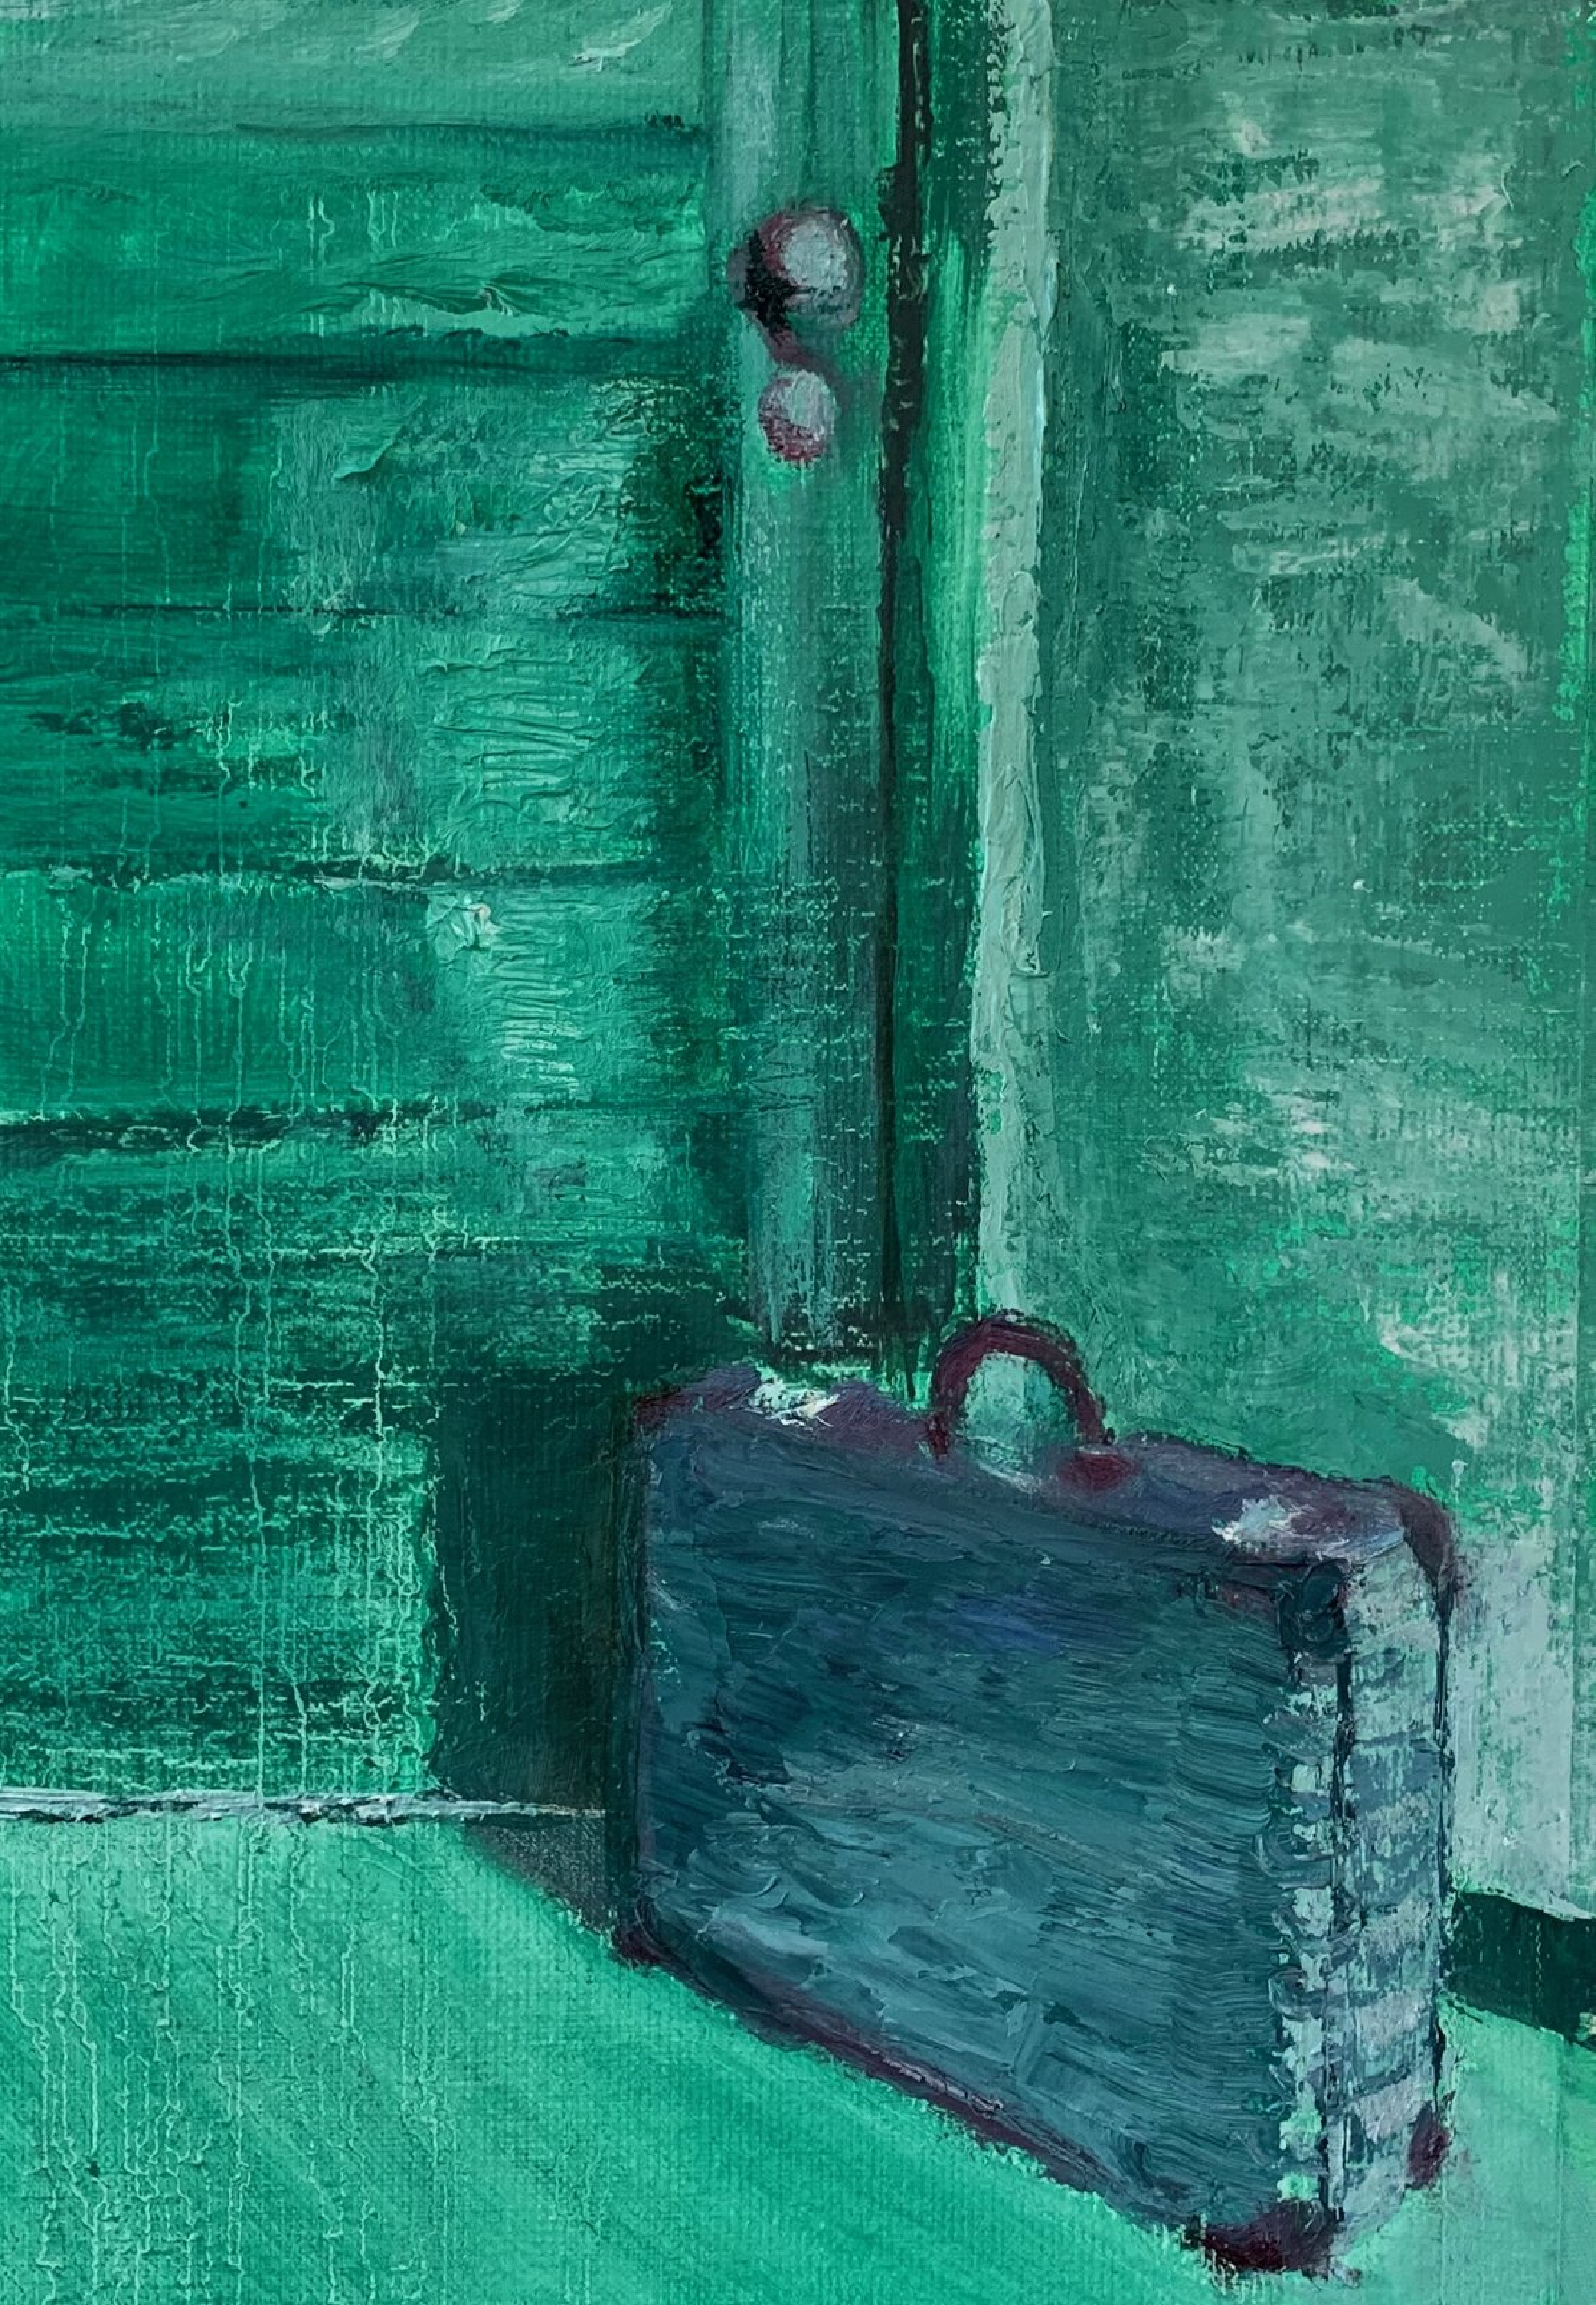
\includegraphics[width=.8\linewidth]{figuras/boudet-eu-queri-ir-2020.pdf.compressed.pdf}
	\figurenote{\series{Me leva}. \oleolinho. \artsize{30x20x4}. Foto da autora.}
\end{minipage}\hfill
\begin{minipage}[b]{.475\linewidth}
	\caption{\artname{\odette}{Contre plongée}{2020}}%
	\label{boudet-contre-plogee-2020}

	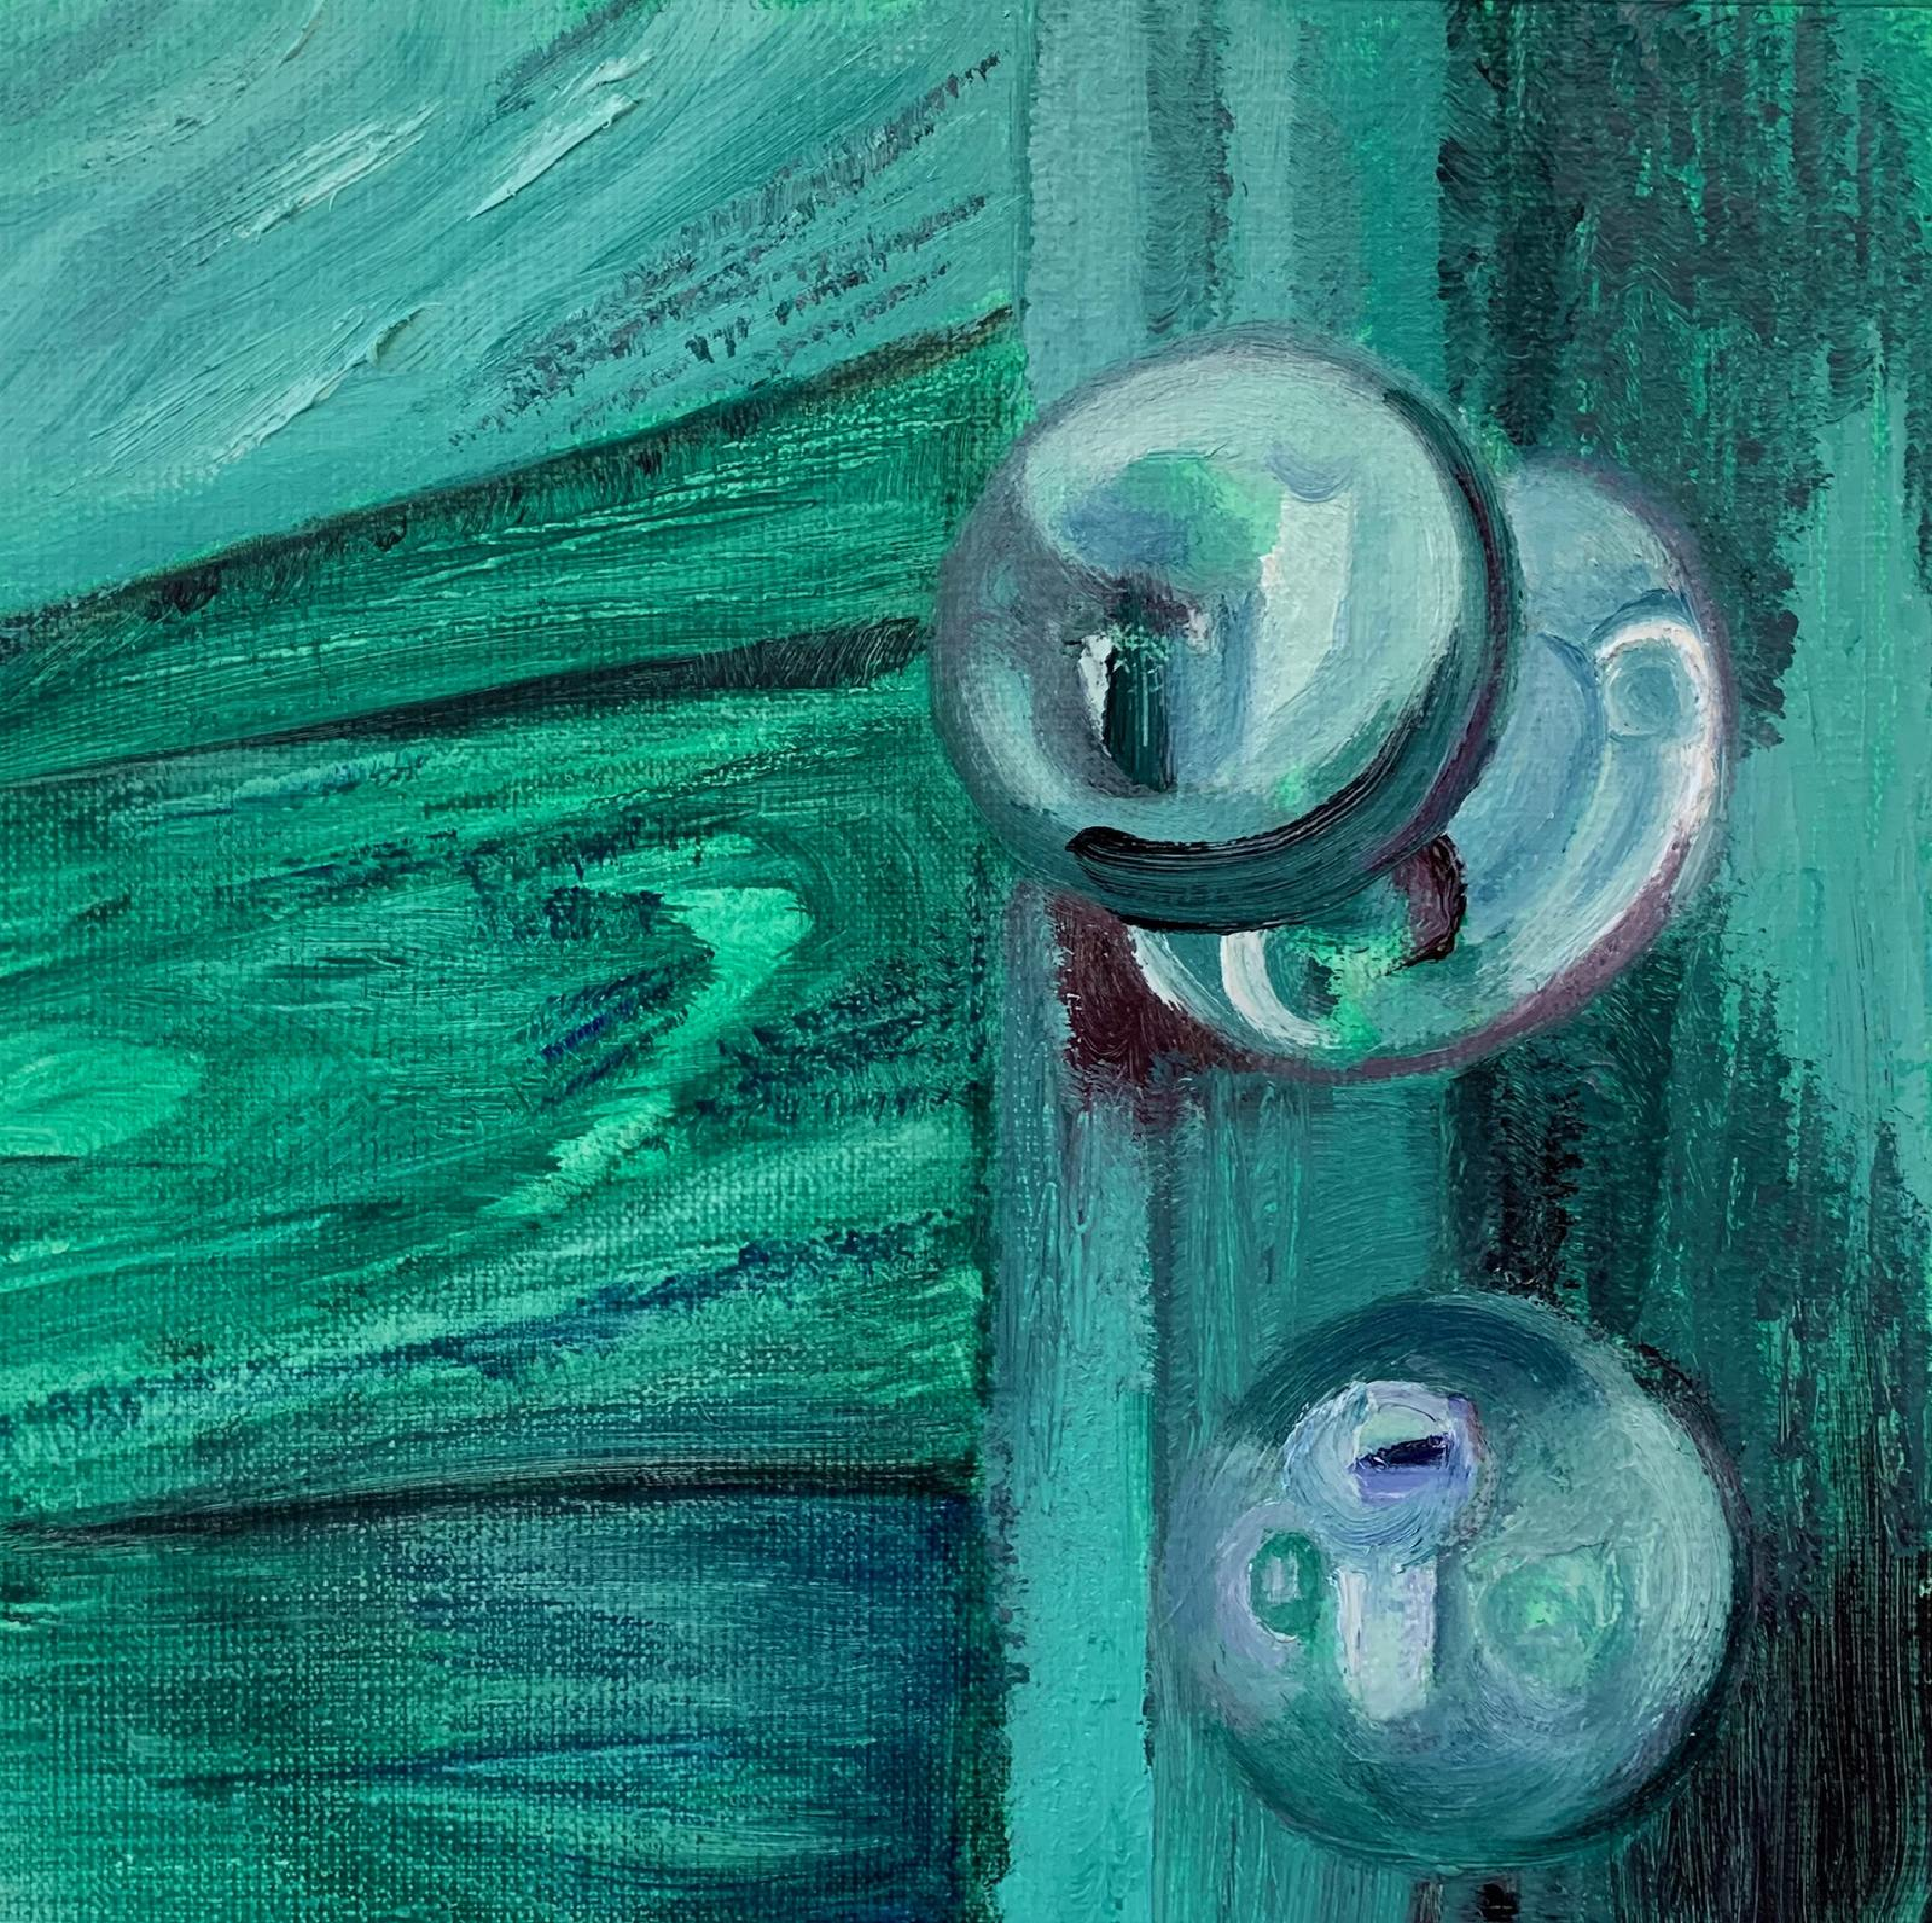
\includegraphics[width=.8\linewidth]{figuras/boudet-contre-plogee2020.pdf.compressed.pdf}
	\figurenote{\series{Me leva}. \oleolinho. \artsize{20x20x4}. Foto da autora}
\end{minipage}
\end{figure}

O \emph{plongée}, que significa mergulho, foi pensado para relacionar
dois trabalhos: \emph{Eu quero ir, 2020}, e \emph{Contre-plongée,
2020} (\cref{boudet-eu-quero-ir-2020,boudet-contre-plogee-2020}). O mergulho que a câmera do cinema dá ao enquadrar uma
determinada cena e a ideia de campo/contracampo inspiraram a
apresentação destas duas pinturas \emph{que se olham}. A mala se coloca
em \emph{contra-plongée} e lança um olhar para a fechadura da porta.

Quando realizei a pintura \emph{Na casa da vovó tinha um balanço}
(\cref{odette-quintal-vovo-tinha-balanco-2021}) minha intenção era
refletir sobre o Movimento de ir e vir, como em um pêndulo. Muito tempo
depois, analisando as pinturas \emph{Eu quero ir}
(\cref{boudet-eu-quero-ir-2020}) e \emph{Contre-plongée}
(\cref{boudet-contre-plogee-2020}), compreendi a relação entre uma
imagem afetiva e o ponto de vista habituado à intermediação de uma
câmera. Eu pesquiso na pintura recortes na composição da imagem
fotográfica e a intermediação de uma câmera muitas vezes atravessa o
pensamento e o gesto. Compreender o mundo para mim é instaurar uma
imagem. Aquela que mesmo sem sabermos de que parte da memória vem,
precisa ser colocada diante de nós. Foi assim com o projeto Balanço.
Ele veio e só depois de algum tempo eu o enxerguei lá, em um
enquadramento plongée. \emph{Era o balanço no quintal da vovó, visto de
	cima da minha varanda.}

Criar um \emph{storyboard}, por meio da pintura também era e ainda é um
objetivo. No entanto, muito antes de construir uma narrativa, a
finalidade maior sempre foi experimentar técnicas e processos na
pintura. Realizei as pinturas \emph{Under the bed, 2021} (\cref{under-the-bed}) e
\emph{Rolamento suspenso, 2021} (\cref{rolamento-suspenso}) e criei a série \emph{Movimento de
	câmera}, imaginando a mala se movimentando e saindo debaixo da cama.
Dei seguimento a este grupo de trabalhos com a pintura \emph{Retrato na
parede, 2021} (\cref{retrato-na-parede}), onde as rodinhas da mala criam uma sombra sobre um fundo
branco.

A série intitulada \emph{Movimento de câmera} veio ao encontro dos
primeiros estudos para o Projeto \enquote{Olhar do cinema.} Foi a
partir desta série que apliquei uma metodologia que parte da
identificação dos principais interesses do artista, por meio de escolha
aleatória de figuras, paletas e padrões, caminhando para ideias de
esboços e trabalhos finalizados, que se desdobram em séries e projetos.

\newpage

\begin{figure}
  \begin{minipage}[b]{.3\linewidth}
  \caption{\artname{\odette}{Rolamento suspenso}{2021}.}\label{rolamento-suspenso}

  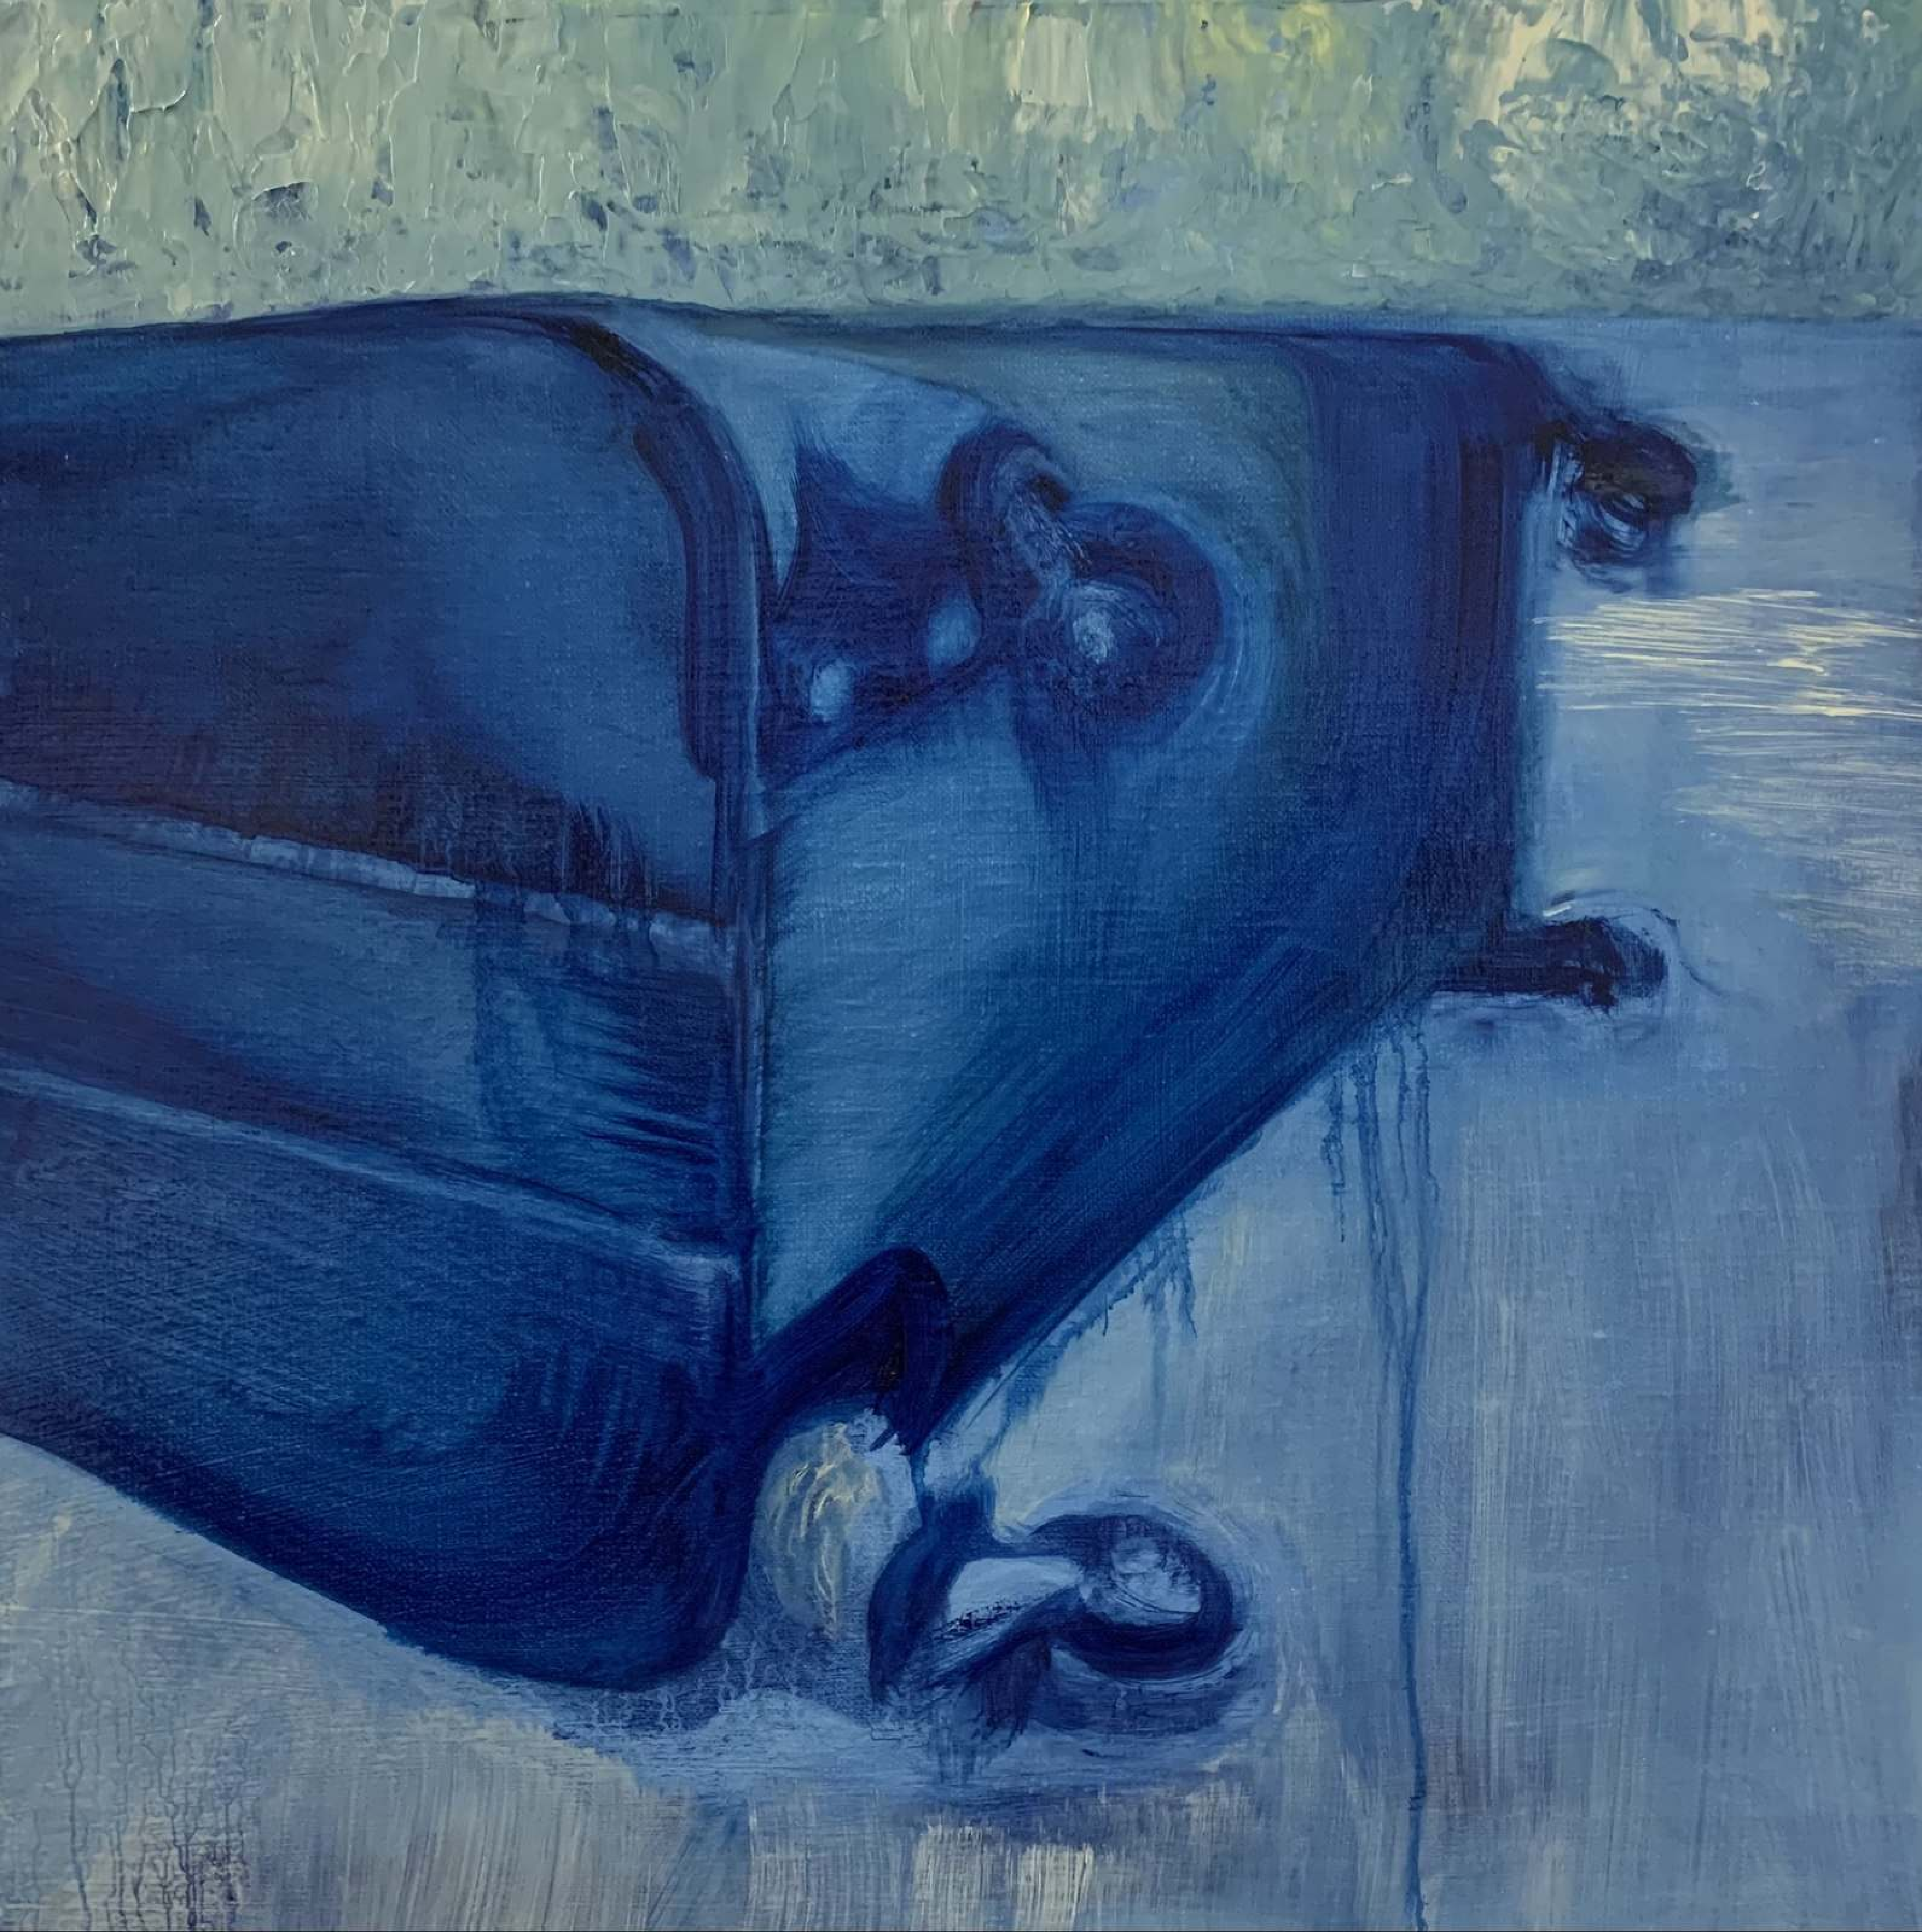
\includegraphics[width =.88\linewidth]{figuras/boudet-rolamento-suspenso-20201.pdf.compressed.pdf}
	\figurenote{\series{Movimento de câmera}. \oleolinho. \artsize{37.5x37.5x4}. \\ Foto da autora.}
\end{minipage}\hfill
\begin{minipage}[b]{.3\linewidth}
  \caption{\artname{\odette}{Under the bed}{2021}.}\label{under-the-bed}
	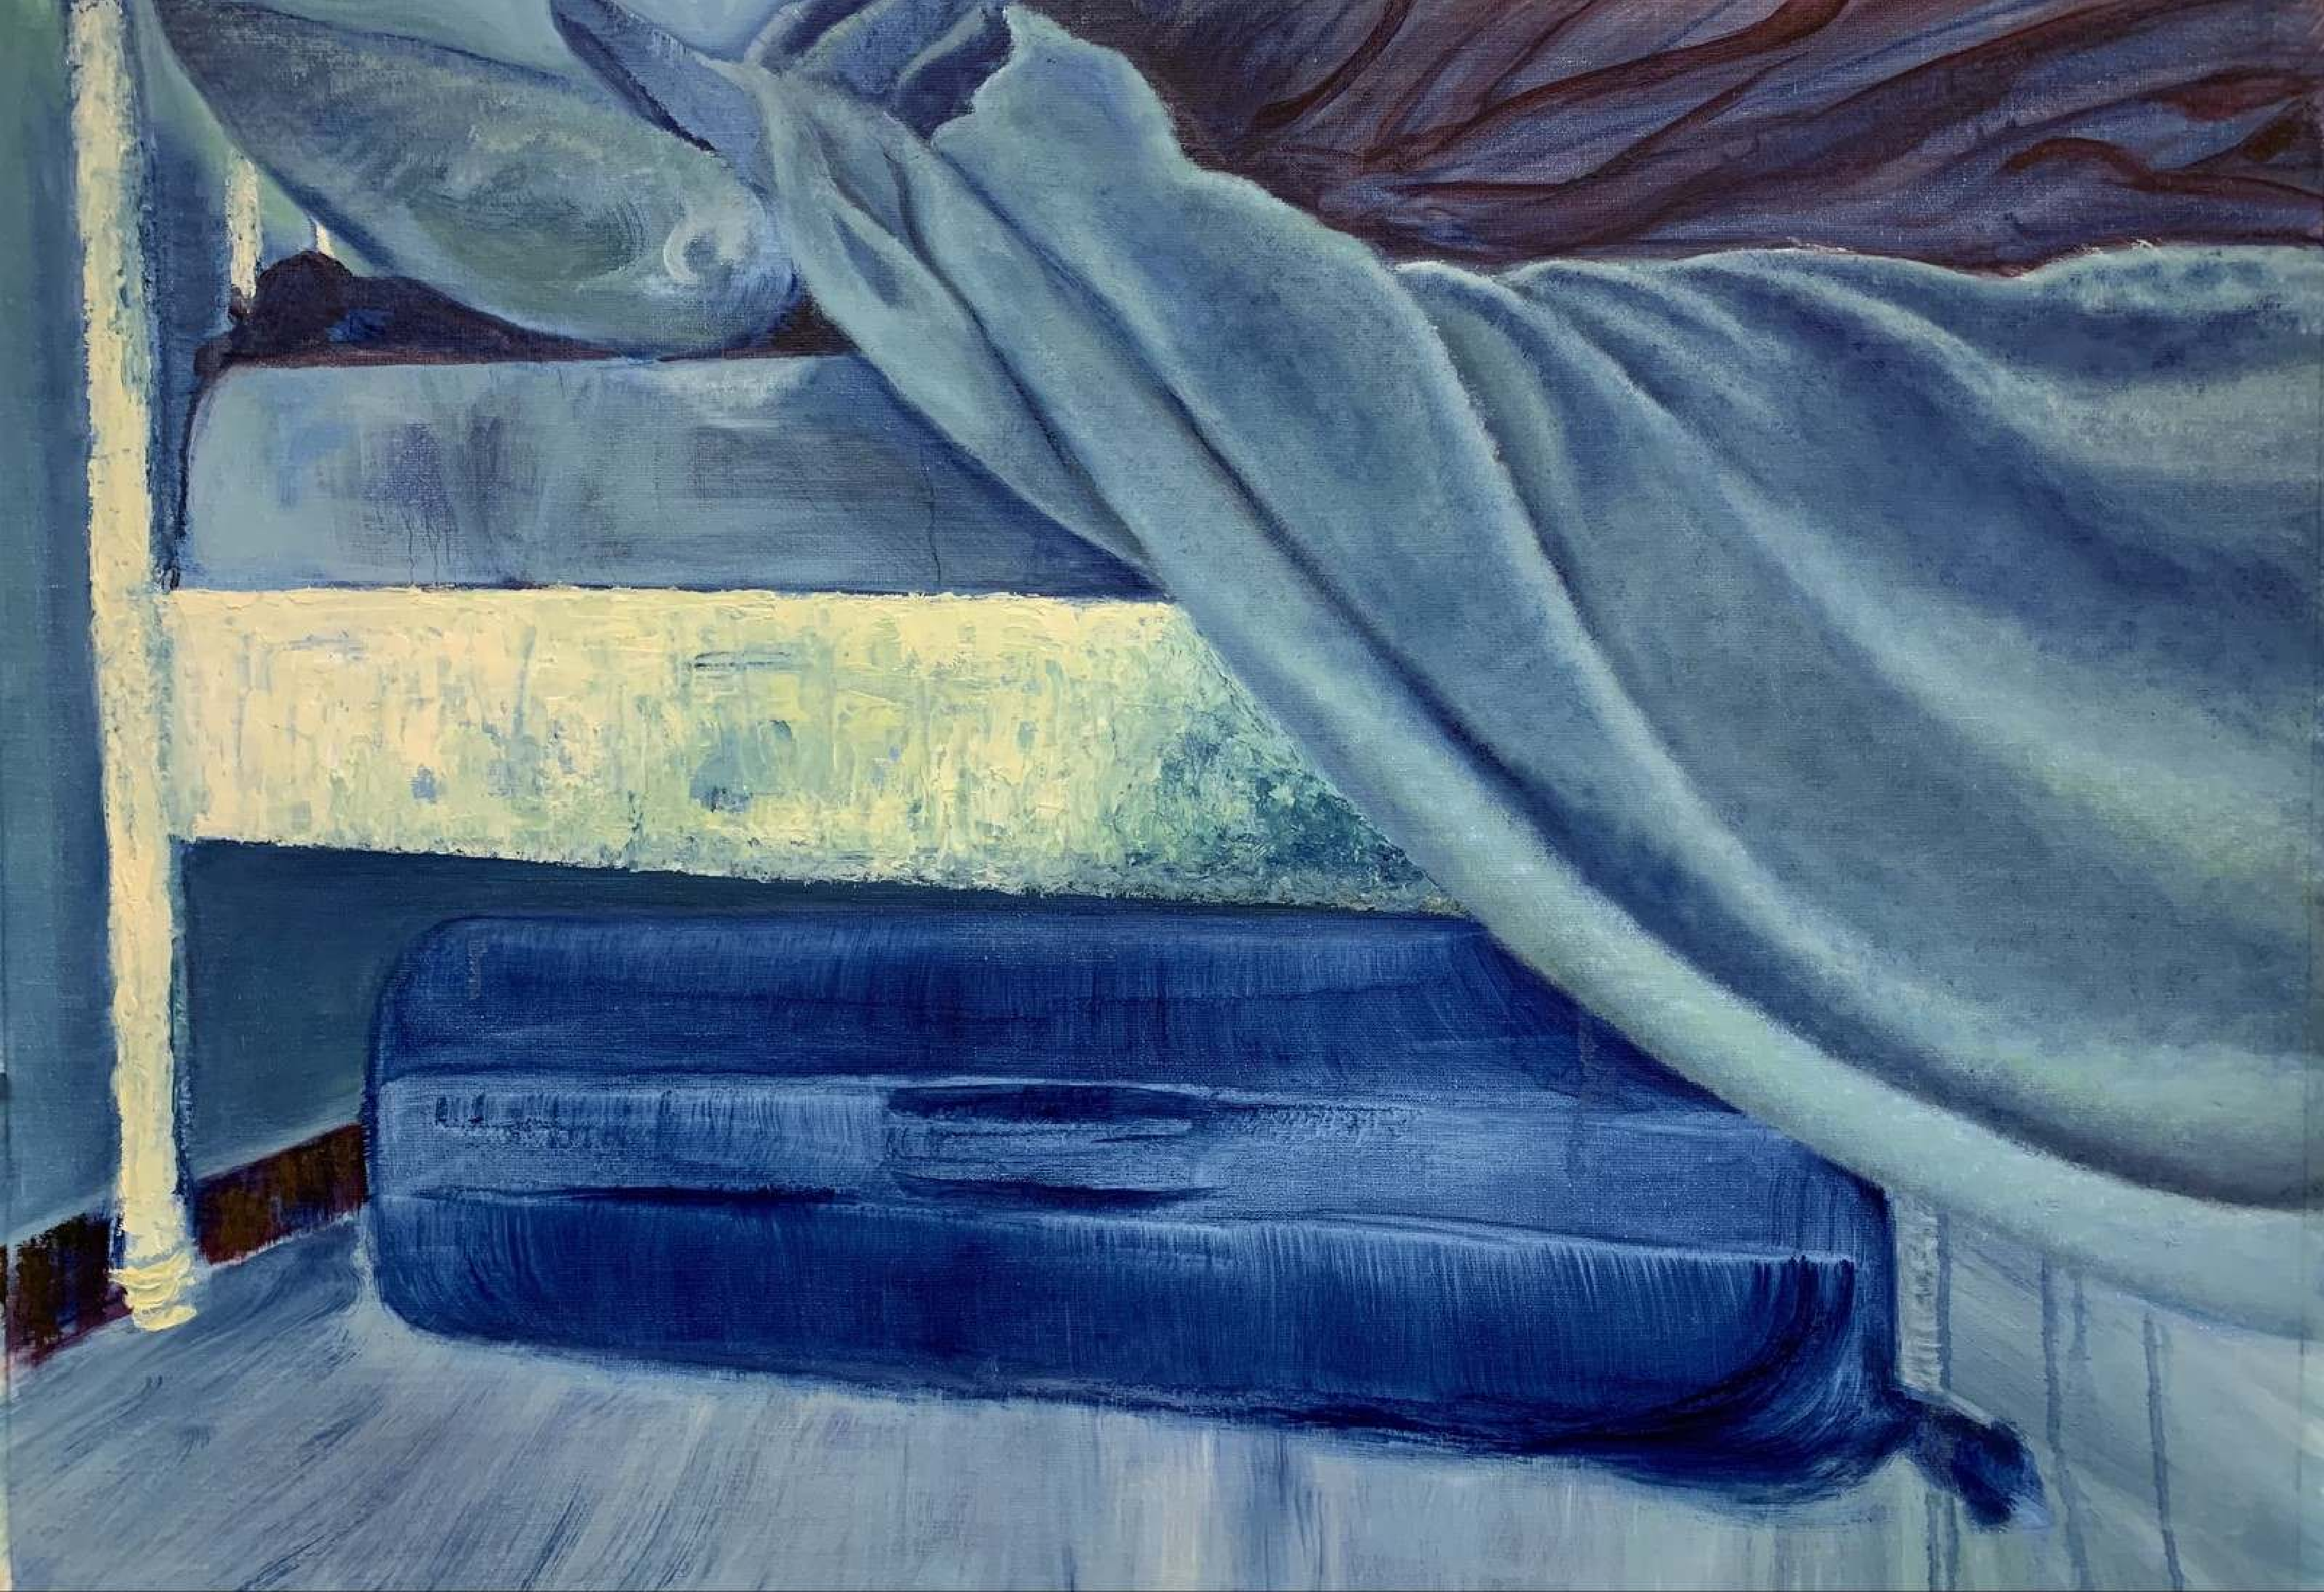
\includegraphics[width = \linewidth]{figuras/boudet-under-the-bed-2021.pdf.compressed.pdf}
	\figurenote{\series{Movimento de câmera}. \oleolinho. \artsize{57.5x82x4}. \\ Foto da autora.}
\end{minipage}\hfill
\begin{minipage}[b]{.25\linewidth}
  \caption{\artname{\odette}{Retrato na parede}{2021}}\label{retrato-na-parede}

	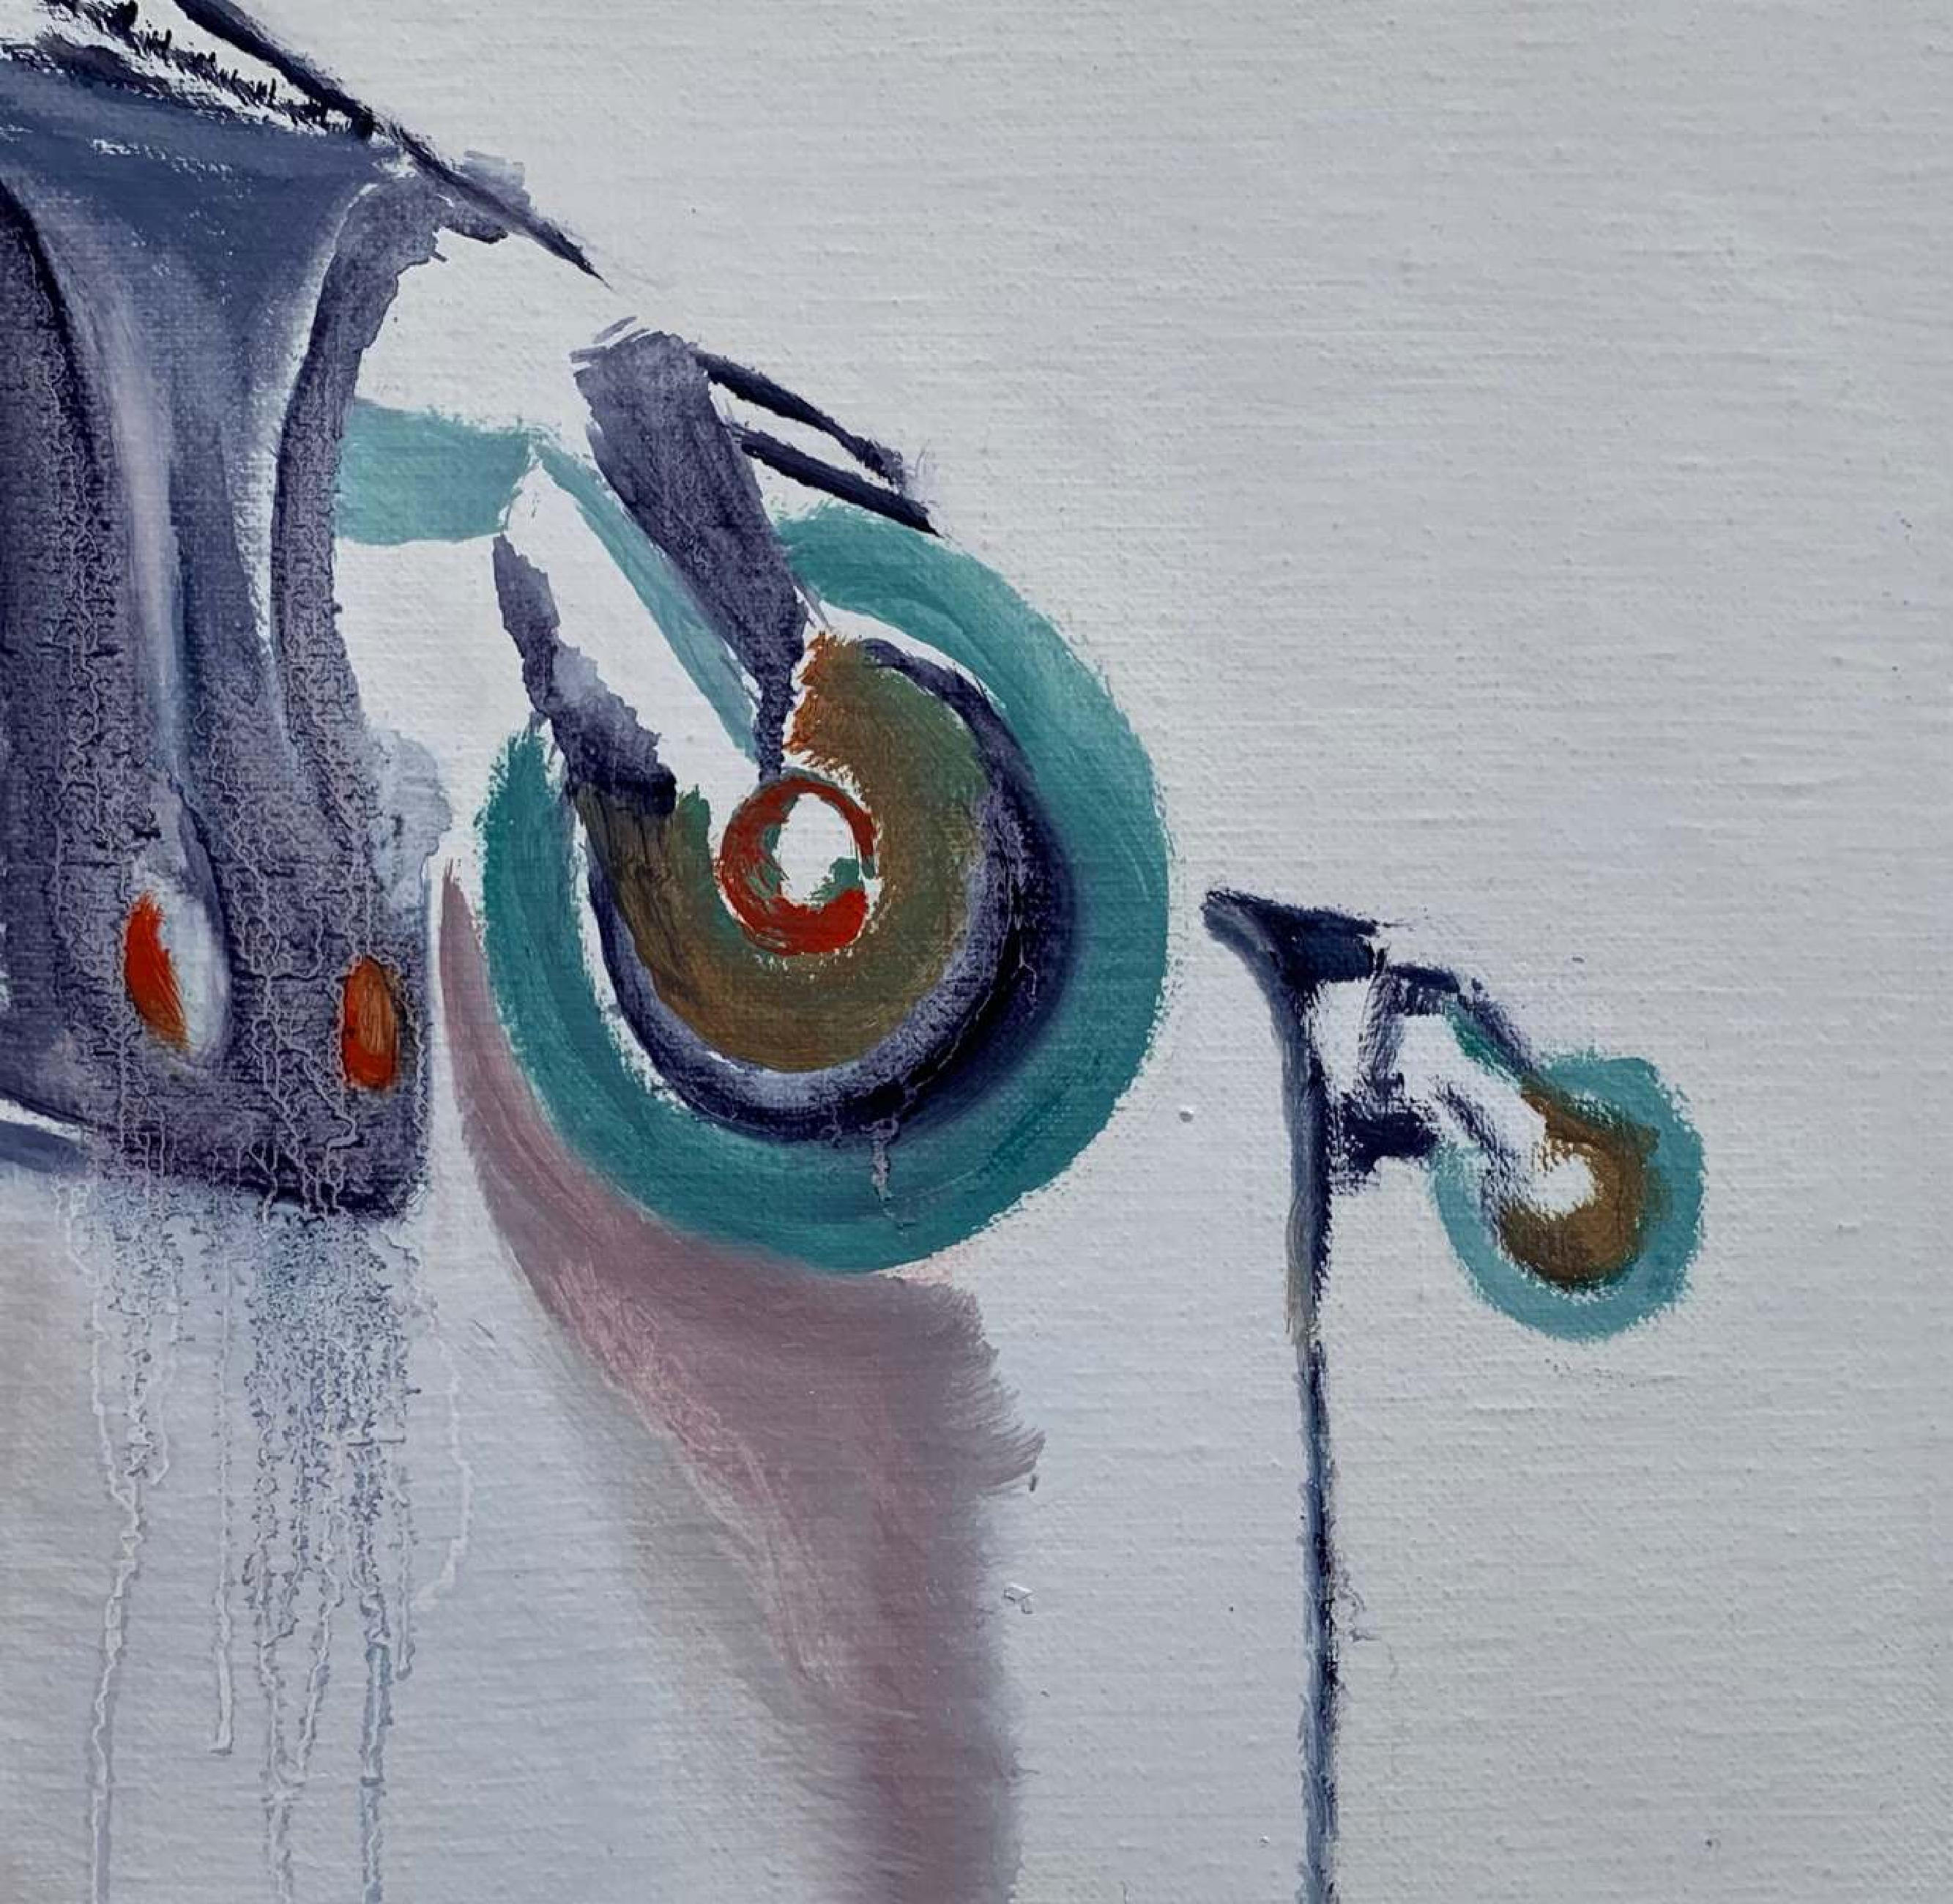
\includegraphics[width=.6\linewidth]{figuras/boudet-retrat-na-parede-2021.pdf.compressed.pdf}
	\figurenote{\series{Movimento de câmera}. \oleolinho. \artsize{20x20x4}. \\ Foto da autora}
\end{minipage}
\end{figure}

\section{Definindo o tema}\label{definindo-o-tema}

Coletar imagens que nos sensibilizam, de forma aleatória pode ajudar a
quem não tem certezas sobre o assunto que quer tratar. A criação de um
banco de imagens e recolha constante de fontes, pode ser um hábito no
processo criativo de um pintor, que o ajudará muitas vezes a escolher o
quê, o porquê e o como na elaboração de um projeto artístico. A partir
desta coleta inicial, é possível identificar os conceitos de maior
interesse através de sua recorrência.

No processo de criação do projeto \emph{Olhar do Cinema}, observei a
minha produção de pintura desde o seu início, passando pelas decisões
de trabalhar com pintura a óleo e figurativa, até chegar ao ponto em
que me encontro, visando a execução de um projeto que se relacione com
o tema desta dissertação. A produção de pintura já tinha uma longa
estrada e são muitas as imagens que carrego nas costas. O \emph{Atlas
	Mnemosyne} de Aby Warburg me inspirava e a Mala que Walter Benjamin
deixou com seus escritos inacabados, também. Como organizar e
selecionar tantas informações e interesses? Optei por separar as
referências em pastas no aplicativo Pinterest (\cref{o-esbouxe7o-o-quadro-o-formato-e-o-projetor})
, visando escolher um
ponto de partida. A motivação inicial de querer saber como se constrói
uma imagem através do olhar do cinema deu nome às pastas:
\emph{movimento, olhar, humano e cenário.}

\begin{figure}
	\caption{Capturas de ecrã. }

	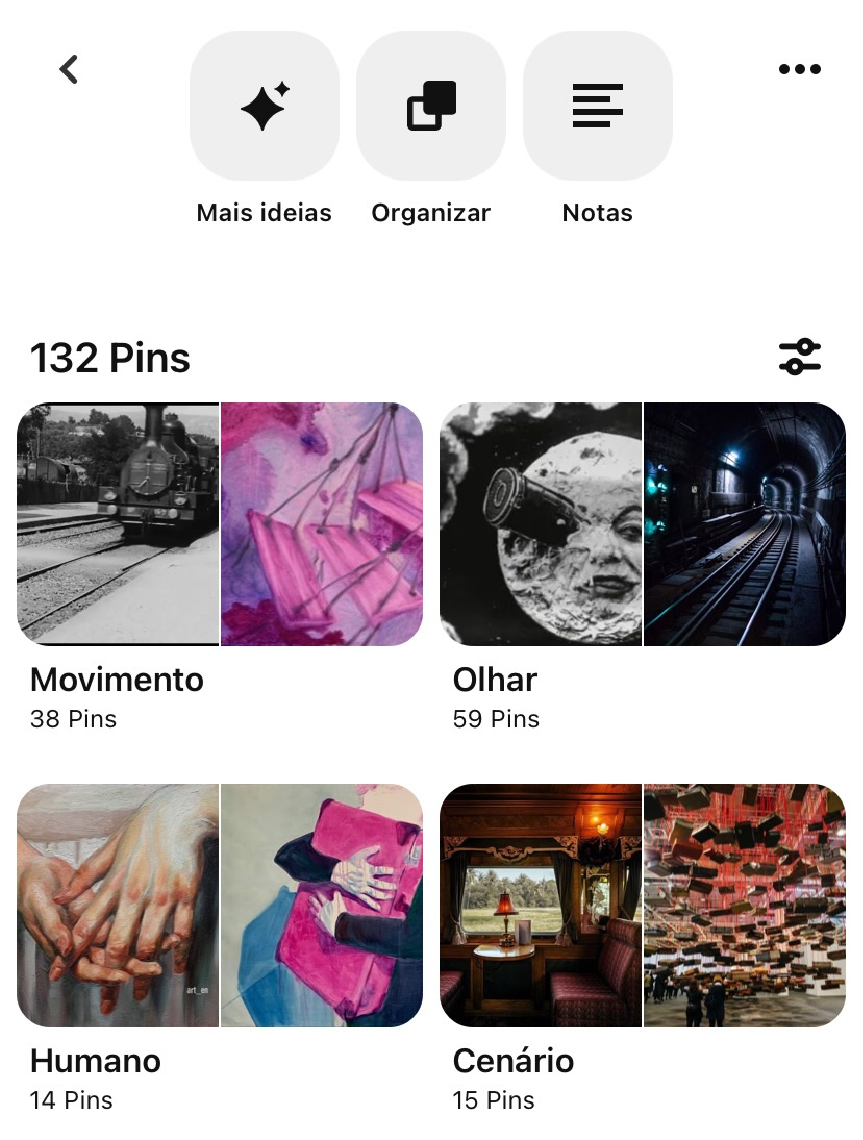
\includegraphics[width=2.33526in,height=3.08547in]{figuras/captura-ecra.pdf.compressed.pdf}
	\figurenote{Fonte: página do Pinterest da autora}
\end{figure}

\section{O esboço, o quadro, o formato e o projetor}%
\label{o-esbouxe7o-o-quadro-o-formato-e-o-projetor}

\paragraph{O esboço} Após definir os primeiros temas, o segundo passo para a criação do
projeto seria a realização de esboços, um hábito que eu não tinha, pois
sempre parti diretamente para a realização do trabalho final. Para esta
etapa seria necessário selecionar referências e decidir o formato que
iria trabalhar: a janela e o quadro, onde tudo começa.

\paragraph{O quadro} Levando em conta estes aspectos abordados no \cref{cap1-contexto-relacao-cinema-pintura}, ao tratar das
teorias relacionadas a espaço, concluímos que um dos pontos de
interseção mais claros entre o cinema e a pintura certamente é o
\emph{quadro}. As relações com o quadro, seus limites e o desejo de
transformá-lo em uma janela para o mundo real é objeto do texto de
Jacques Aumont sobre o quarto de Van Gogh. Esta janela hoje tem um
nome: a câmera de um celular e seus muitos aplicativos. Outro exemplo
sobre o quadro é o \emph{assunto} da pintura da Lúcia Laguna, que se
encontra do outro lado da Janela. Hitchcock faz uma verdadeira ode ao
quadro em seu filme \emph{A janela indiscreta (1954)} e Woody Allen
leva seu personagem em \emph{A Rosa púrpura do Cairo (1985)}
literalmente para dentro do espaço narrativo do filme.

\paragraph{O formato} Ao iniciar uma pintura, nos moldes tradicionais sobre um suporte em
tela, painel, é preciso contar com estes limites e decidir o seu
formato. Nosso objetivo de criar um projeto artístico de
pintura sobre tela precisou refletir, logo no início, sobre este
aspecto.

Por muito tempo, no meu caso, esta decisão se relacionava diretamente
com a imagem fotográfica de referência e com a estratégia compositiva
dos seus elementos, que em geral eram posicionados por meio da análise
de \emph{golden lines}.

Como já mencionado no início deste capítulo, sobre a Série
\emph{Penumbra}, o meu processo se iniciava com um ensaio de
fotografias que eram projetadas sobre a tela ou linho grampeados na
parede, com a finalidade de realizar o esboço através de pintura
indireta. As reflexões sobre a composição da imagem começam, já nos
recortes da fotografia que será projetada. Este é um processo que uso
há muitos anos e as decisões finais sobre o formato em geral ocorrem
neste momento inicial de projeção.

A pandemia direcionou nossas exposições para o espaço virtual. Em
consequência, optei por unificar o formato de todas as obras para o
quadrado. Dois motivos me levaram a esta decisão: a ideia da formação
da imagem audiovisual em pixels; e os formatos de aplicativos nas redes
de compartilhamento como Instagram, para ecrãs dos celulares\slash
telemóveis.

\paragraph{O projetor} Com o formato definido, é preciso ainda checar se o arquivo da imagem
tem a sua extensão apropriada para uso no projetor, que de preferência
deve ter mais de 3000 lumens. Neste momento começa a melhor parte.
Nosso corpo se interpõe entre a luz do projetor e a tela que será
abordada por instrumentos da pintura. A experiência de estar em uma
sala de cinema é trazida de volta e neste momento, é possível abandonar
um pouco a rigidez de todo um planejamento prévio. O mundo do cinema e
o da pintura se encontram de certa forma nesta hora.

A marcação por meio de projetores para iniciar um trabalho pictórico,
método muitas vezes usado por pintores contemporâneos, vem se somar aos
tradicionais esboços com os modelos vivos e técnicas de ampliação de
desenho. Podemos afirmar que esta parte do meu processo criativo
acontece de maneira indireta, onde os modelos do mundo real já sofreram
um tratamento por outros meios de representação da imagem, no caso a
fotografia e o cinema.

\section{O desenvolvimento do projeto}%
\label{o-desenvolvimento-do-projeto}

Retomando a questão do tema, elaborei alguns esboços em ateliê para
representar as imagens coletadas, com ideias de movimento, olhar,
humano e cenário. Ícones dos primeiros filmes: o trem dos irmãos
Lumière e \emph{Viagem à Lua} de Méliès foram as imagens escolhidas
para os primeiros esboços, com a finalidade de \emph{aquecer os
	pincéis} e de realizar testes de cor, moldes, suportes e formatos. Para
estes testes, agreguei referências de processos de alguns pintores como
Gerhard Richter.

\begin{figure}
  \begin{minipage}[t]{.4\linewidth}
    \caption{Esboço Série Olhar do Cinema. Teste Phtalo blue. \phantom{aaaaaaaaaaaaaaaaaaaaaaaaaaaa}}
	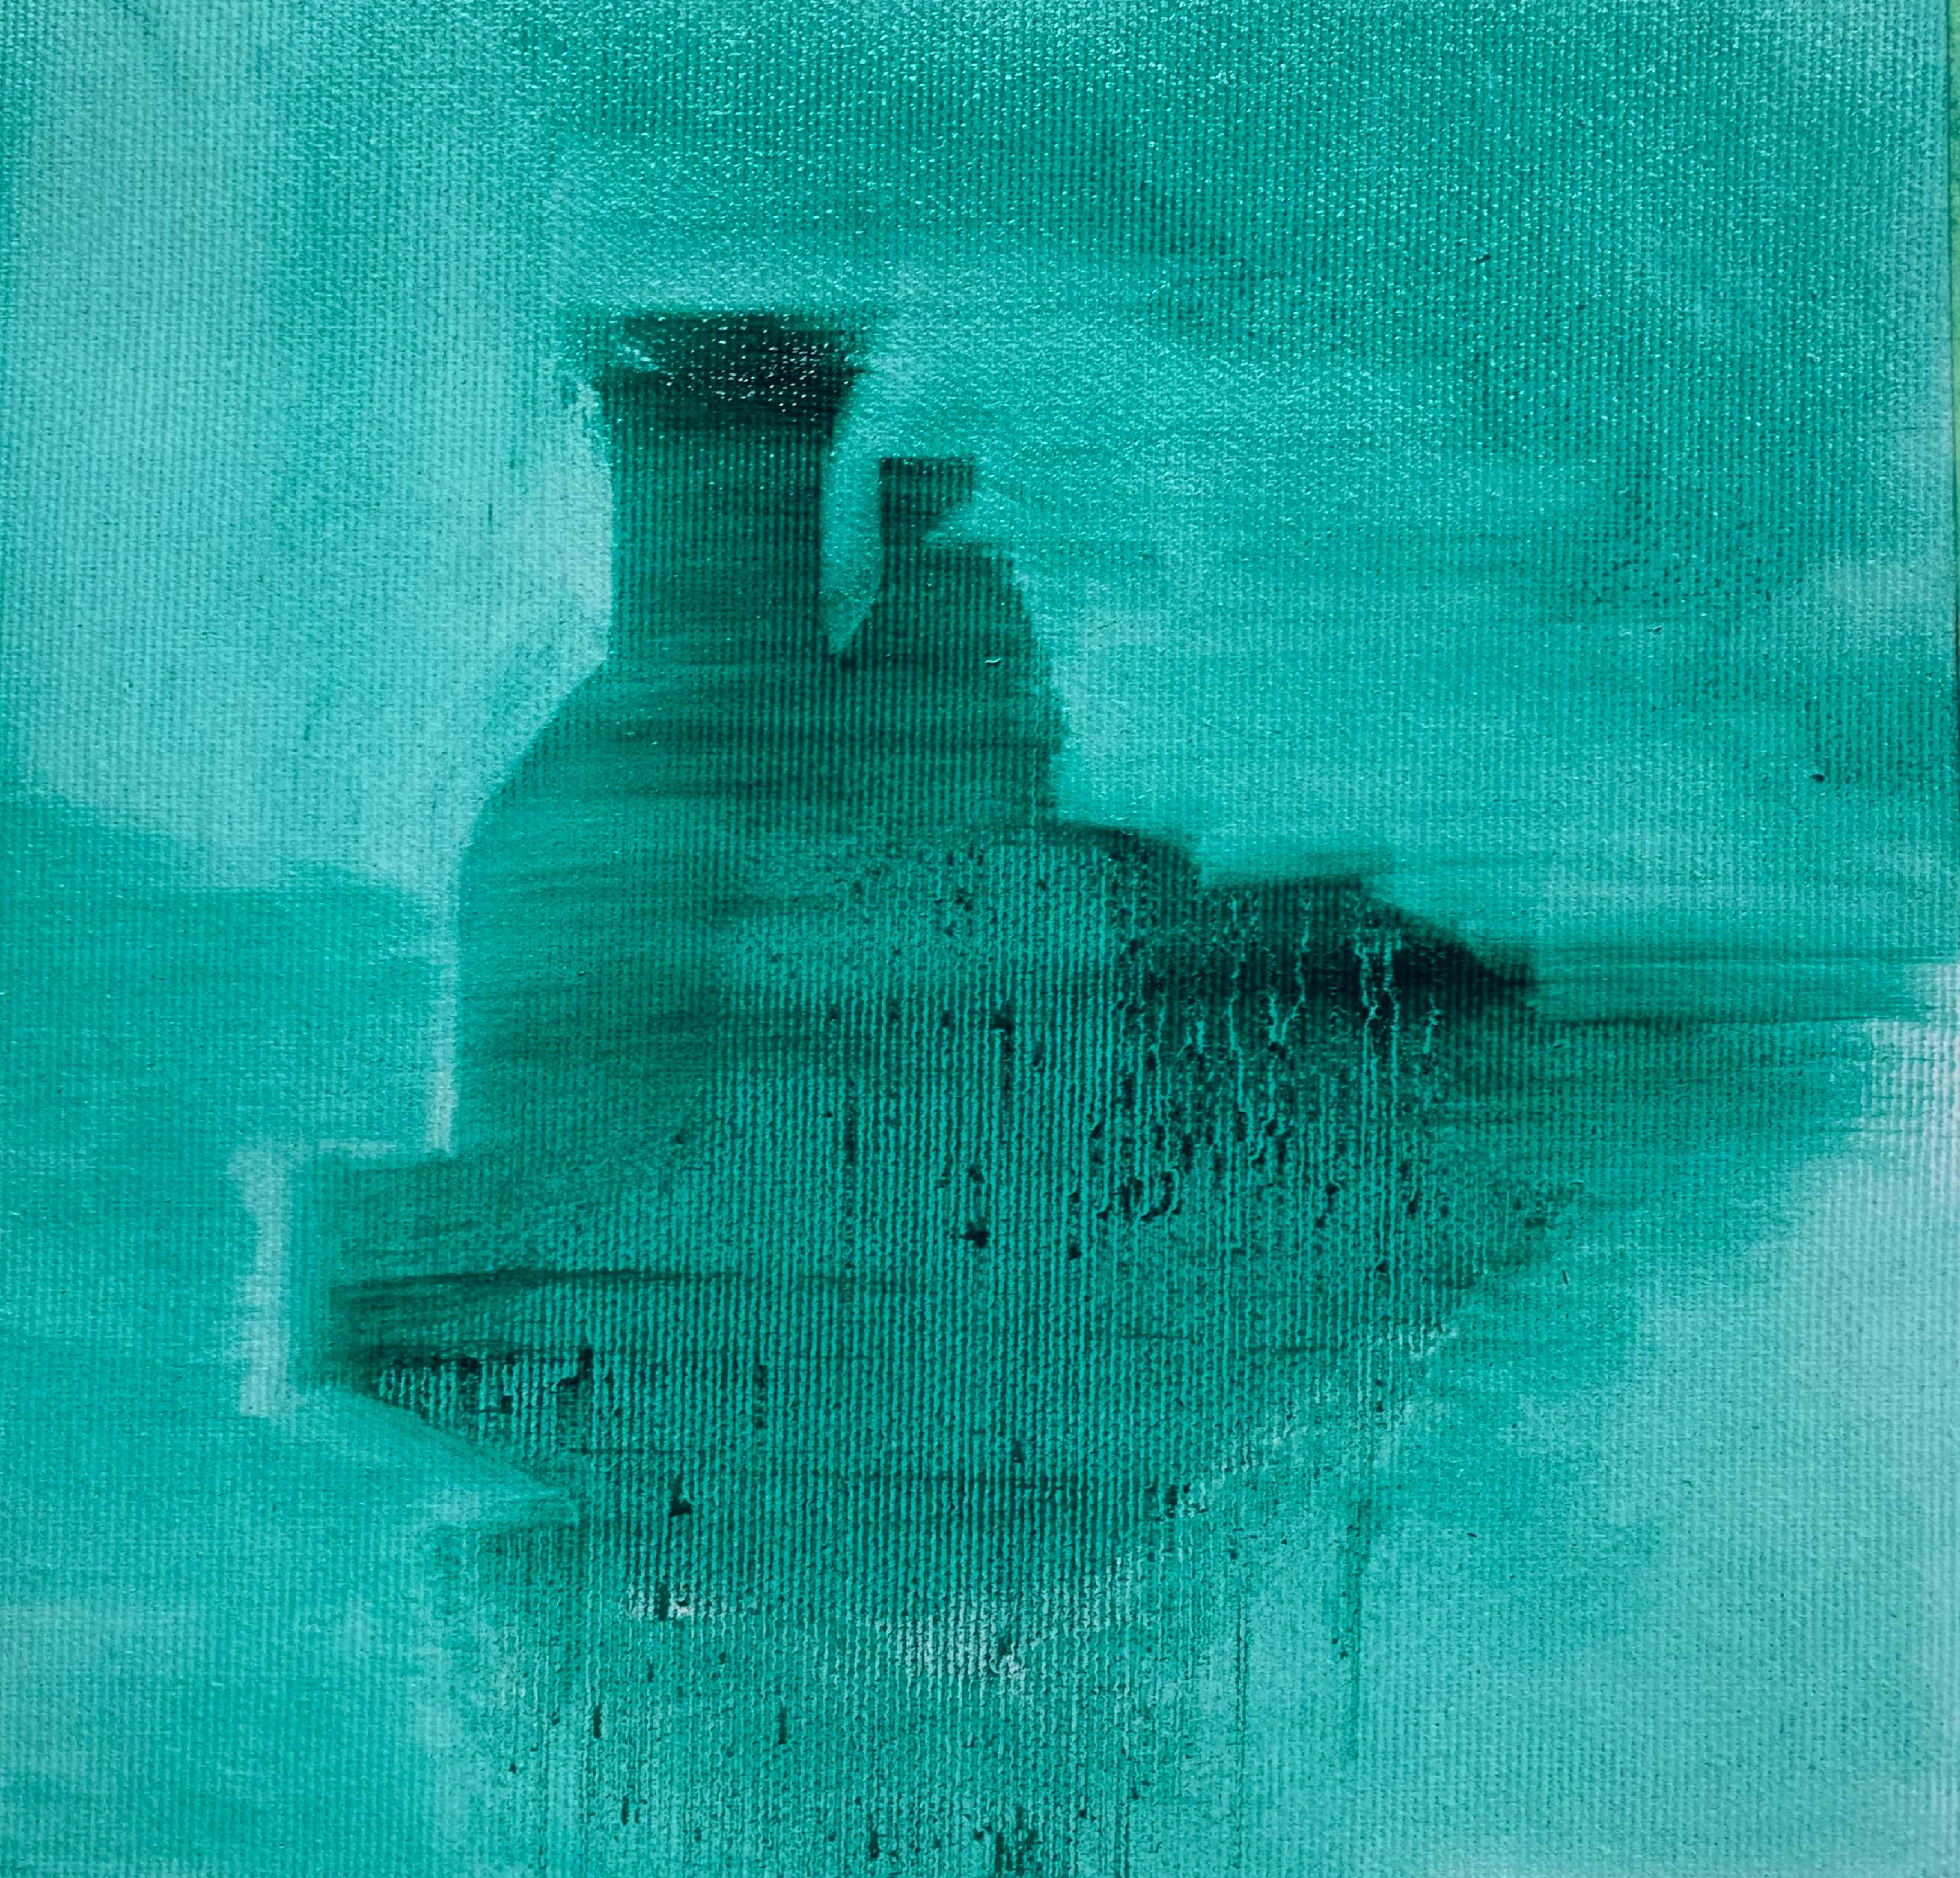
\includegraphics[height=1.30866in]{figuras/boudet-esboco-olhar-do-cinema.pdf.compressed.pdf}
	\figurenote{Artista de referência Gerhard Richter. \oleo. \artsize{20x20}. Foto da autora.}
\end{minipage}\hfill
\begin{minipage}[t]{.4\linewidth}
	\caption{Teste de preto Cromático
		Phtalo Blue e Quinacridona Rose --- \artname{\odette}{Estação Lumière I}{2022}.}

	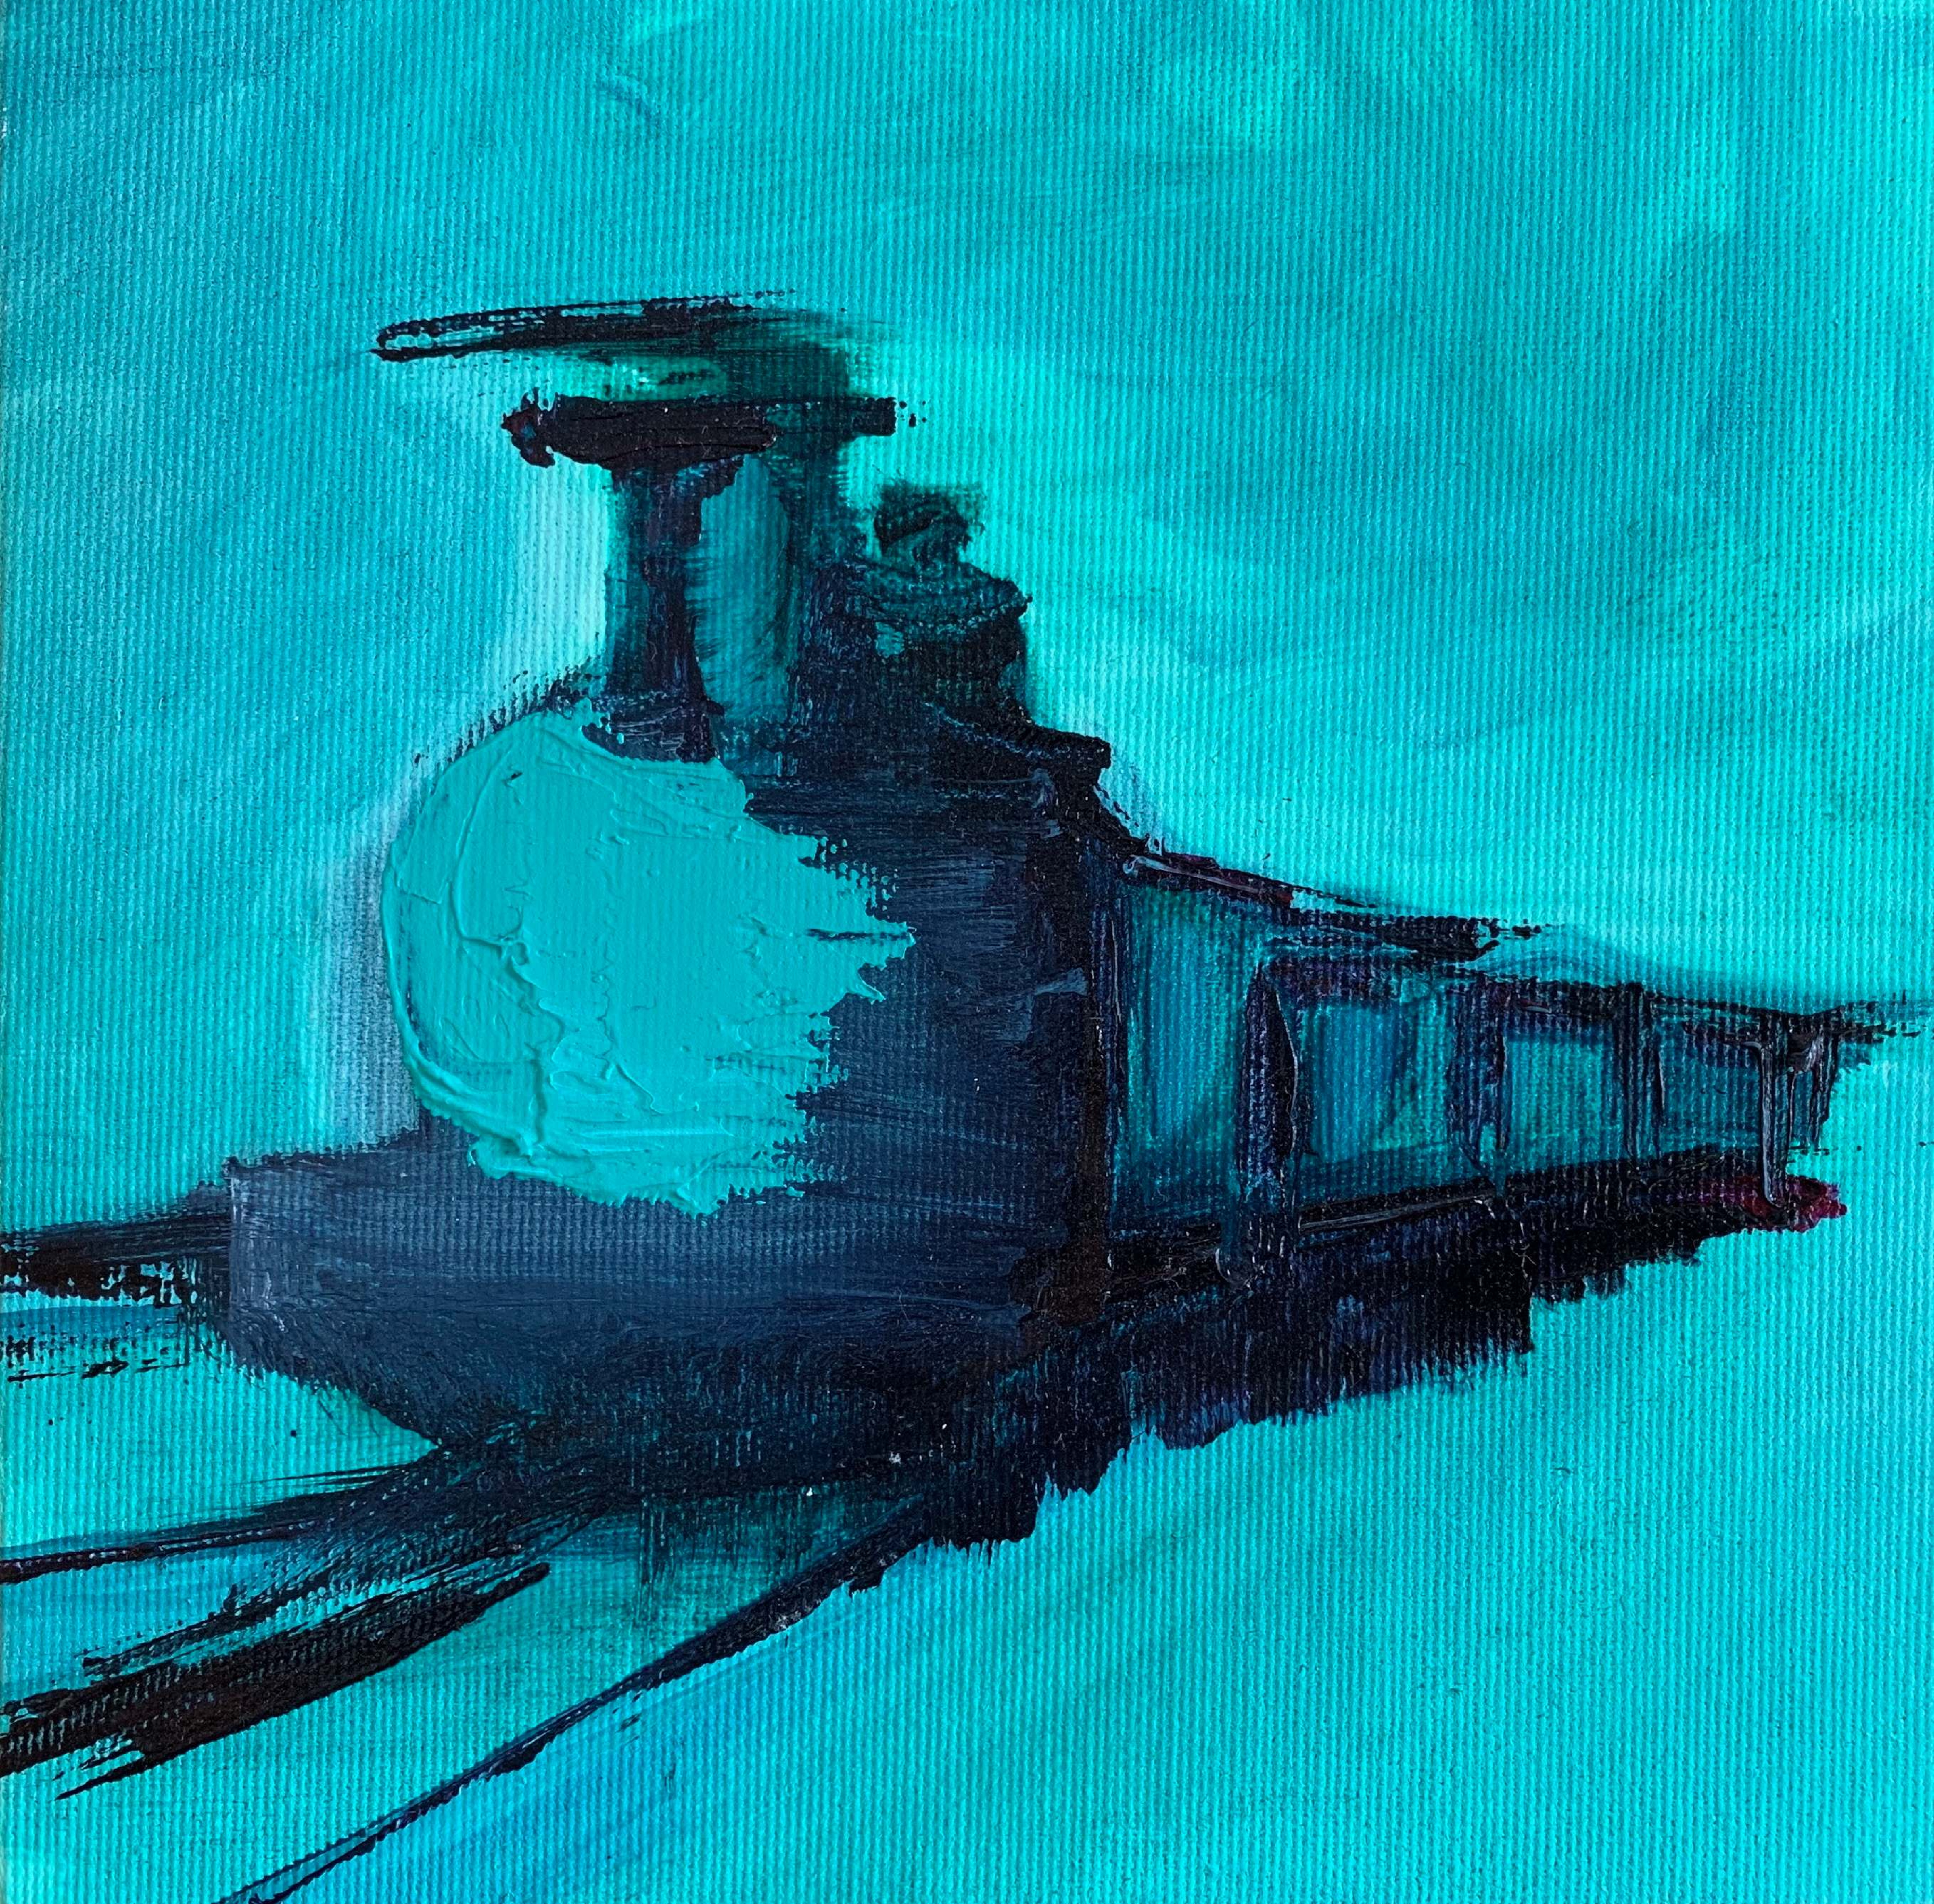
\includegraphics[height=1.30866in]{figuras/boudet-test-preto-cromatico-2022.pdf.compressed.pdf}
  \figurenote{\series{Espaço no ecrã} \oleo. \artsize{20 x 20}. Foto da autora \phantom{aaaaaaaaaaaaaaaaaaa}}
\end{minipage}
\end{figure}

Alguns destes esboços se transformavam em trabalhos finalizados.

\begin{figure}
  \begin{minipage}[t]{.3\linewidth}
	\caption{Molde de máscara vazada em acetato}

	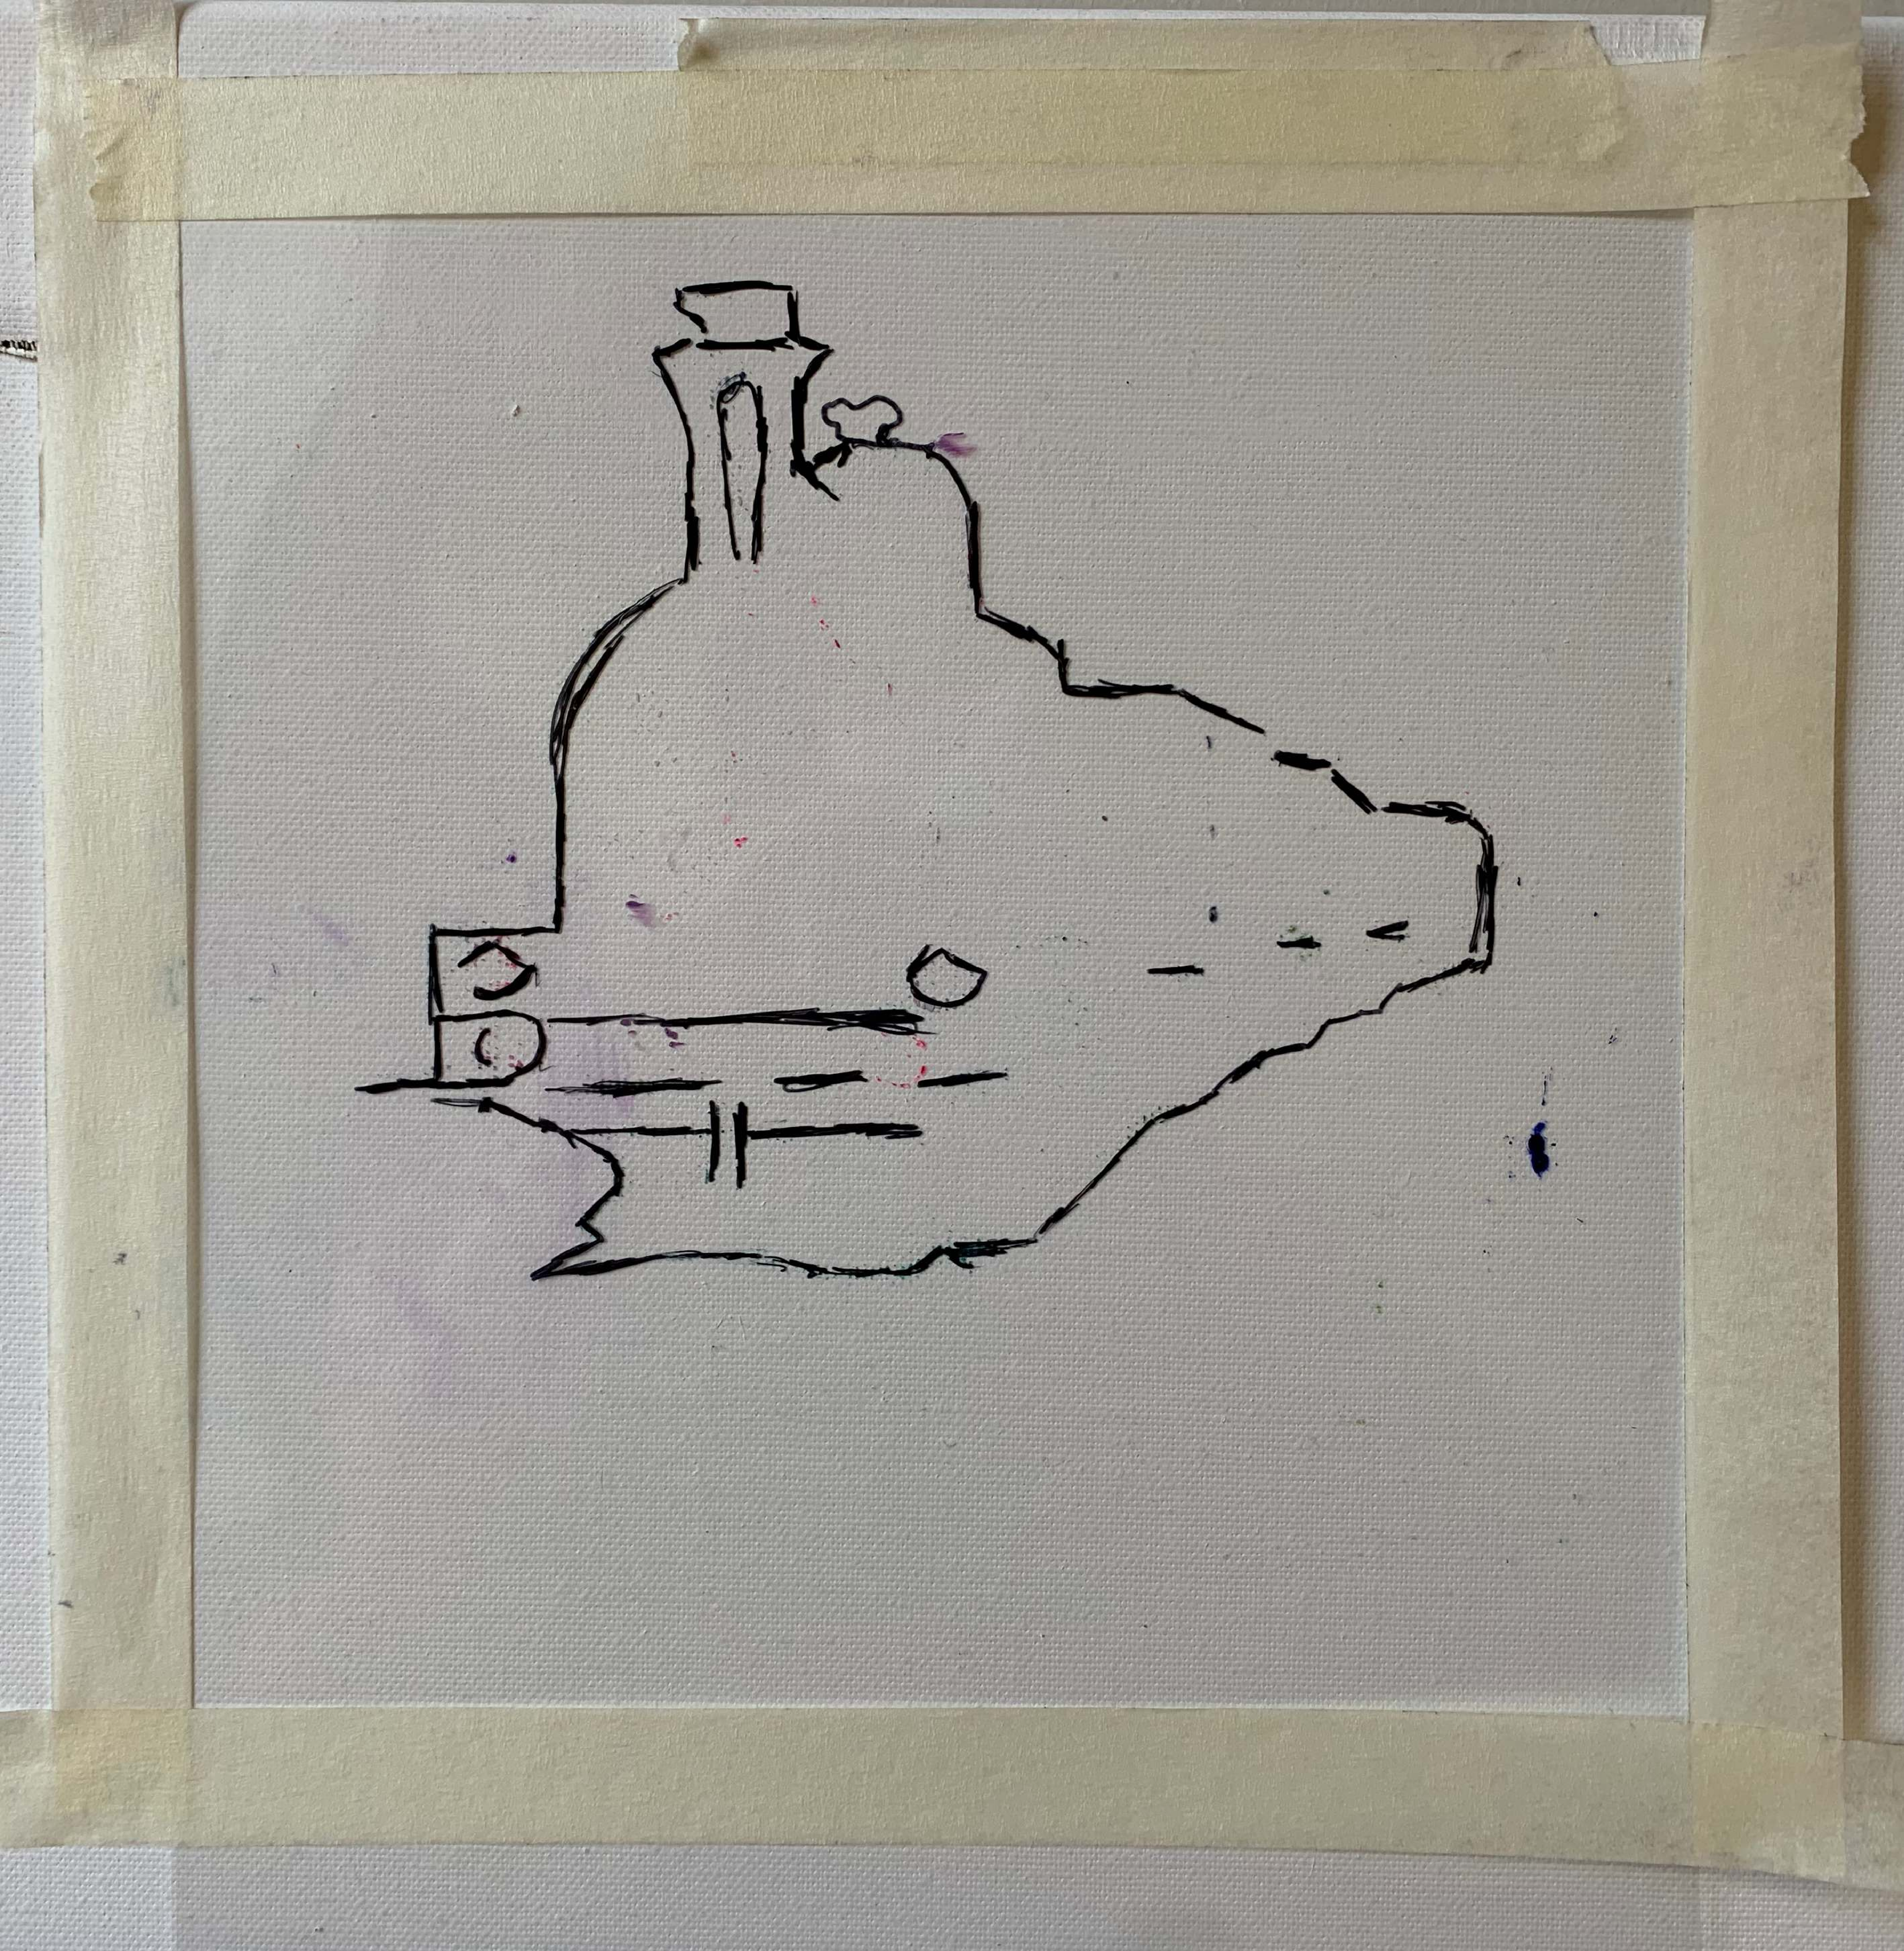
\includegraphics[height=1.30833in]{figuras/molde-mascara-vazada-acetato.pdf.compressed.pdf}
\end{minipage}
\begin{minipage}[t]{.3\linewidth}
	\caption{Esboço fluido do trem sobre molde blocado.}

	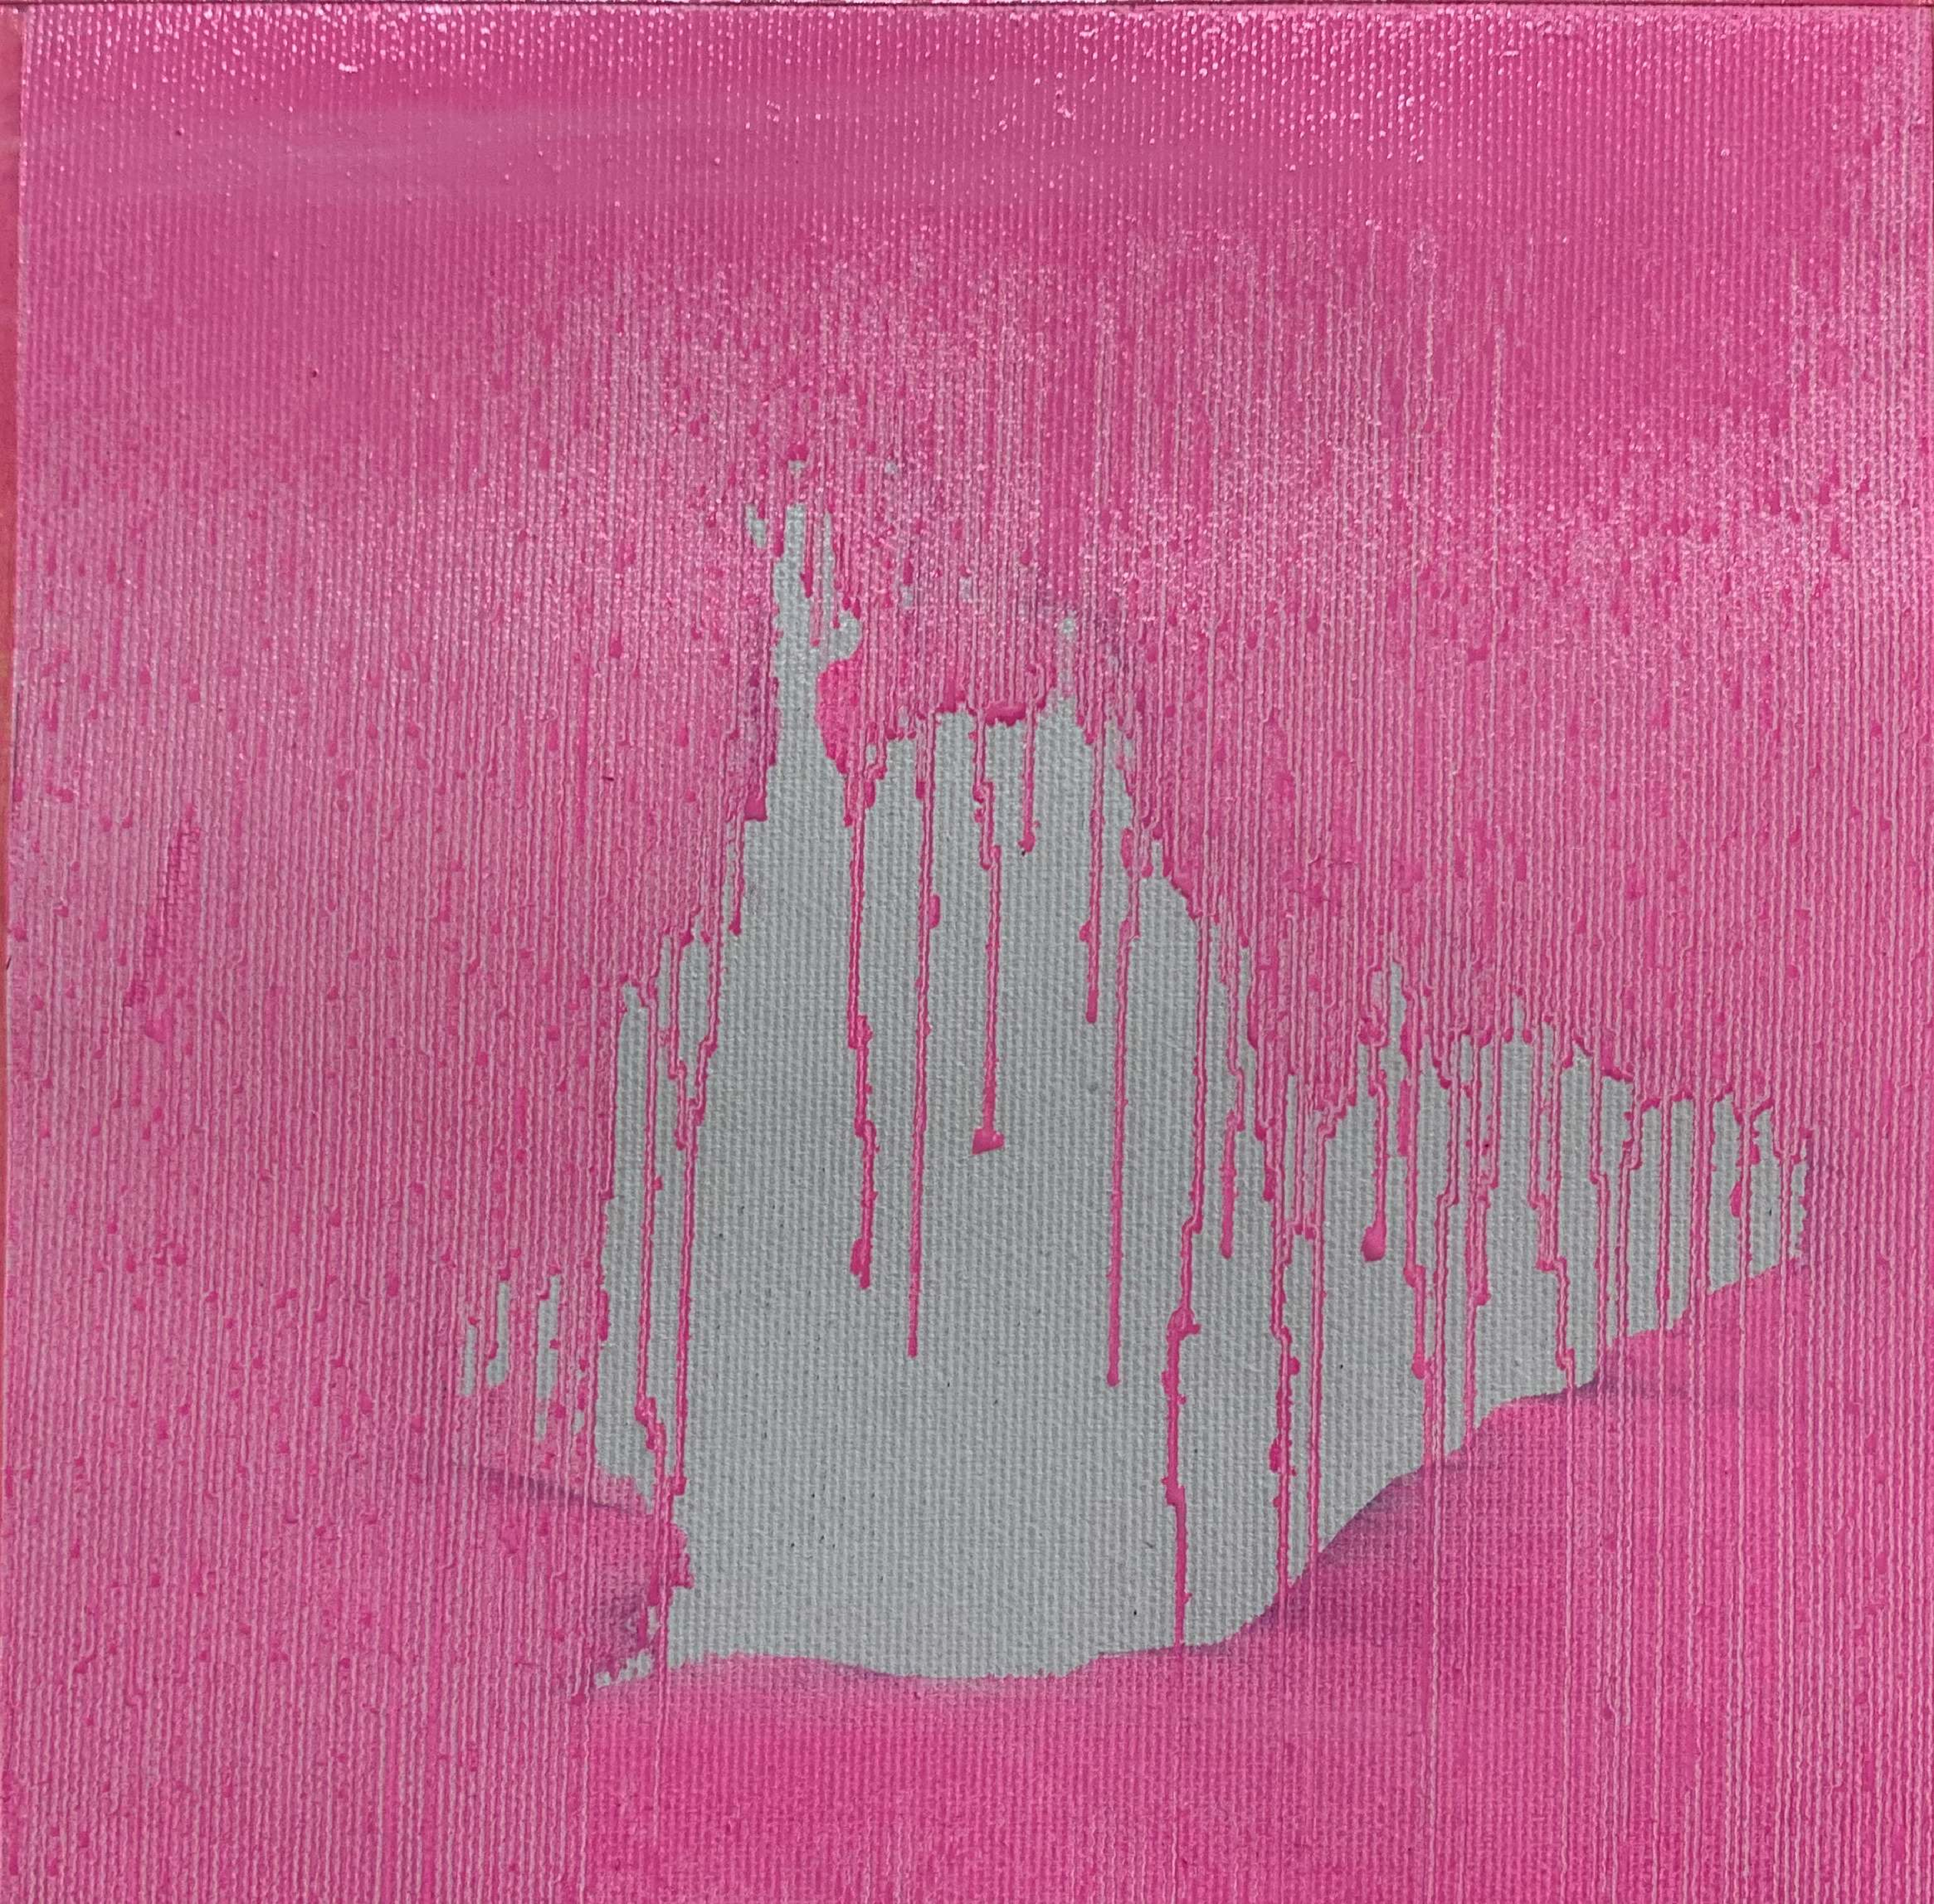
\includegraphics[height=1.30833in]{figuras/esboco-fluido-trem-sobre-molde-blocado.pdf.compressed.pdf}
  \figurenote{Proporção \emph{medium} 1 linhaça para 5 de \emph{white spirit}}
\end{minipage}
  \begin{minipage}[t]{.3\linewidth}
	\caption{Esboço de \enquote{\emph{blurrr}} em máscara vazada.}

	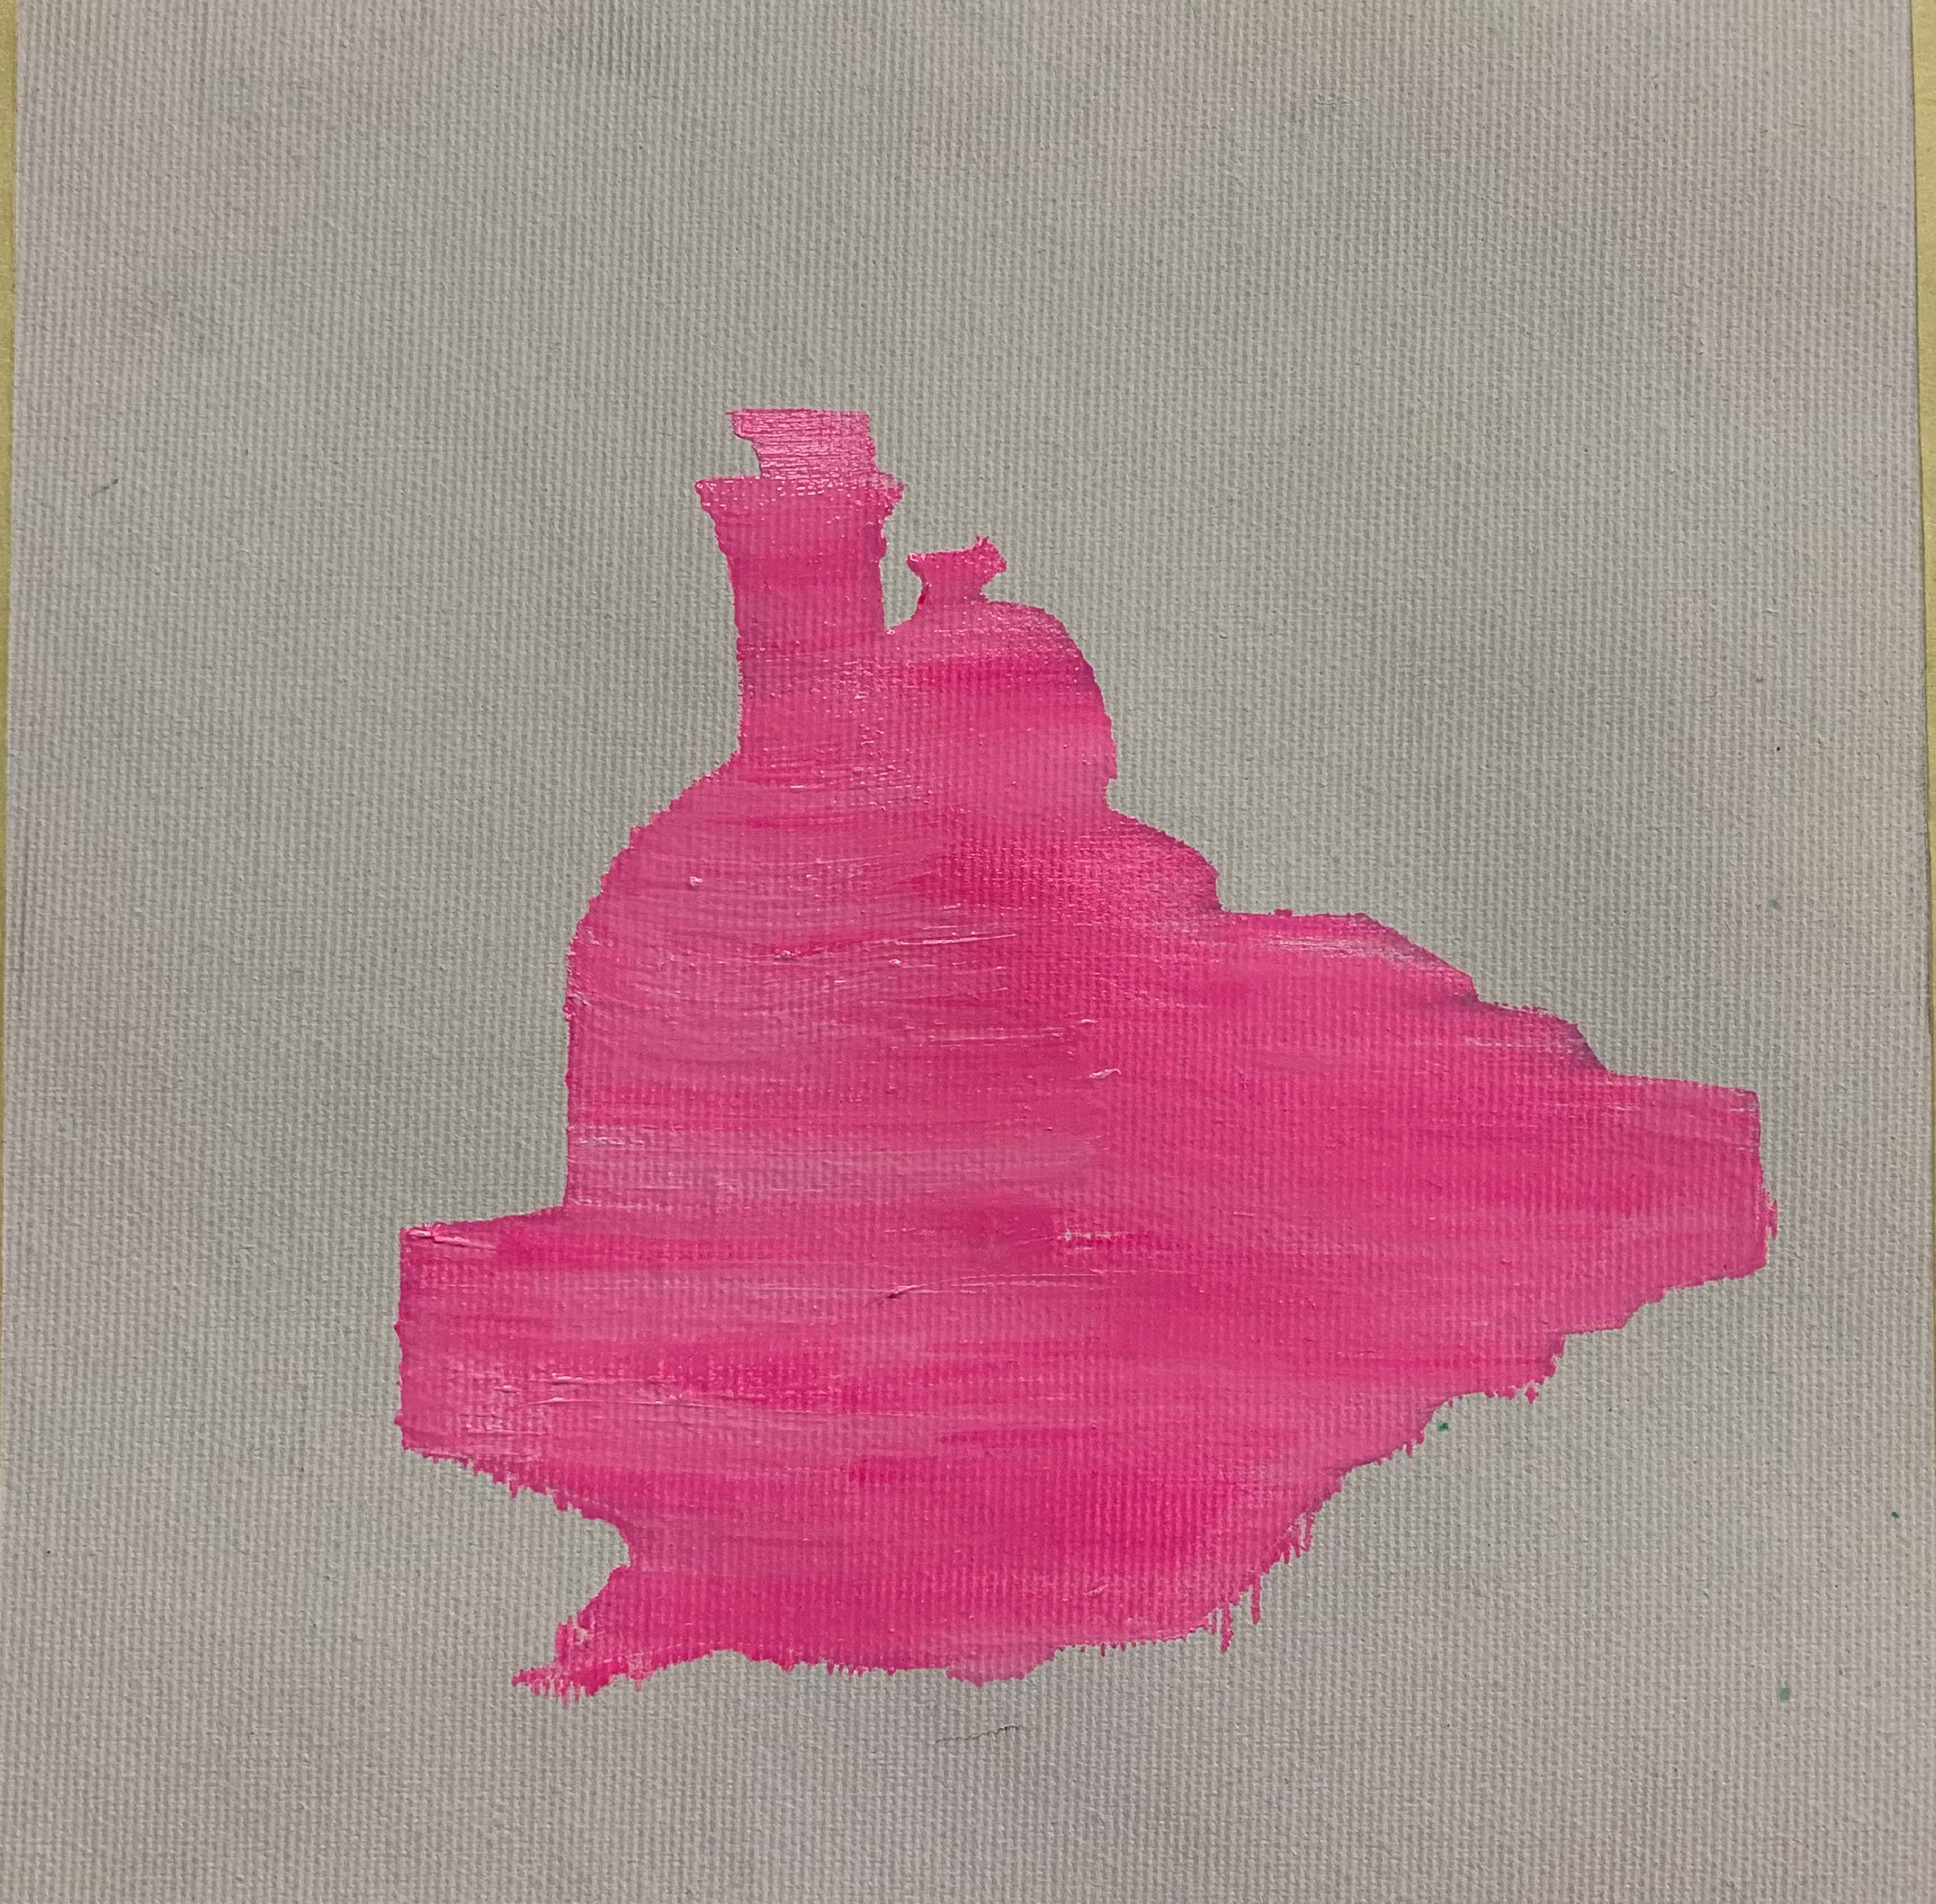
\includegraphics[height=1.30831in]{figuras/esboco-blurrr.pdf.compressed.pdf}
\end{minipage}
\end{figure}


\begin{figure}
\begin{minipage}{.4\linewidth}
	\caption{Processo de William Kentridge --- 7 fragmentos para Georges
		Meliés.}

	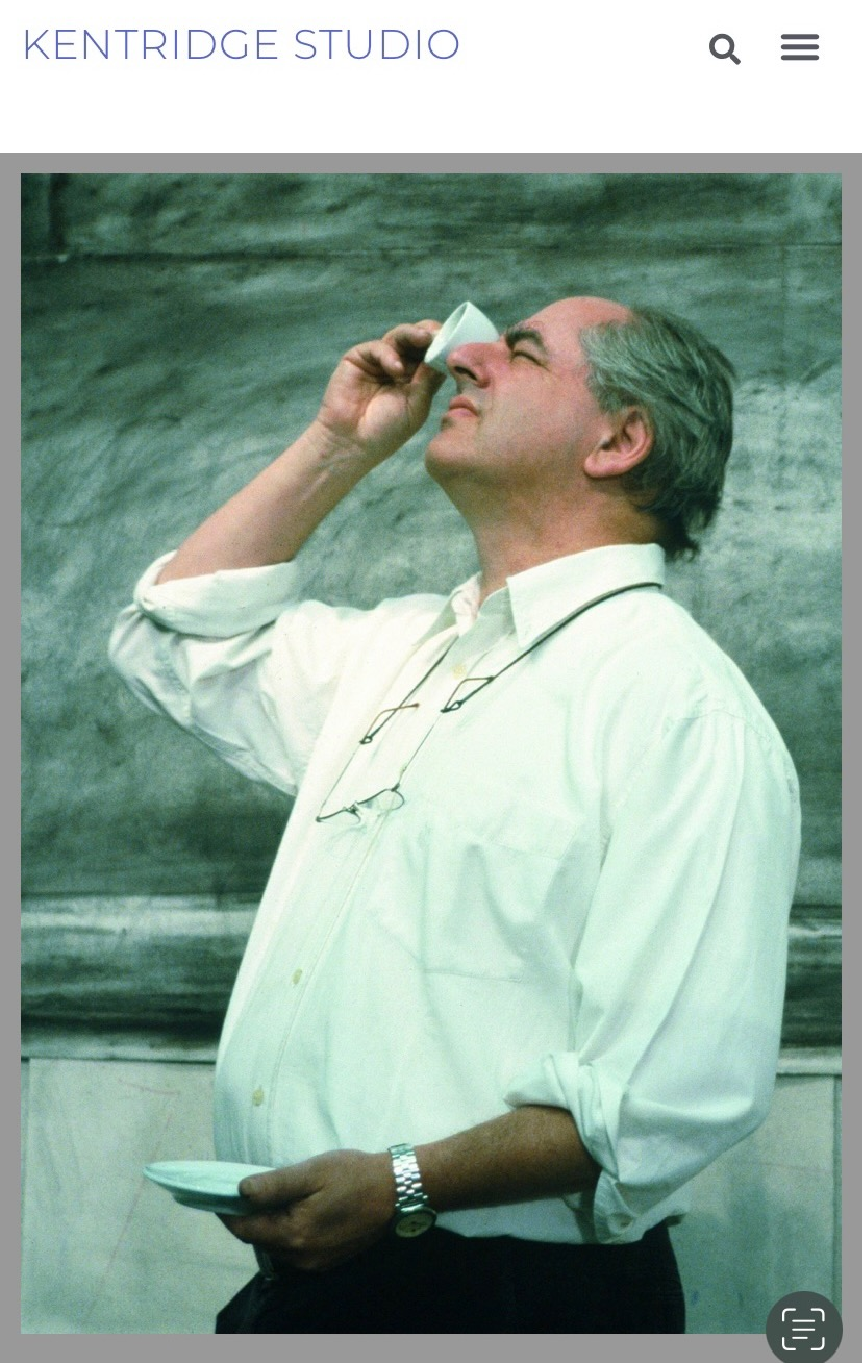
\includegraphics[height=1.98507in]{figuras/kentridge-7-fragmentos-georges-melies.pdf.compressed.pdf}
	\figurenote{Captura de ecrã. Fonte: \hiperlink{http:\\www.kentridge.studio/projects}{Kentridge Studio}}
\end{minipage}\hfill
\begin{minipage}{.4\linewidth}
  \caption{\artname{\odette}{Cena Méliès I}{2022} \phantom{aaaaaaaaaaaa}}

	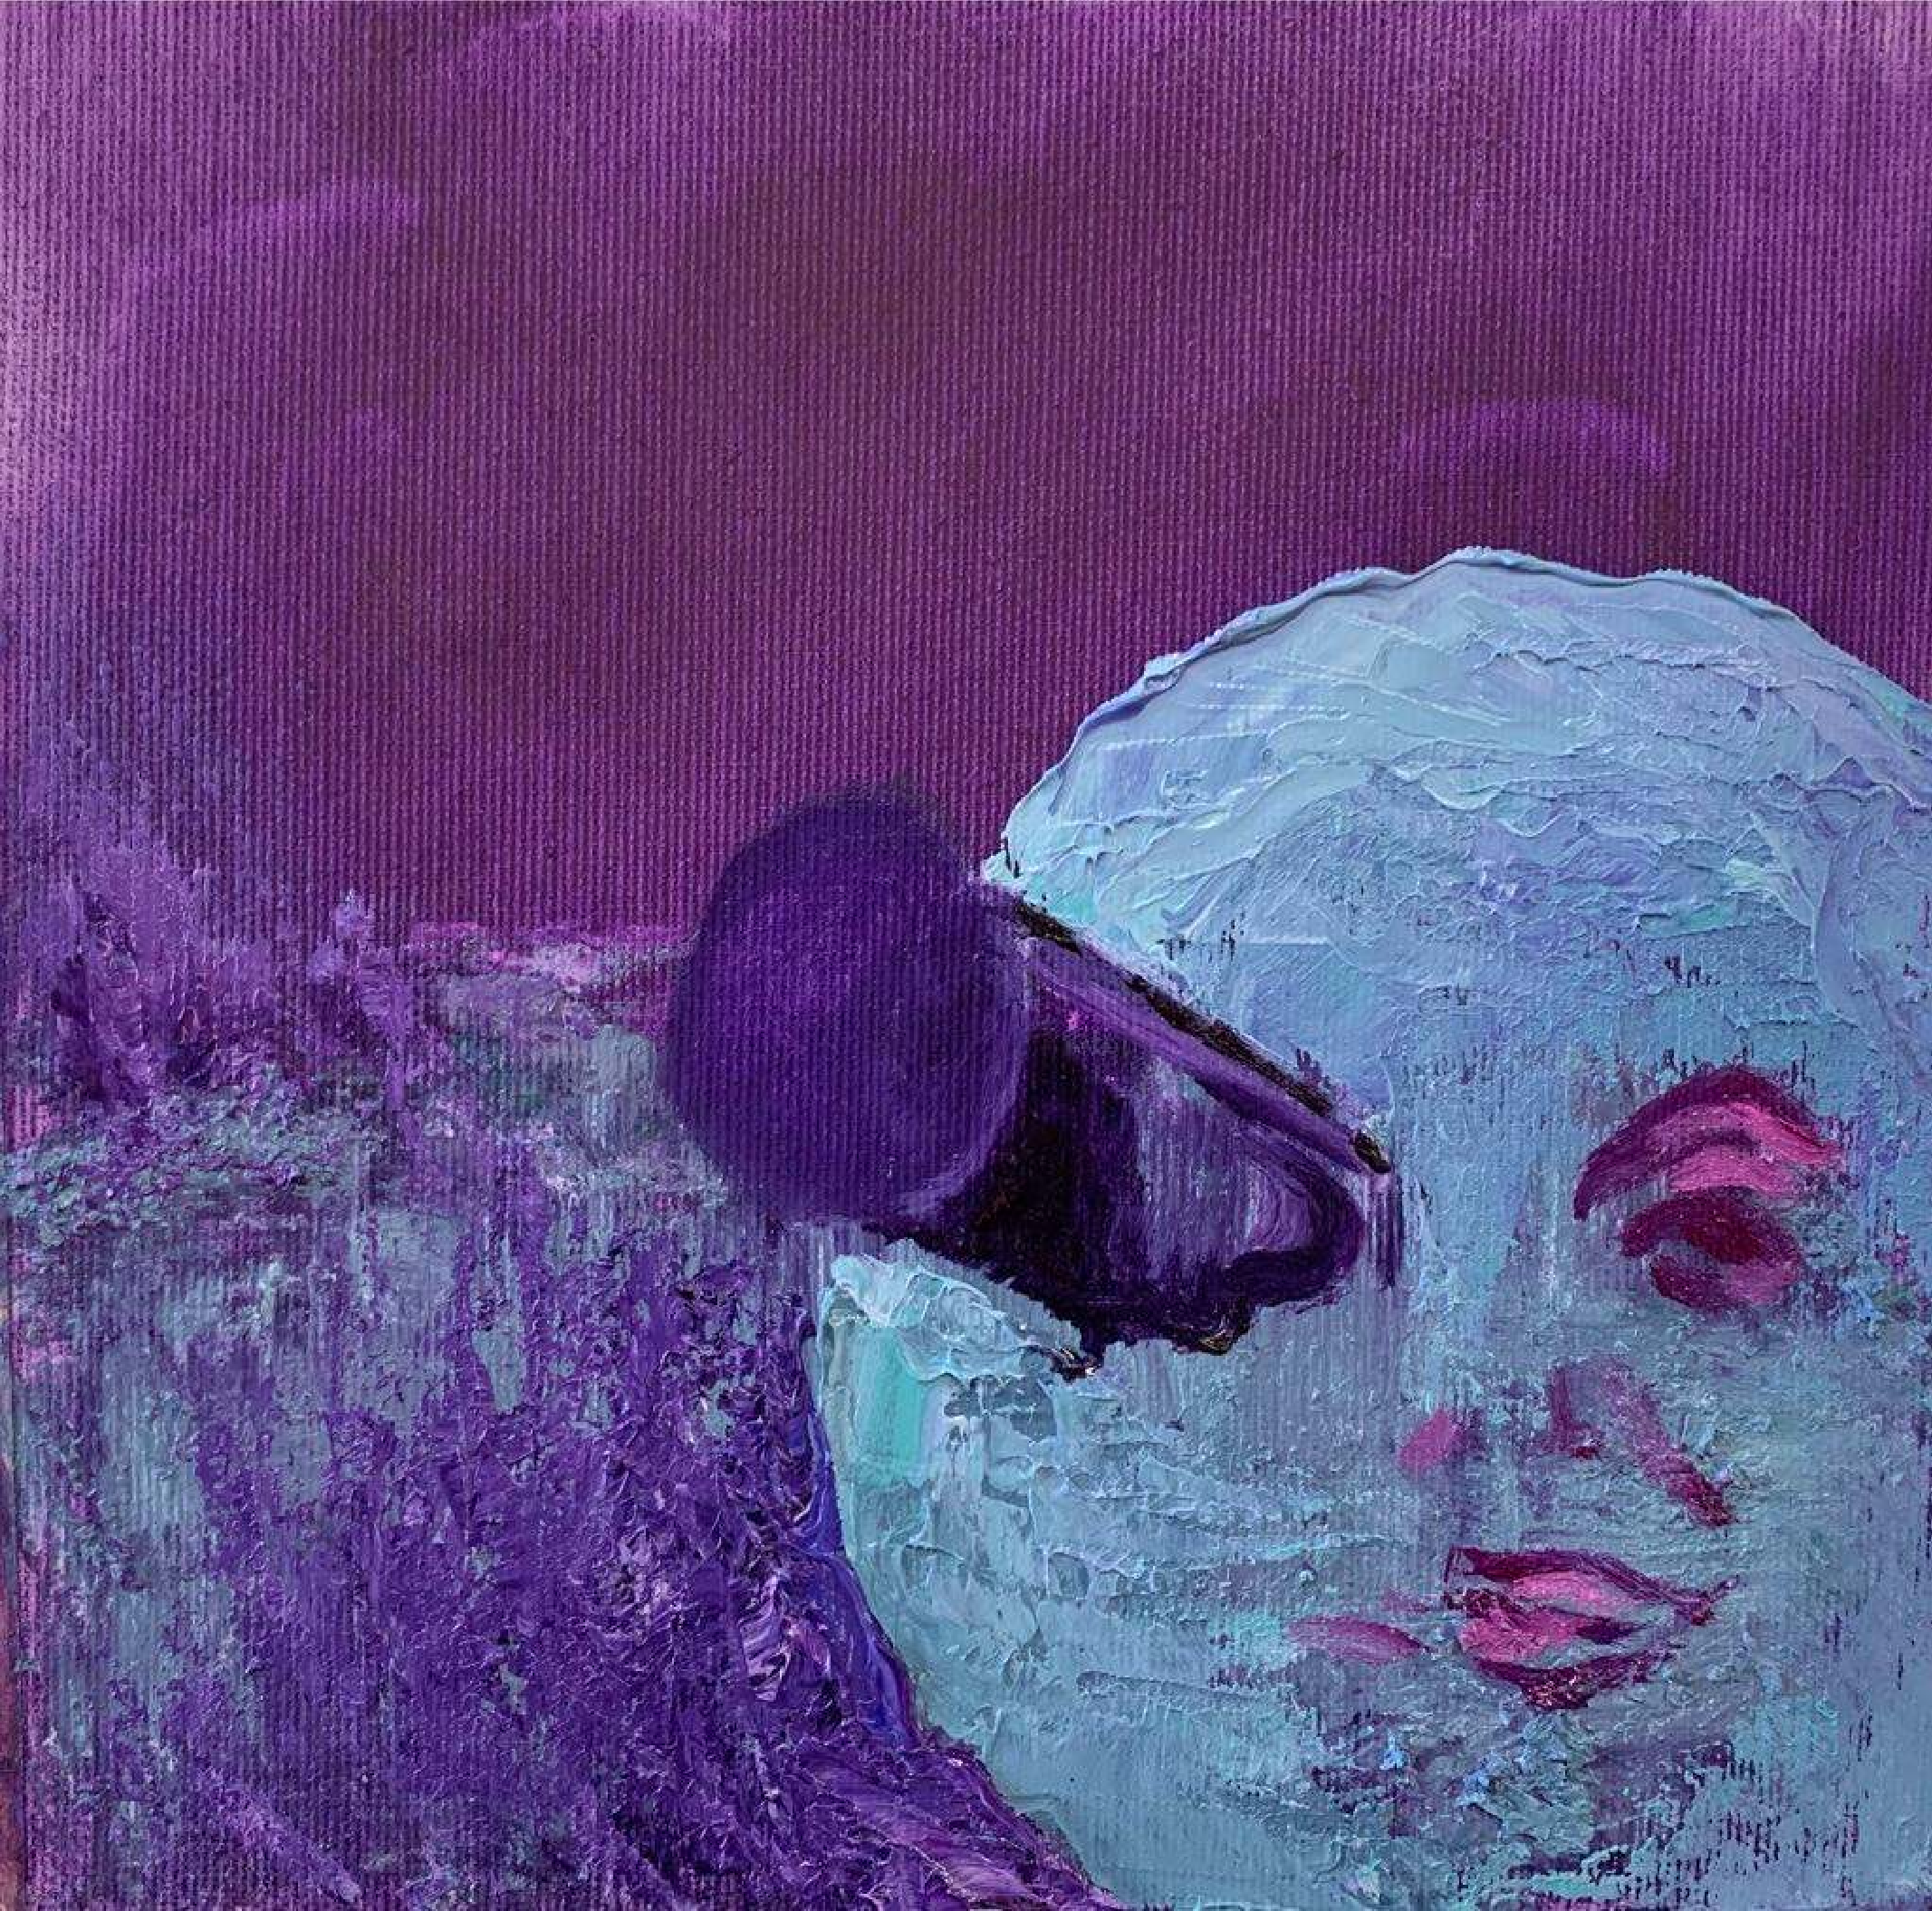
\includegraphics[height=1.98507in]{figuras/boudet-cena-melies.pdf.compressed.pdf}
	\figurenote{\series{Fora de Campo}. Tratamento com restos de tinta da paleta. Foto da autora}
\end{minipage}
\end{figure}


\paragraph{\emph{Frames} de filmes} Com o objetivo de aproximar a experiência do cinema à da
pintura, explorei alguns assuntos por meio de \emph{frames} de filmes.
Em consequência, avaliei que um dos eixos, o Olhar, abrangia os demais.
Iniciou-se então uma reconfiguração nos títulos das series dos esboços
e posteriormente das obras em finalização. O termo \emph{olhar} ou
\emph{olhar do cinema} transformou-se na matriz principal para os
esboços subsequentes, que subdividiram em três: \emph{movimento, humano
	em frames e cenário no cinema/espaço profundo}. Este Projeto que também
dava nome à série de esboços \emph{Olhar do cinema}, passou a se
desenvolver paralelamente ao Projeto \emph{O balanço}, que também fazia
referência ao conceito de movimento, só de uma outra forma. Este novo
viés da pesquisa é sobre a construção de uma pintura atravessada pelo
olhar de uma câmera em movimento.

Como já descrito no \cref{cap2-impacto-evolucao-otica}, a palavra
movimento se apresenta sempre que tentamos associar a imagem na pintura
figurativa à do cinema: \emph{impressão de movimento}. A experiência
com o objeto mala em pintura, além de contemplar a questão do movimento
e deslocamento, de um ponto de vista metafórico, apontava também para
um terceiro problema, que é o da \emph{memória do artista}. Além do ir
e vir das imagens mentais que ora estão mais próximas, ora mais
distantes, remete à prática de olhar de perto e olhar de longe comum a
muitos artistas durante o ato de pintar.

\begin{figure}
  \caption{Esboço referência Homem com uma câmera de Dziga Vertov}\label{esboco-dziga-vertov}

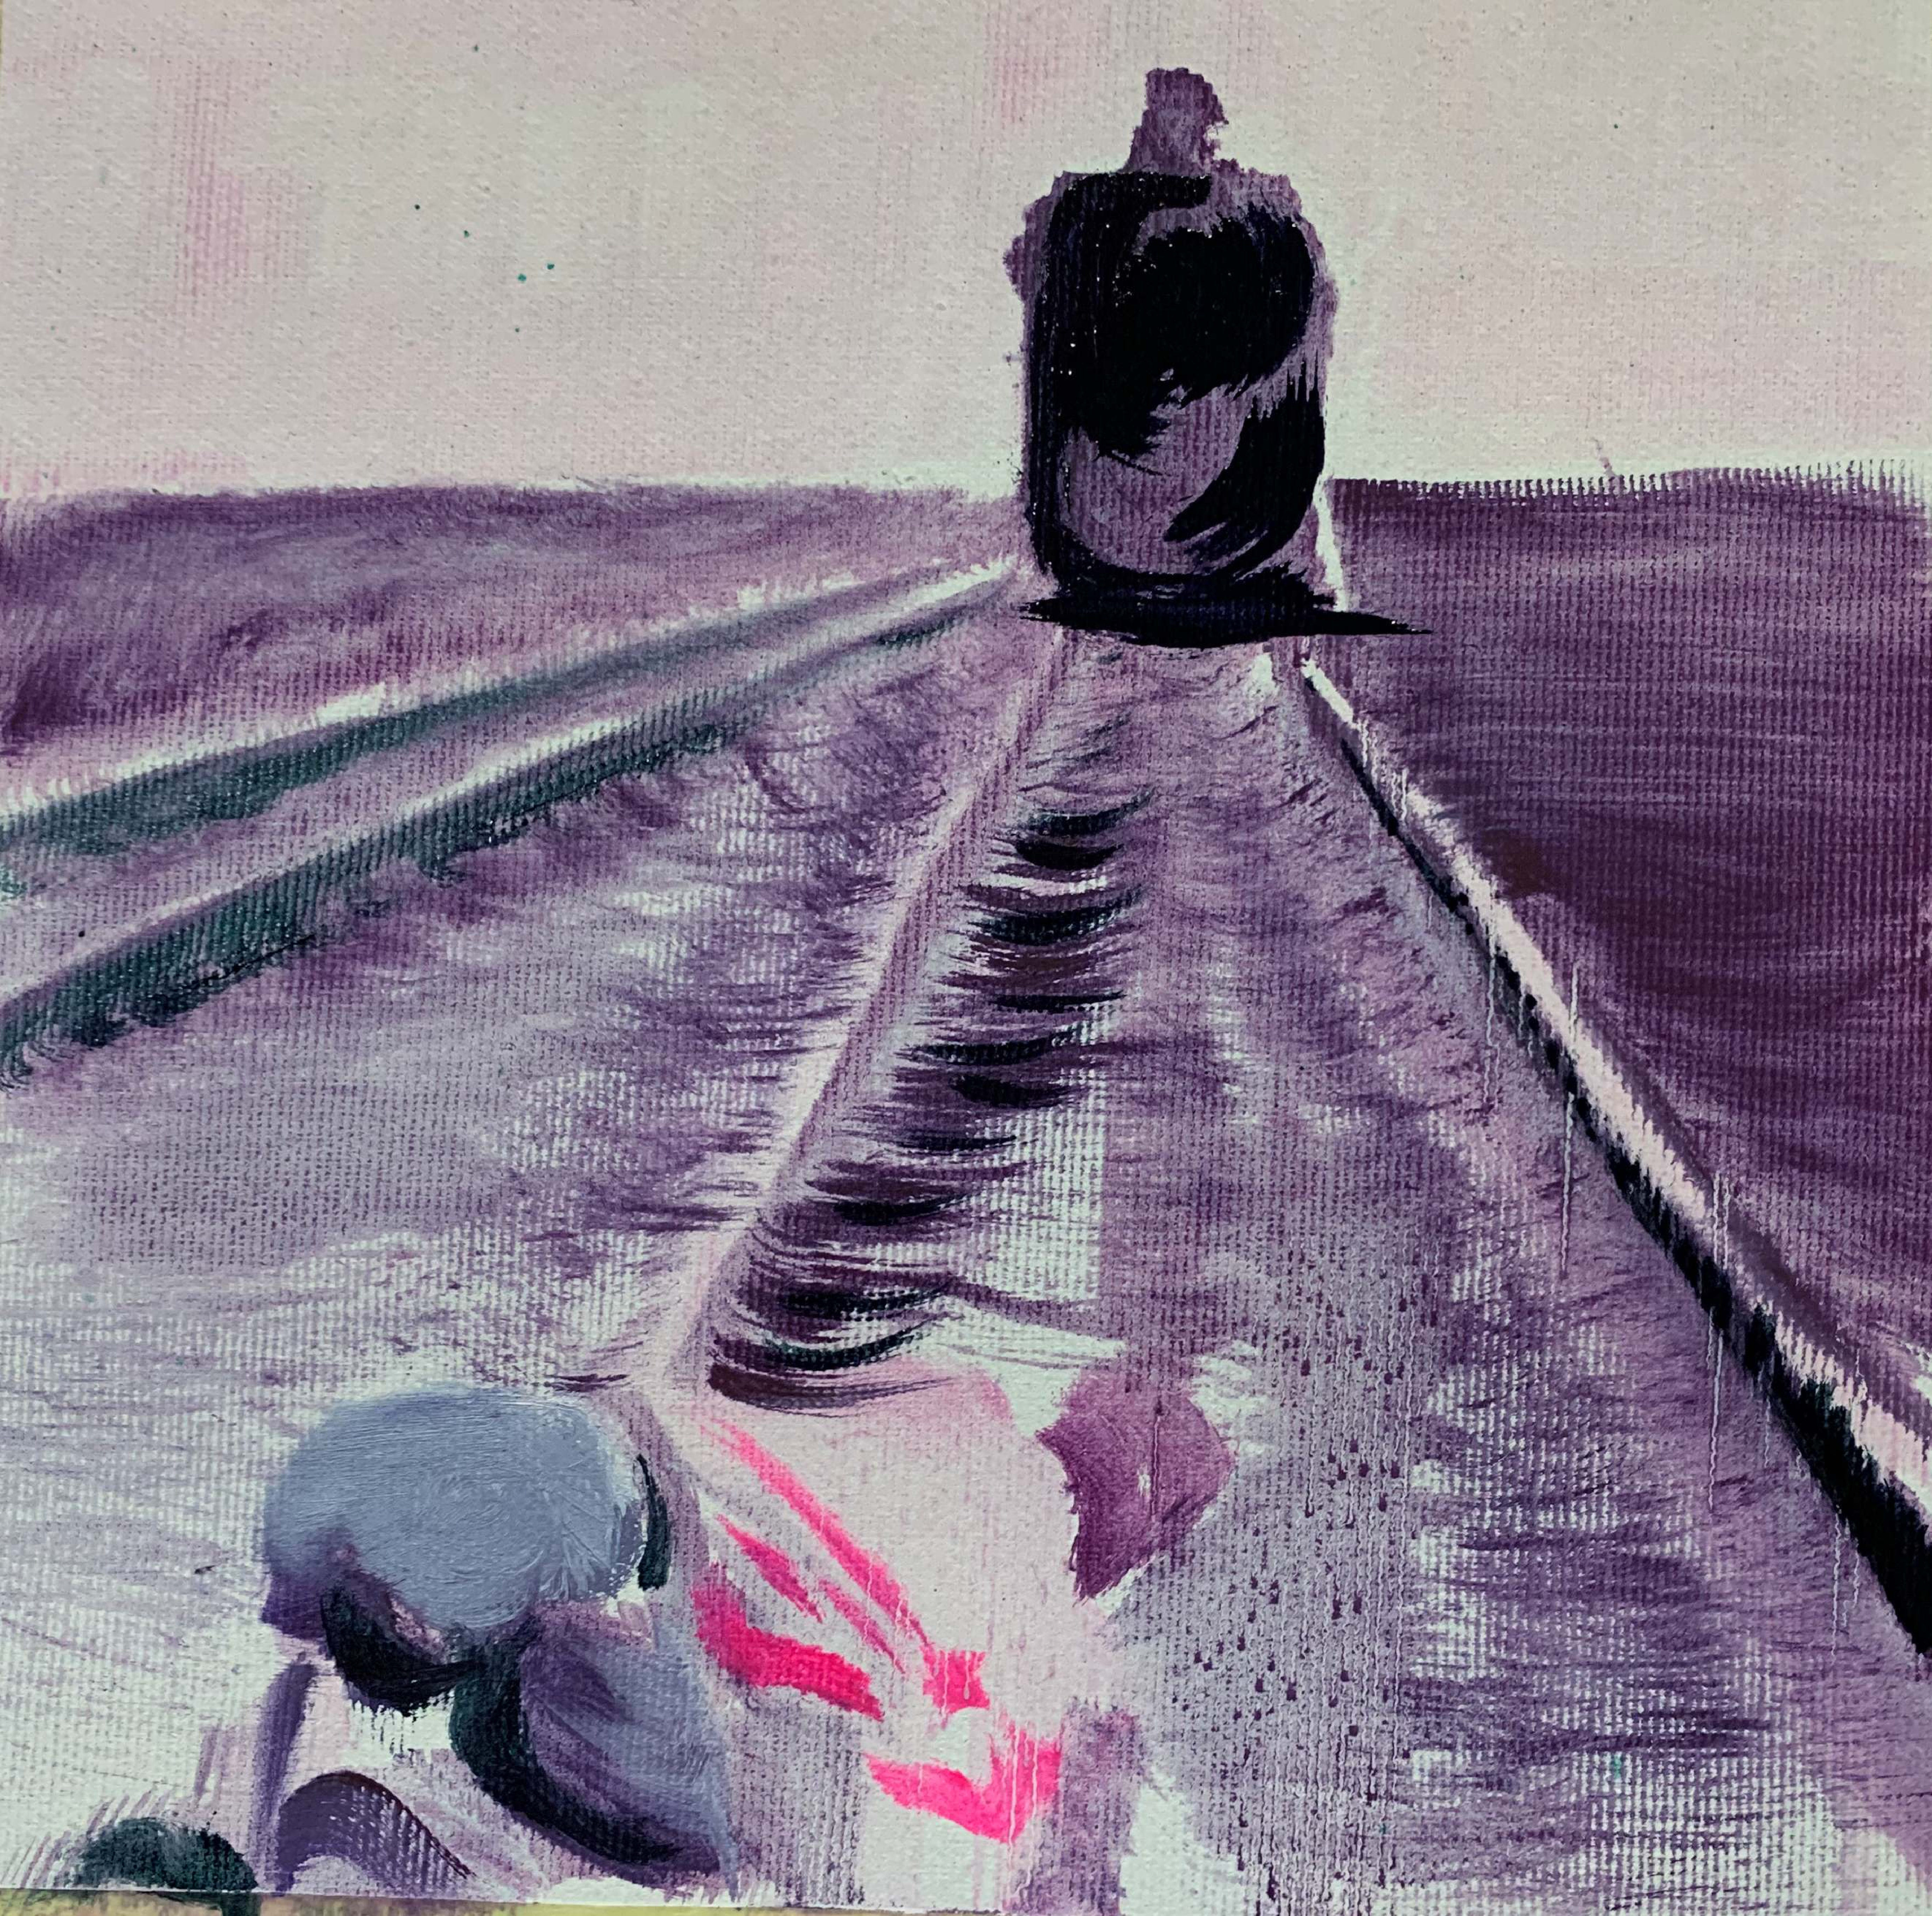
\includegraphics[width=1.65432in,height=1.61402in]{figuras/esboco-referencia-homem-camera.pdf.compressed.pdf}
\end{figure}

As pesquisas relacionadas ao \emph{objeto} na pintura, que antecederam
o início deste mestrado, tinham origem nos planos próximos viabilizados
pela câmera de filmar. Da mesma forma, as possibilidades de
enquadramentos e ângulos utilizados nas fotografias de referência
ditavam as escolhas de cortes para posicionamento destes \emph{objetos}
na tela da pintura. As temáticas se sucederam, mas a ideia continua
sendo a mesma, uma preocupação em criar um \emph{cenário} com base na
imagem construída pelas lentes de uma câmera. Neste sentido, encontrei
na estética do \emph{Cinema olho} e do filme \emph{O Homem com uma
câmera} (\cref{esboco-dziga-vertov}), de Dziga Vertov uma referência importante. A série
\emph{Humano} se materializou por meio de um esboço inspirado neste
filme. O esboço se transformou em trabalho final.


Com \emph{Hitchcock}, comecei a unir ideias importantes como o
posicionamento da câmera, o fora de campo e a progressão visual de
Block (uma coisa que se transforma em outra) e o \emph{fora de campo}.
Percebi que a tônica sobre a questão do espaço, invadiu a pintura. Foi
preciso revisar os conceitos das séries dentro do projeto expositivo.
Mas enquanto não aprofundava termos da narrativa visual como espaço
plano, espaço profundo e espaço fora de campo, por meio de novas
sequências de trabalhos, as pinturas \emph{Vertigo I, II e III}
permaneceram na série \emph{Humano em frames}.

\begin{figure}
  \begin{minipage}{.3\linewidth}
  \caption{\artname{\odette}{Vertigo I}{2022} \phantom{aaaaaaa}}

	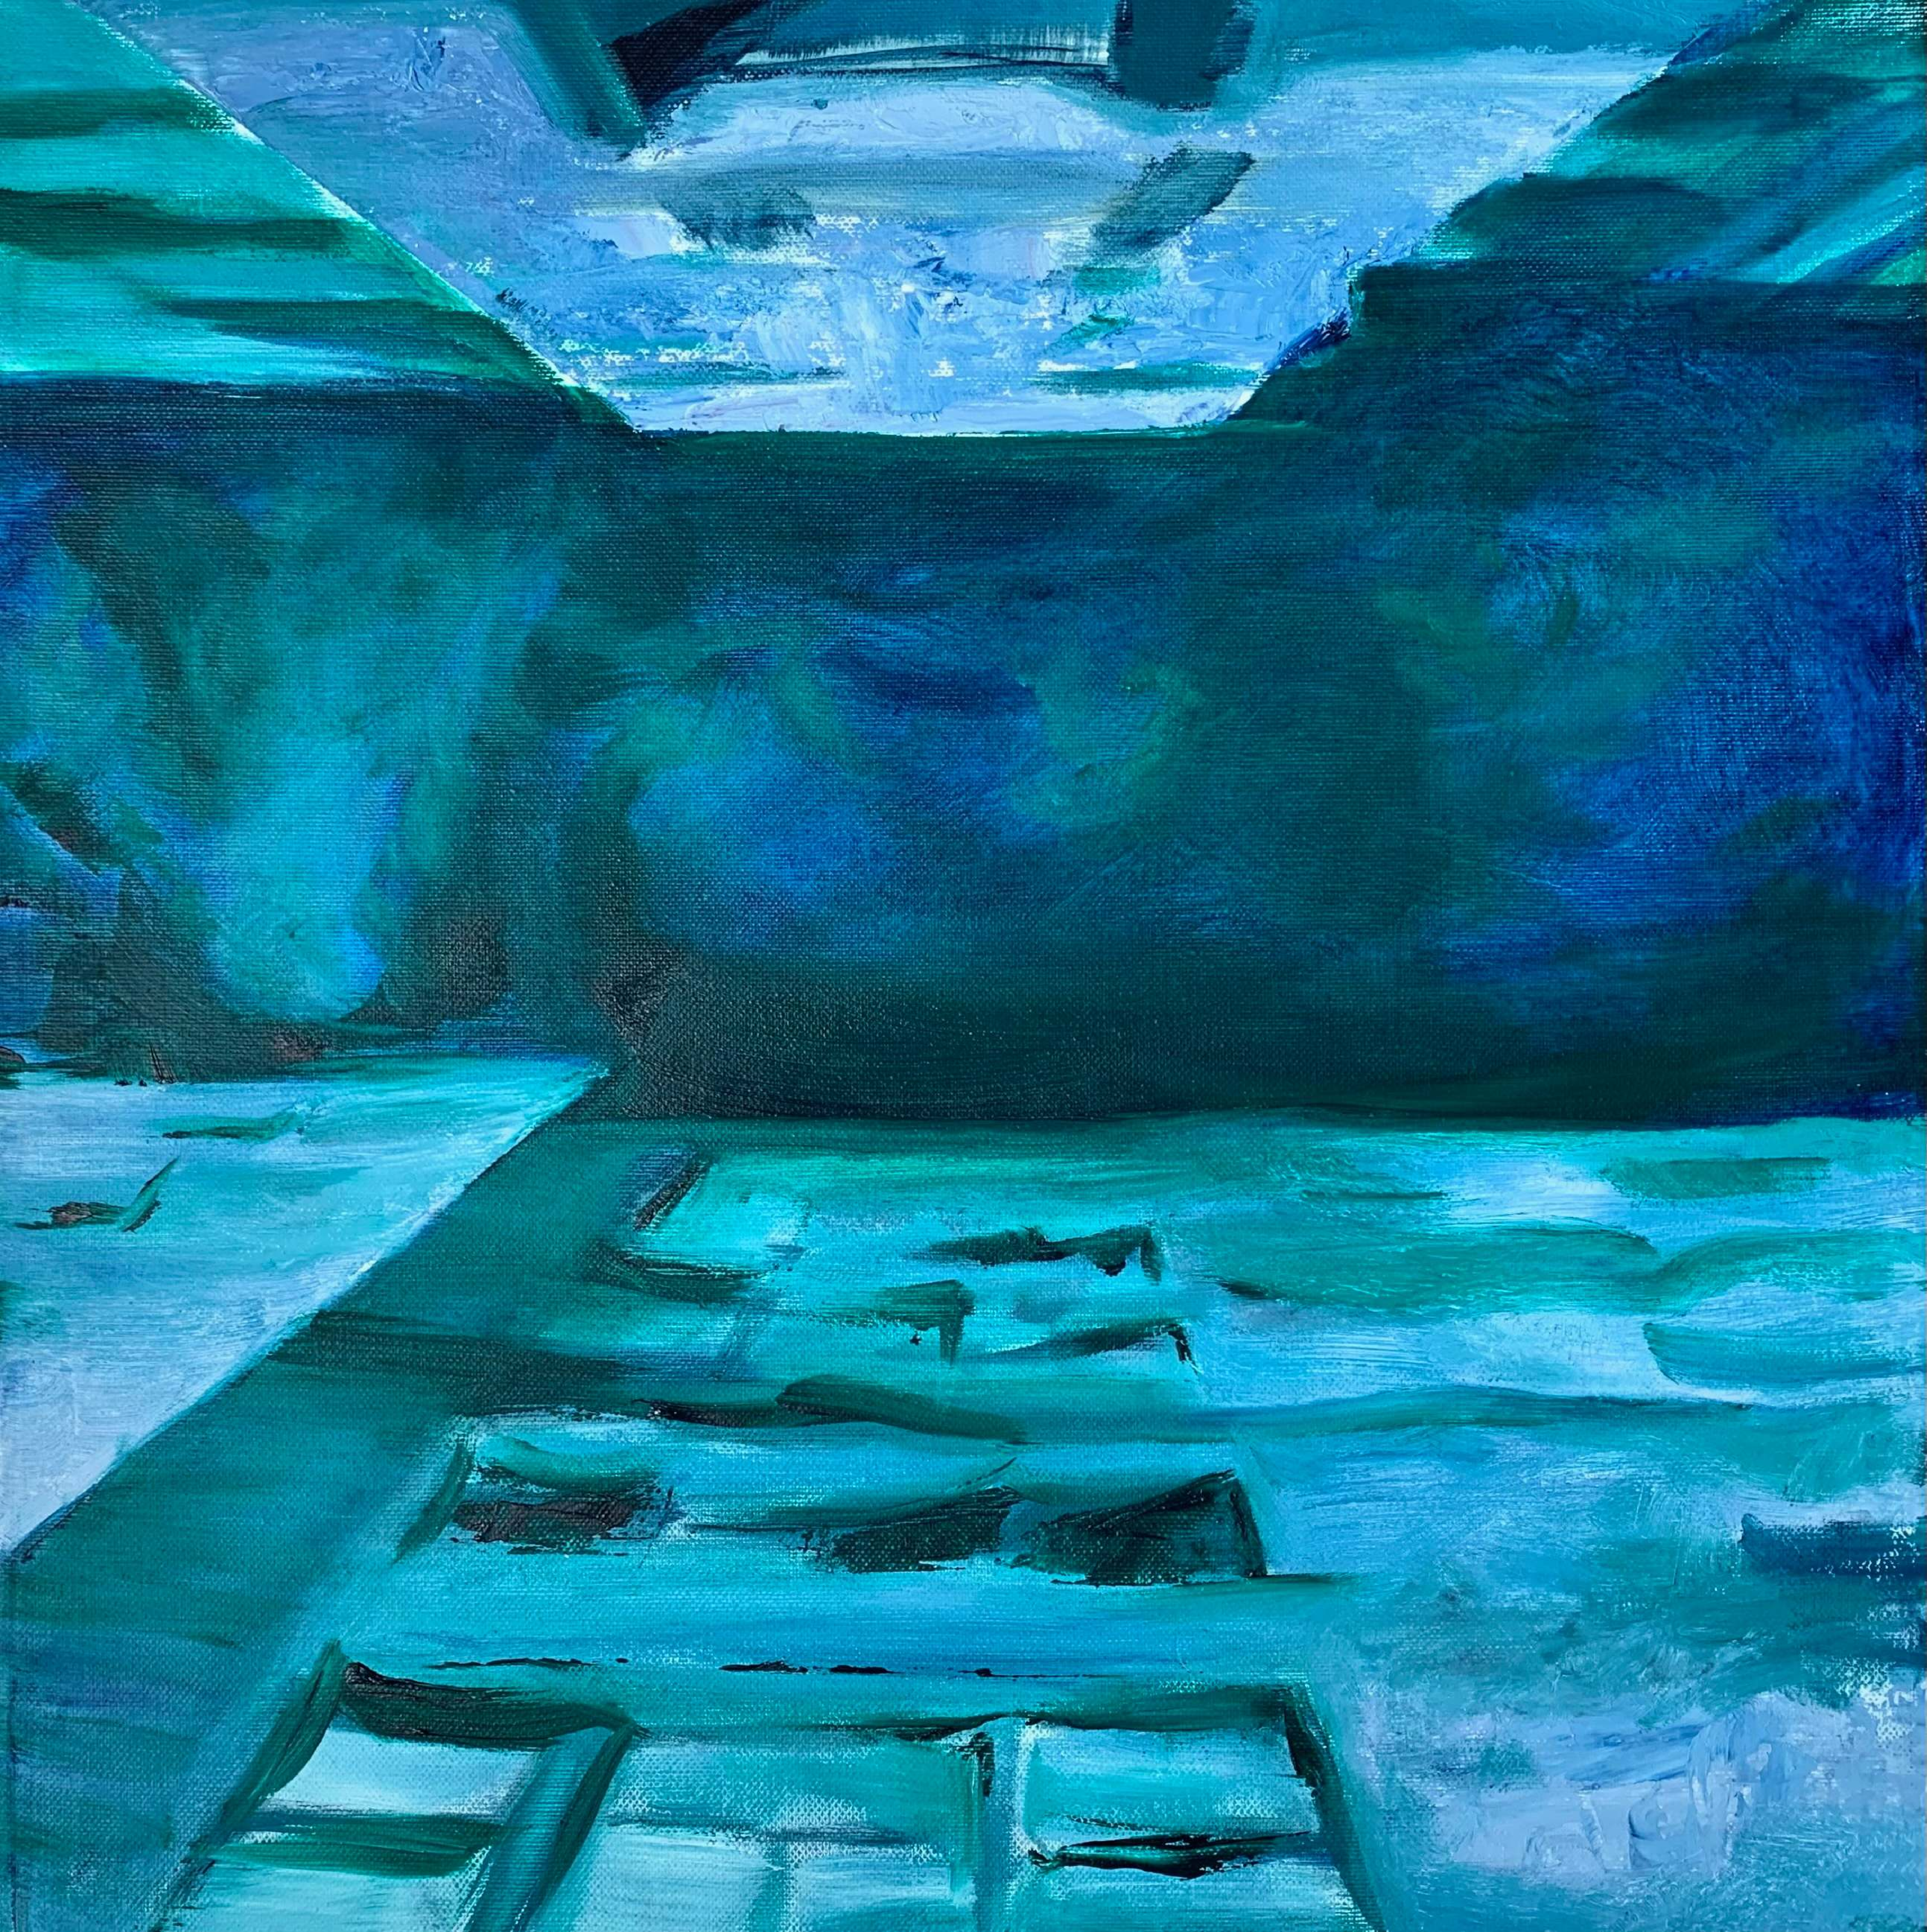
\includegraphics[width=1.77199in,height=1.77679in]{figuras/boudet-vertigo-I-2022.pdf.compressed.pdf}
	\figurenote{\series{Humano em frames}. \oleolinho. \artsize{40x40x3.5}}
\end{minipage}\hfill
\begin{minipage}{.3\linewidth}
	\caption{\artname{\odette}{Vertigo II}{2022}}

	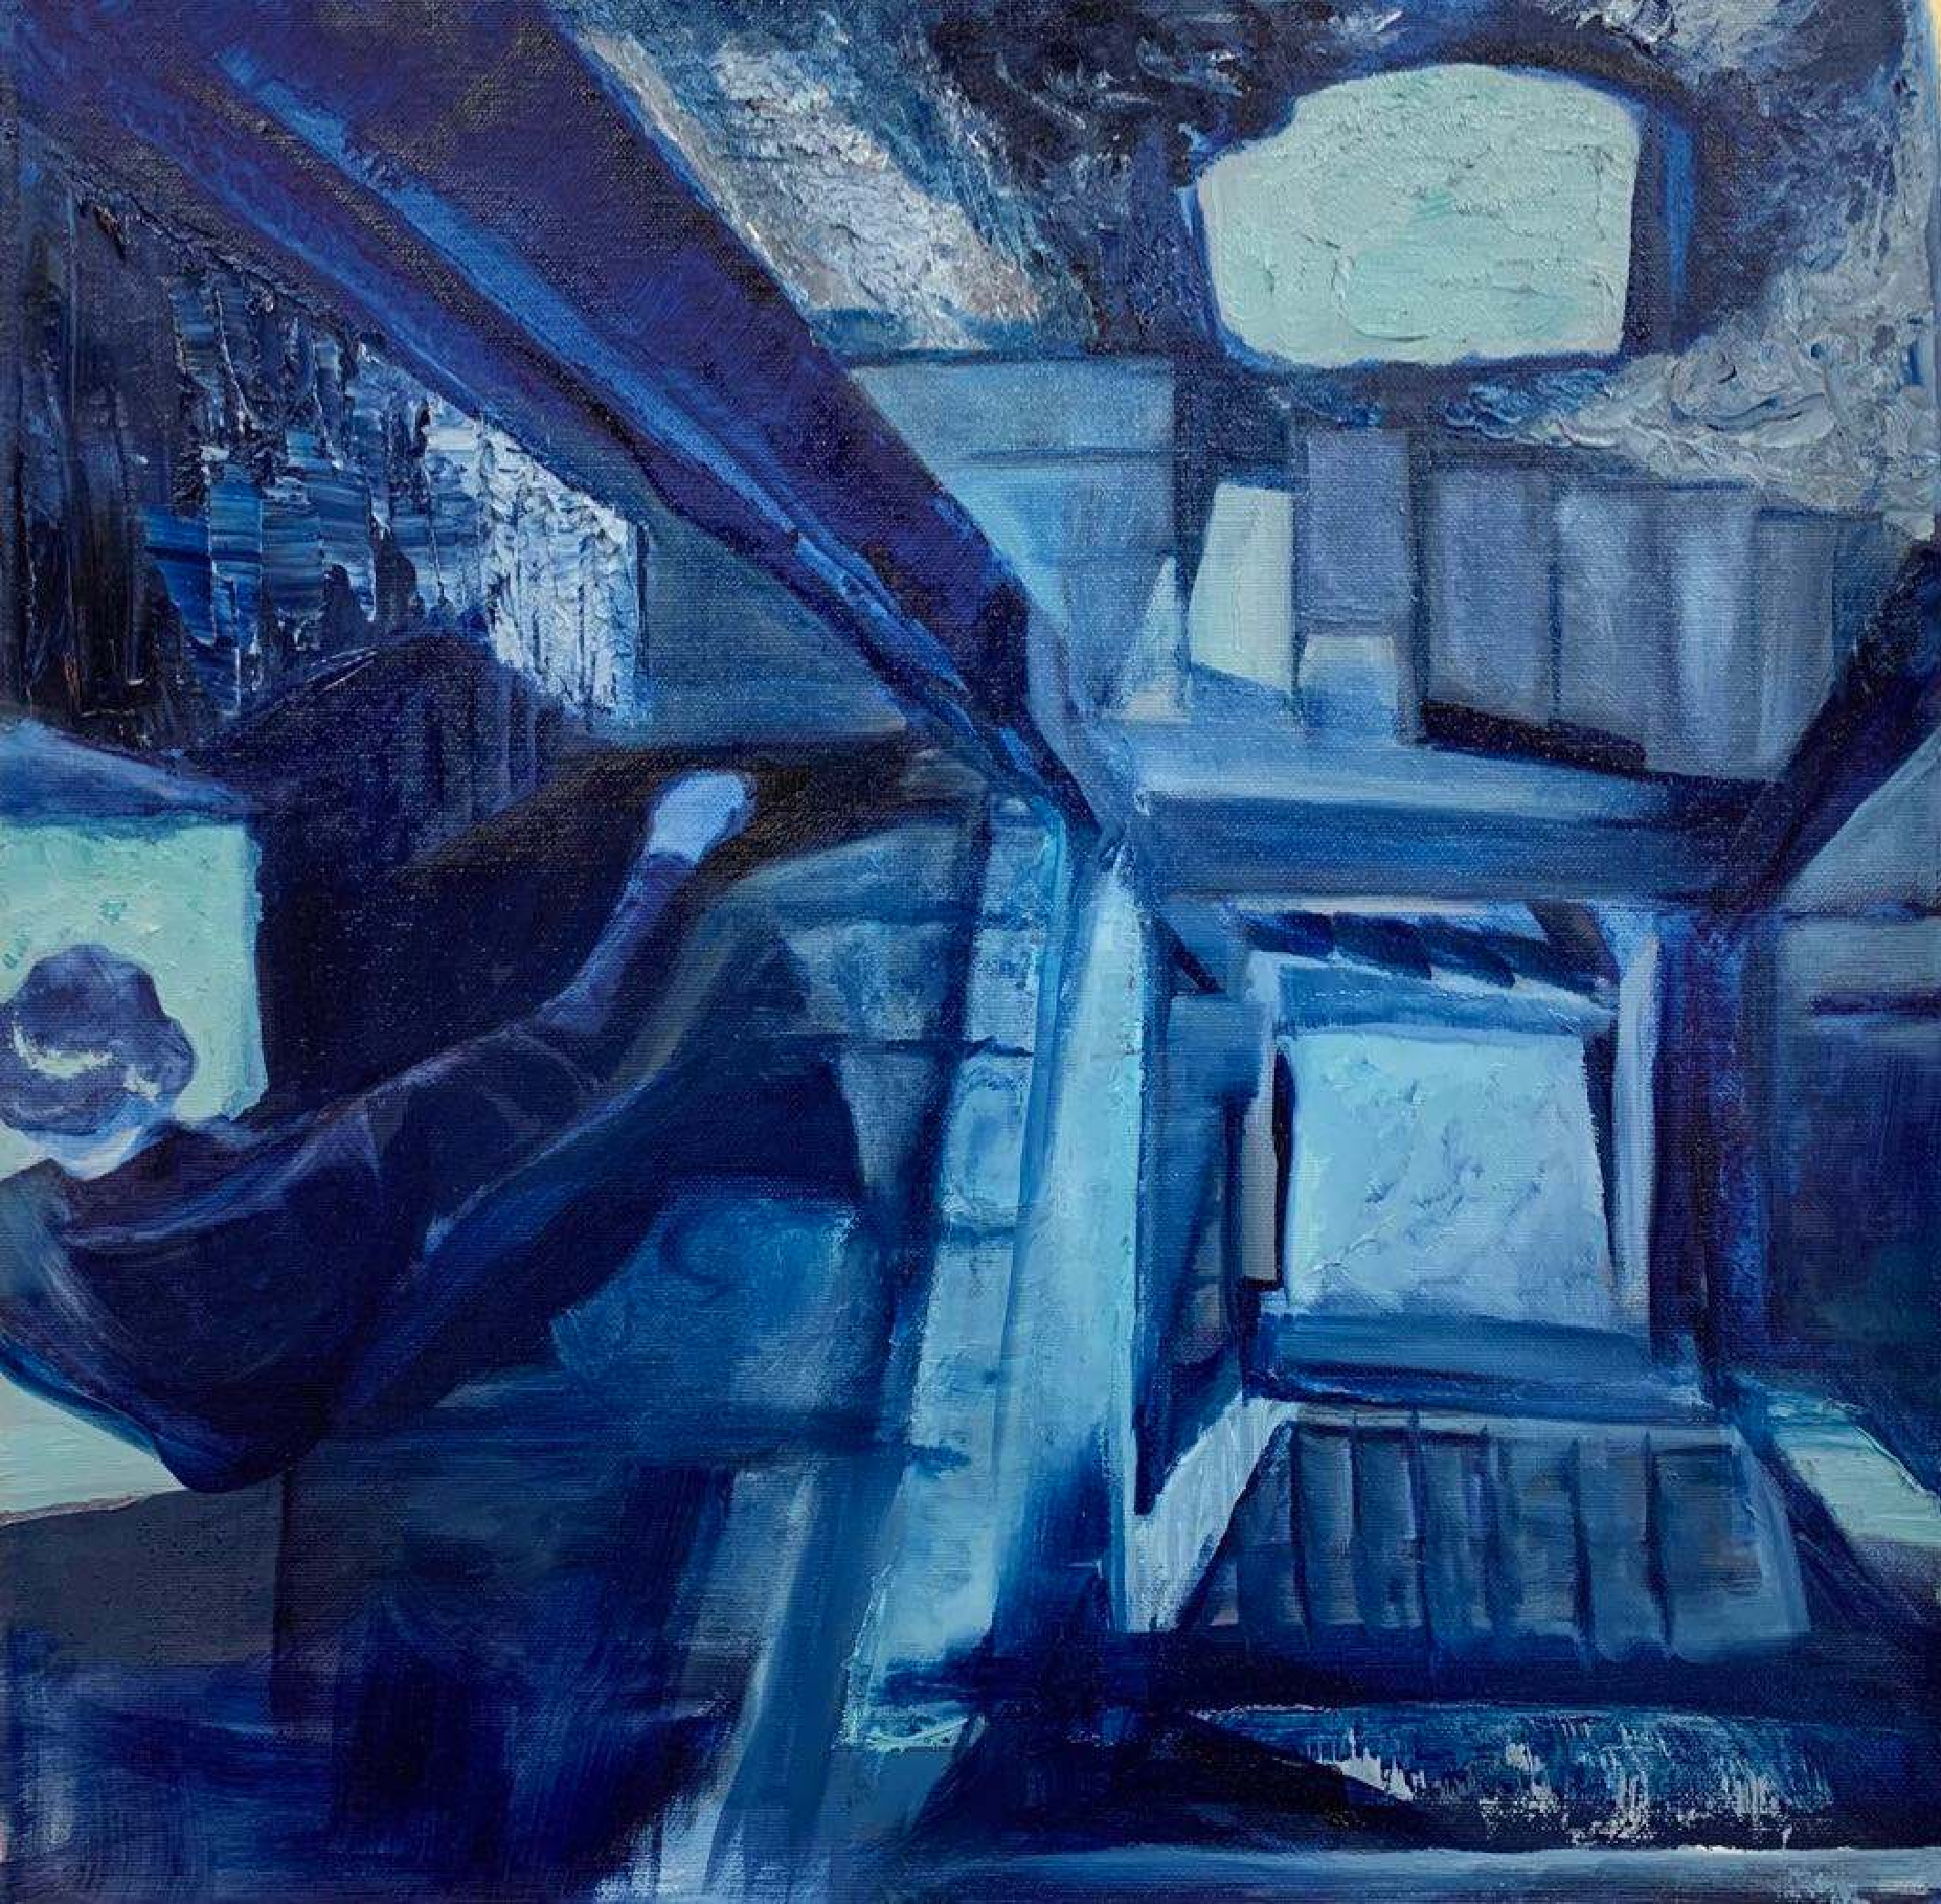
\includegraphics[width=1.8125in,height=1.77709in]{figuras/boudet-vertigo-II-2022.pdf.compressed.pdf}
	\figurenote{\series{Humano em frames}. \oleolinho. \artsize{40x40x3.5}}
\end{minipage}\hfill
\begin{minipage}{.3\linewidth}
	\caption{\artname{\odette}{Vertigo III}{2022}}

	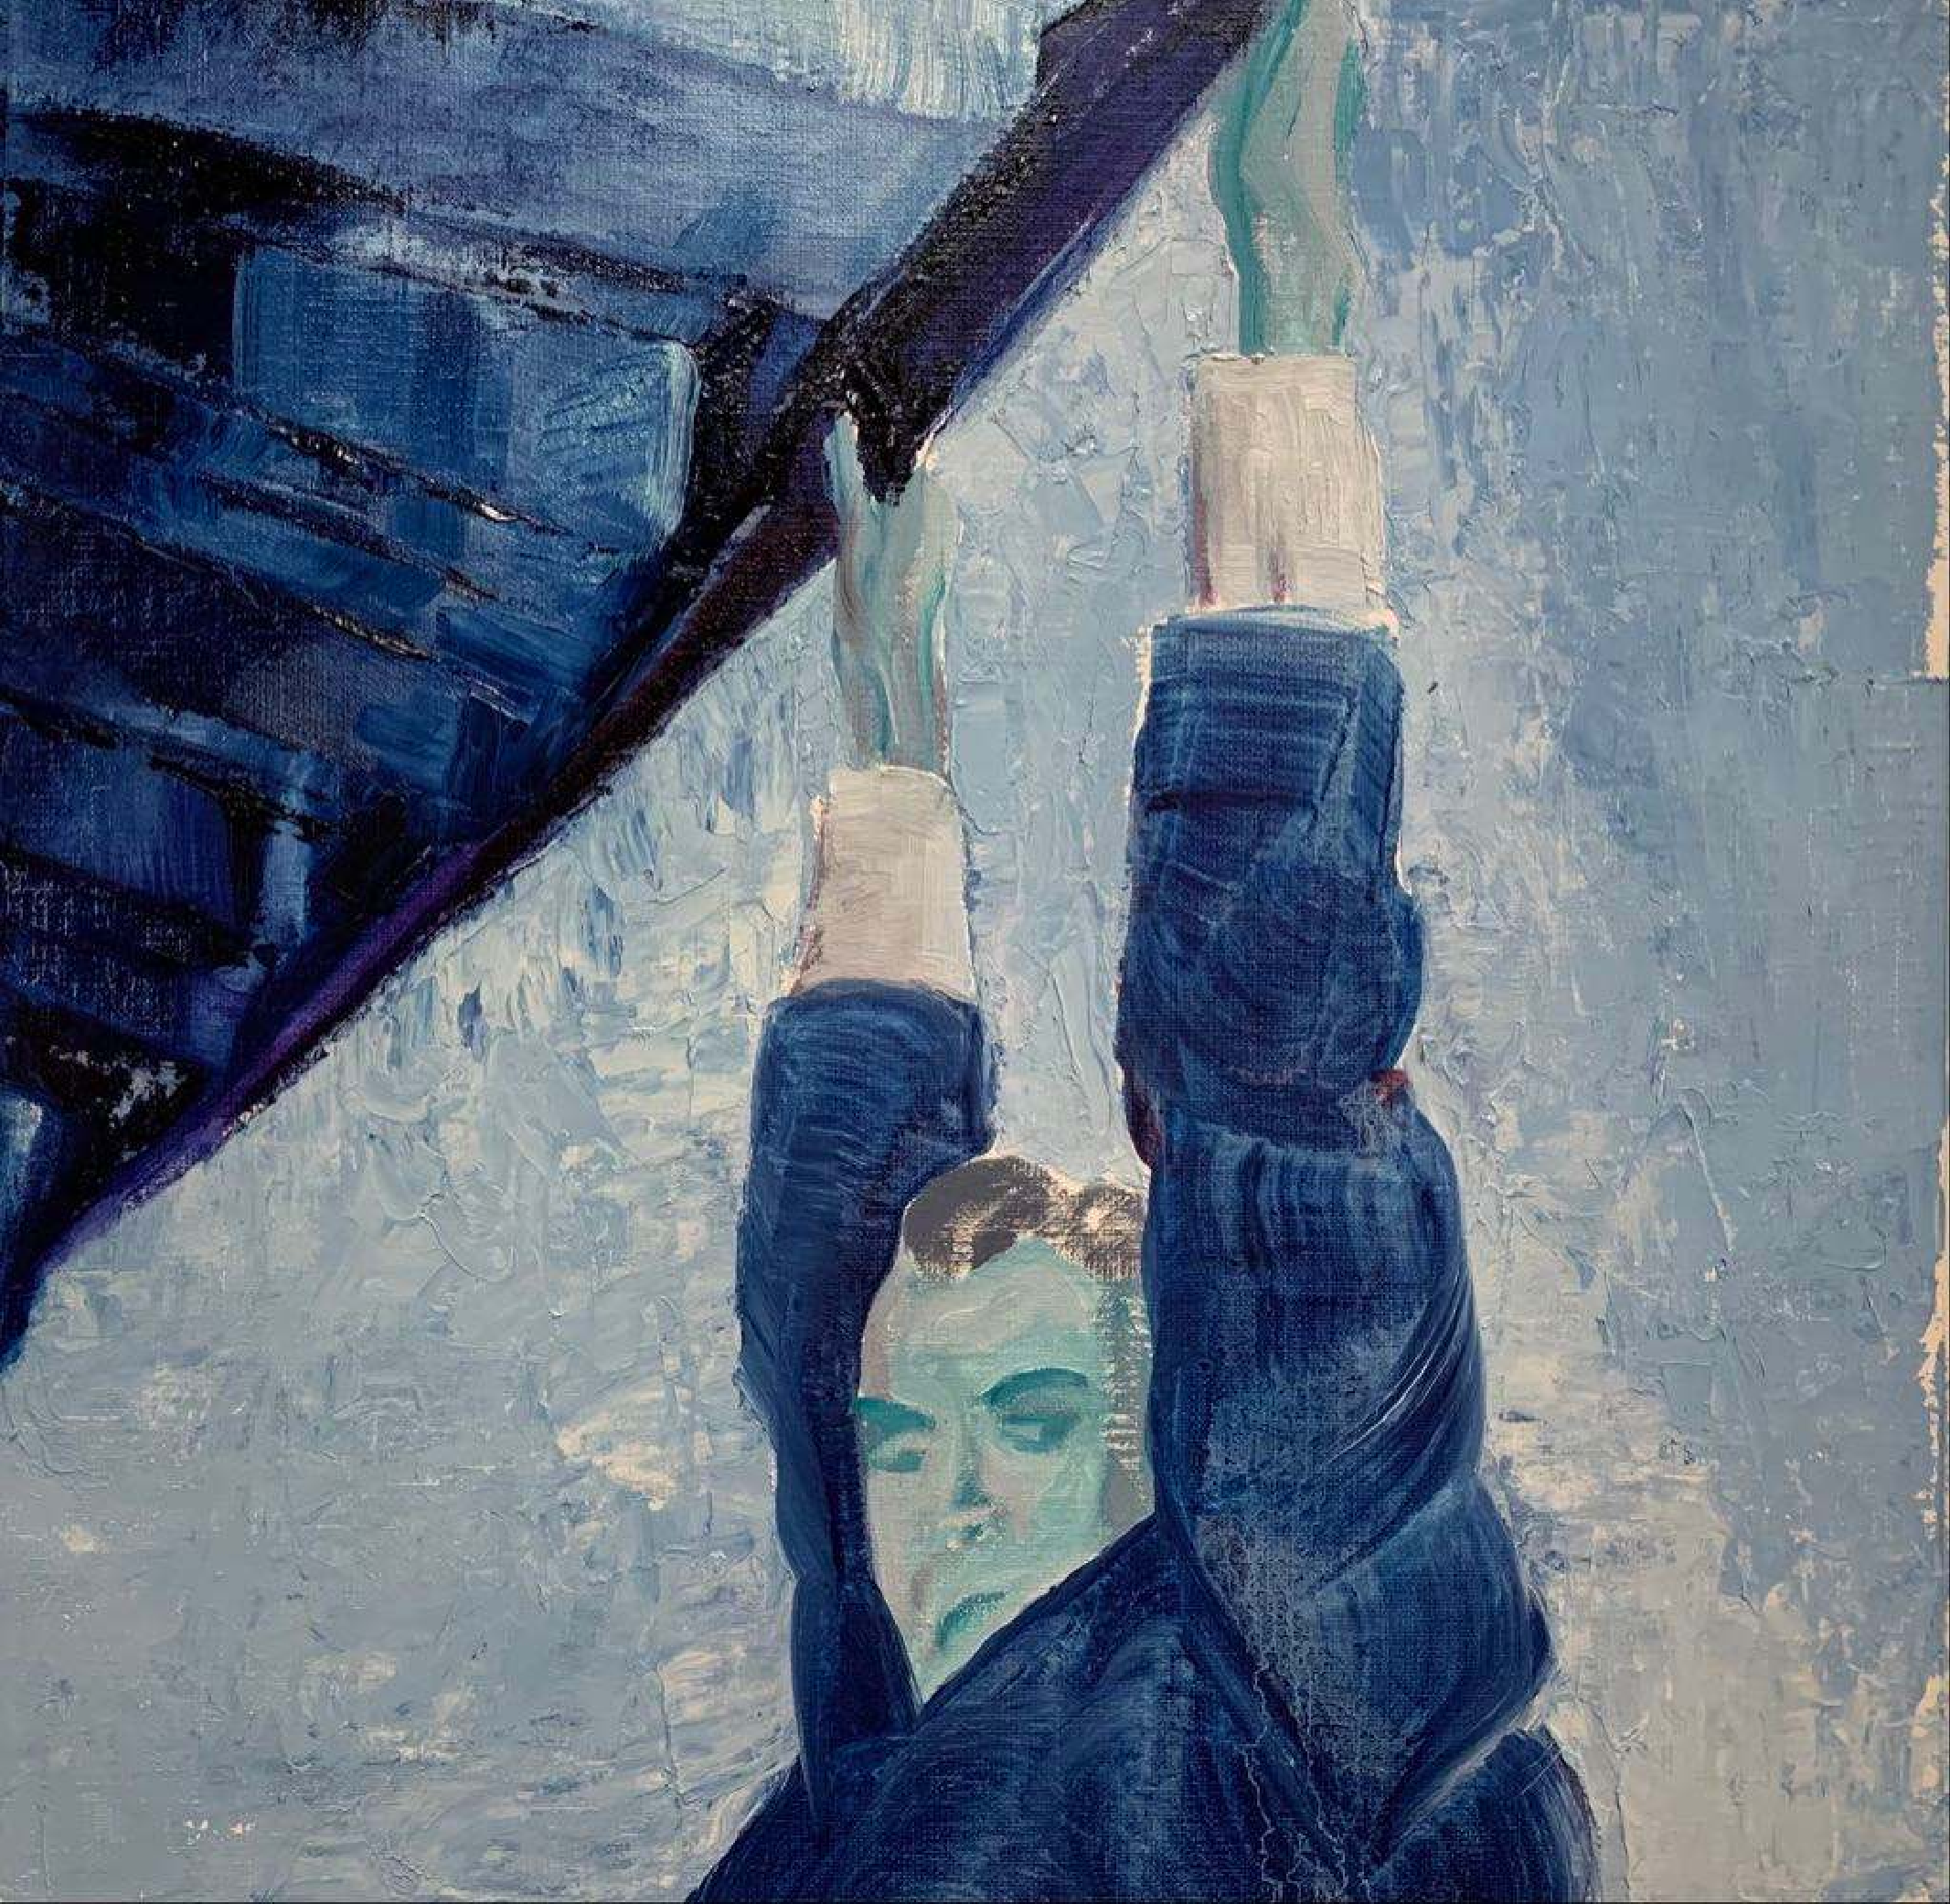
\includegraphics[width=1.81045in,height=1.76806in]{figuras/boudet-vertigo-III-2022.pdf.compressed.pdf}
	\figurenote{\series{Humano em frames}. \oleolinho. \artsize{40x40x3.5}}
\end{minipage}
\end{figure}

O \emph{personagem} da mala fechada, frequentemente o único elemento da
cena, serviu ao objetivo de representar possíveis significados poéticos
e metafóricos com diferentes abordagens. Agora é preciso afinar o
projeto expositivo a linhas de pensamento voltadas para estruturar a
narrativa visual do filme, tal qual orienta Block.

As ramificações das teias deste universo se expandem e contraem, e
\textcite{deleuze2004imagem} traz a ideia das imagens rarefeitas e
esvaziadas.

\begin{displaycquote}[22-23]{deleuze2004imagem}[.]
	\textelp{} imagens rarefeitas são produzidas, seja quando toda a tônica é
	posta num só objeto (em Hitchcock, o copo de leite iluminado do
	interior, em \emph{Suspicion}\footnote{Filme Suspeita (1941)}, a brasa
	do cigarro no retângulo negro da janela, em \emph{Rear
		Window}\footnote{Filme Janela indiscreta (1954)}), seja quando o
	conjunto está vazio de certos subconjuntos (as paisagens desertas de
	Antonioni, os interiores esvaziados de Ozu). O máximo de rarefação
	parece atingido com o conjunto vazio, quando o ecrã aparece todo preto
	ou todo branco. Hitchcock dá um exemplo em \emph{Spellbound}\footnote{Filme
		A Casa Encantada (1945)}, quando um outro copo de leite invade o ecrā,
	deixando apenas uma imagem branca vazia. Mas, das duas vezes, rarefação
	ou saturação, o quadro ensina-nos assim como a imagem não nos dá apenas
	a ver. Ela é tao legível como visível
\end{displaycquote}

Com isto, intuí que a forma figurativa deveria dar um passo atrás e
sair de campo, oferecendo espaço para \emph{conceitos}. No
\emph{Capítulo Quadro e Plano, Enquadramento e Décupage}, ele segue:

\begin{displaycquote}[25]{deleuze2004imagem}[.]
	\textelp{} É sobre o \emph{principal e o secundário}\ldots\ O quadro é, pois,
	inseparável de duas tendências, à saturação ou à rarefação. Sobretudo o
	grande ecrã e a \emph{profundidade de campo} permitiram multiplicar os
	dados independentes ao ponto que uma cena secundária aparece na frente,
	enquanto o principal se passa no fundo (Wyler), ou que já não se pode
	fazer uma diferença entre o principal e o secundário (Altman)
\end{displaycquote}

Criei o título da série \emph{Espaço no ecrã}, que abrigou o termo
\emph{profundidade de campo}. Com a possibilidade de trabalhar o espaço
arquitetônico ainda rarefeito, sinalizando aos poucos o espaço
profundo, apto a receber alguns elementos para compor uma narrativa.
Desta forma, me conectei a conceitos estéticos cinematográficos de Ozu
(1903--1963). Segundo \textcite{dias2016riso}, a essência do cinema
utilizada por Ozu, explica a frequente qualificação de seus filmes
contemplativos como \emph{poéticos}. Para ele, a estética das imagens
de Ozu são o resultado de três fatores de ordem formal.

\begin{displaycquote}[136-137]{dias2016riso}[.]
	Em primeiro lugar, o rigoroso sentido de composição de cada plano,
	\textelp{} o geometrismo dessa composição, dos enquadramentos dos planos,
	de interiores e de exteriores \textelp{}. Toda uma \emph{picturalidade} da
	cine-imagem, toda uma infinita aproximação \emph{ozuiana} do cinema e da
	pintura, mas para assim afirmar a infinita distância entre os dois
	tipos, pictórico e cinematográfico, de imagens
\end{displaycquote}

A câmera quase sempre fixa e seu posicionamento oblíquo, evidenciaria
um efeito de profundidade de campo, e um distanciamento contemplativo,
aproximando assim a percepção do contemplador de pintura à do
espectador do filme. \enquote{De resto, o próprio Ozu declarava que o
	movimento é um atributo da câmera, mas \emph{não} do cinema\ldots\ O
	cinema de Ozu é, nisso, perfeitamente clássico, um cinema de montagem}
\parencite[138]{dias2016riso}. Os planos fixos, estáticos, por si só já
contam a história da pintura e do filme.

Pela observação dos aspectos analisados neste Capítulo, conclui-se que
o desenvolvimento do projeto deve muito à criação de uma metodologia
para registrar as ramificações relacionadas à temática. Neste sentido,
foi importante trazer as investigações sobre o movimento metafórico das
figuras \emph{mala} e \emph{balanço}, com as quais também realizei
experimentos audiovisuais. Além disto, a revisão bibliográfica de
teorias do cinema durante a dissertação, abriu possibilidades de
abordar conceitos como o do espaço profundo, espaço plano, progressão
visual, princípio de afinidade e contraste, rarefação e saturação, como
base para de projetos pictóricos. Até o presente momento, os títulos
das séries e pinturas do projeto \emph{Olhar do cinema} se encontram
com a configuração abaixo:

\begin{enumerate}
	\item Série Consequências

    \begin{enumerate}[topsep = 0pt]
		      \def\labelenumi{\arabic{enumi}.}
		      \item Plongé e contre-plongée
		      \item Storyboard
		      \item Progressão visual
		      \item Princípio de afinidade e contraste
	      \end{enumerate}

	\item Série Espaço no ecrã

    \begin{enumerate}[topsep = 0pt]
		      \def\labelenumii{\arabic{enumii}.}
		      \item Espaço profundo e espaço plano
		      \item Profundidade de campo
		      \item Rarefação e saturação
	      \end{enumerate}
	\item Série Humano em frames

    \begin{enumerate}[topsep = 0pt]
		      \def\labelenumii{\arabic{enumii}.}
		      \item Dziga Vertov
		      \item Vertigo
		      \item Victor Erice
		      \item Truffaut
	      \end{enumerate}
	\item Série Cenário Fora de campo

    \begin{enumerate}[topsep = 0pt]
		      \def\labelenumii{\arabic{enumii}.}
		      \item Cena Méliès
		      \item Atlântico norte I e II
		      \item Atlântico sul I
	      \end{enumerate}
\end{enumerate}

\section{A cor}\label{a-cor}

Finalizo este capítulo descrevendo meu processo decisório pessoal
relacionado à cor. Os estudos de \emph{Notan}\footnote{Notan --
	definição. - www.virtualartacademy.com/notan/} ajudaram a pensar a
distribuição dos valores de claros e escuros na pintura, independente
dos matizes. A palavra japonesa \emph{Notan} significa \emph{escuro,
	claro}, derivada de \emph{Nong} (expresso, forte concentrado) e
\emph{Dan} (fraco, aguado). Refere-se à quantidade de luz refletida, ou
à massa de tons de diferentes valores. A técnica do \emph{Notan} me foi
apresentada nas aulas de pintura da Escola de Belas Artes da UFRJ em
2016, pela professora e artista Monique Queiroz (e serviu de apoio para
as primeiras pinturas no processo indireto, que realizei naquele
período. O \emph{Notan} como ferramenta de estudo da composição é
bastante útil para trabalhar com formas mais orgânicas, bem como para
realizar as primeiras camadas do processo indireto no estabelecimento
de valores.

Atualmente, antes de projetadas, as imagens de referência, são editadas
para excluir os matizes, permanecendo quase que somente o preto, o
branco e poucas tonalidades de cinza. Este processo é realizado
especialmente para os trabalhos em camadas e foi desencadeado pelos
estudos de Notan.

Mas como lidar com a cor no cinema e na pintura?

Embora a percepção das cores na pintura e no cinema pareça semelhante,
existem algumas diferenças a serem consideradas. O resultado da cor que
se vê em uma tela de pintura provém de uma luz refletida que atravessa
pigmentos e tinta. Já a luz que proporciona os diferentes matizes
percebidos em um ecrã de cinema, de celular ou de outros dispositivos
digitais é uma luz emitida e nos objetos eletrônicos são formadas por
adição. O sistema CMYK se baseia na pigmentação de \emph{Cyan, Magenta,
	Yellow e Black}. Neste sistema, objetos físicos como as telas de
pintura, as cores são reproduzidas através da subtração. Já no sistema
RGB, a luz é adicionada com níveis de cor desejados, formado pelas
cores \emph{Red, Green and Blue.}

Esta diferença pode se tornar um grande problema para os pintores mais
detalhistas, que trabalham com hiper-realismo, e para artistas gráficos
que dependem de uma alta precisão na reprodução das cores para produtos
impressos. No entanto sabemos que além do componente físico relacionado
à luz ambiente, sempre existirá uma diferença na percepção das cores de
acordo com o olhar do observador.

Existem muitos esquemas e teorias da cor à nossa disposição, que nem
sempre são suficientes para resolver o problema da articulação de
valores, matizes e cromas de forma a simplificar o trabalho do pintor.
A decisão sobre como escolher uma paleta para uma pintura, série ou
projeto pode se tornar algo bastante complexo. Por algum tempo utilizei
a teoria do \emph{Balão Cromático} (mencionado no Capítulo II) e dos
\emph{Contrastes} de Itten. Depois de muito pesquisar sobre os diversos
sistemas, esquemas e acordes de cor, ao longo da história da pintura,
adotei o quadro abaixo, disponibilizado pelo pintor Florence
Farges\emph{.} Em seus cursos de pintura on-line\footnote{Florent
	Farges www.florentfarges.com/the-art-and-practice-of-color/},
simplifica bastante para os artistas o modo como lidar com a matéria
das tintas e da cor.

\begin{figure}
	\caption{Teoria das Cores para artistas.}

	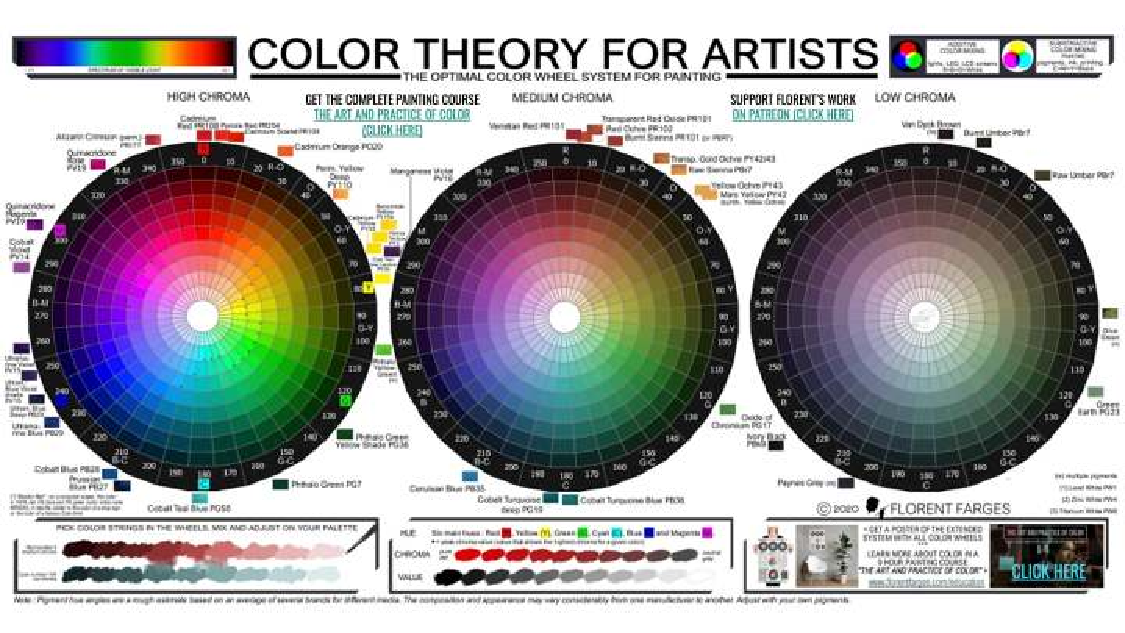
\includegraphics[width=4.7094in,height=2.64897in]{figuras/color-theory-for-artists.pdf.compressed.pdf}
	\figurenote{Fonte: \hiperlink{www.florentfarges.com/wp-content/uploads/2021/12/Color-Theory-for-Artists-Color-Wheel-System-1.pdf}{Florent Farges}}
\end{figure}

A professora de pintura \parencite{sabino2015pintura} revê a proposta de seu primeiro livro de
2000, já referenciado nesta dissertação, na forma abaixo:

\begin{displaycquote}[33]{sabino2015pintura}[.]
	o cerne da pintura poderia subsistir não na sua especificidade como
	médio ou na sua objetualidade, mas em algo mais imaterial, o que
	comparei a uma espécie de \enquote{configuração do olhar} que, antes da própria
	imagem do mundo e perante esta, fosse ela qual fosse, poderia atribuir a
	qualquer objeto visível características pictóricas e, assim, torná-lo em
	pintura ou, melhor ainda, fazer nele \enquote{acontecer} pintura
\end{displaycquote}

Após quinze anos da publicação de seu primeiro livro, ela declara
faltar-lhe algo mais fiável fisicamente, como a tinta.

Concluo que, por compartilhar desta visão pessoal de Isabel Sabino,
direcionei esta investigação no sentido de realizar uma pintura por
meio de estruturas visuais relacionadas ao cinema, e não o caminho
inverso. Acredito que não há nada mais importante para o ofício de um
pintor do que lidar com a fisicalidade da cor. Entretanto, o
encantamento com o mundo da tela preconizado por Hitchcock, no
\emph{voyeurismo} de \emph{A janela indiscreta (1954)}, e por com
milhares de narrativas fílmicas acumuladas ao longo da história do
cinema, me motiva a continuar buscando formas de conjugar estas duas
paixões. Paixões com as quais viajo não só para trás no tempo, à
procura de ensinamentos como os de \emph{Sargent} e \emph{Sorolla,} mas
também em busca de imaginar o futuro. Para mim, enquanto artista, é
fundamental estar atualizada com as novas tecnologias. E o mundo do
cinema e audiovisual me proporciona isto.

Hoje tenho consciência de que a cor saturada, e luminosa, derivada das
tintas a óleo transparentes que adotei depois de uma busca intensa,
passando pelo impaste opaco, traduz a visão e o sentimento de uma
imigrante dos trópicos. As escolhas técnicas que um pintor faz falam
muito da sua vida pessoal e da forma como se relaciona com seu mundo
contemporâneo. E isto vai se tornando cada vez mais claro ao longo de
sua trajetória. Concluo este capítulo com a certeza de que dentro da
minha mala, seja ela de pintura, de memórias ou afetos, sempre haverá
espaço para muitas histórias, contadas pela cor-luz emitida pelo
projetor, onde tanto gosto de mergulhar.
